\documentclass[edit,11pt,ChapStyle3,twoside,doubleinterligne]{ManuscriptThese}

%%%%%%%%%%%%%%%%%%%
\usepackage{ParStartThese}
\usepackage{FontsThese}
\usepackage{UtilsThese}
%%%%%%%%%%%%%%%%%%%
\usepackage[english]{babel}
\usepackage[
  autostyle=true,
  english=american,
  french=guillemets]{csquotes}

\usepackage{microtype}

\usepackage[T1]{fontenc}
\usepackage[utf8]{inputenc}

\usepackage{eurofont} 	%used to generate the € symbol

\usepackage{float}
\usepackage{url, hyperref} %for urls and all hyperlinks
\usepackage{makeidx}

\usepackage{setspace,tikz} %used to draw figures
\newcommand*{\mknode}[1]{\tikz[baseline,remember picture]\node[inner sep=0pt,anchor=base] (#1) {};}

\usepackage{amsmath, amsthm, amssymb}	%draw nice maths
\usepackage{paralist}	%for nice compact lists

\usepackage[pdftex]{graphicx}
\usepackage{wrapfig,subcaption}

\usepackage{multirow, booktabs} %for nice tables

\usepackage[tight]{shorttoc} %used to create an additional shorter table of content
\usepackage{tocloft}%to customize the ToC
%\usepackage[nottoc]{tocbibind}%for the biblio to appear in the ToC

%where to find the figures
\graphicspath{ {StateoftheArt/figs/} {AMAS/figs/} {MAS4Optim/figs/} {Implem/figs/} {CPSP/figs/} {Experiments/figs/} }

%%%%%% 
%	biblio packages and config
\usepackage[backend=bibtex,style=alphabetic,dashed=false]{biblatex}	% dashed: replace name by dash when multiple items with same authors

\bibliography{StateoftheArt/SoA,AMAS/AMAS,MAS4Optim/MAS4Optim,Implem/Implem,CPSP/CPSP,Experiments/Experiments}
\bibliography{Prelude/mybiblio}

% The following definition is copied from authortitle.bbx/authoryear.bbx*
% (avoid the key before items in personal bib)
\defbibenvironment{nolabelbib}
  {\list
     {}
     {\setlength{\leftmargin}{\bibhang}%
      \setlength{\itemindent}{-\leftmargin}%
      \setlength{\itemsep}{\bibitemsep}%
      \setlength{\parsep}{\bibparsep}}}
  {\endlist}
  {\item}
  
%%%	Allow finer selection of displayed articles in each biblio
\nocite{*}
\DeclareBibliographyCategory{cited}
\AtEveryCitekey{\addtocategory{cited}{\thefield{entrykey}}}
%%%


%%%%%%%%%%%%%%%%%%%
% custom commands

%TODO see if I can automatically number the def => package listings?

%Insert a definition =>  \defintion{title}{content}
%\newcommand{\definition}[2]{
%  \begin{quotation}
%  	\parbox{0.8\textwidth}{\textbf{#1} - \textit{#2}}
%  \end{quotation}
%} 

%Same one but with a frame around the definition
\newcommand{\definition}[2]{
  \begin{quotation}
  	\fbox{\parbox{0.8\textwidth}{\textbf{#1} - #2}}
  \end{quotation}
} 

%%%%%%%%%%%%%%%%%%%
%%%%%%%%%%%%%%%%%%%
%%%%%%%%%%%%%%%%%%%

\makeindex
\author{\@ThesisAuthorFirstName \@ThesisAuthorLastName}
\title{\@ThesisTitle}

\begin{document}

%-------------------------------------------------------------------
%                         Page de titre:
%-------------------------------------------------------------------
% La page de titre se compose automatiquement avec la commande
% \MakeThesisTitlePage
% Certains champs ont des valeurs par d\'efaut (Th\`ese pr\'esent\'ee \`a...),
% valeur qui d\'epende du style utilis\'e (rennes1, ou brest)
%
% l'exemple suivant fait le tour des commandes modifiables

%\newcommand{\MakeThesisSynthesisPage}%
%{%
%  \newpage
%  \@cover@hook
%  \thispagestyle{empty}
%  \begin{changemargin}{-1.5cm}{-1cm}
%    \thesissynthesispgebody
%  \end{changemargin}
%  \newpage  
%  \if@twoside
%  \thispagestyle{empty}
%  \hbox{}
%  \par\vfill
%  \newpage
%  \addtocounter{page}{-2}%
%  \else
%  \addtocounter{page}{-2}%
%  \fi
%  \fontencoding{OT1}\normalfont\selectfont
%  }%
%\newcommand\thesissynthesispgebody{%
% %---------------------------------------------------
%  \if@doubleinterligne\renewcommand\baselinestretch{1.0}\fi
%  %\vspace*{2cm} 
%  %
%  %POUR DECALER VERS LE BAS LA PAGE DE TITRE%
%  \begin{center}
%    \vfill
%    \Large\@ThesisAuthorFirstName\space\@ThesisAuthorLastName
%    \vfill
%    \textsc{\textbf{\@ThesisTitle}}
%    \vfill
%    \normalsize\normalfont Directeur de thse :
%    \vfill
%    \@ThesisSupervisorFirstName\space\@ThesisSupervisorLastName, \@ThesisSupervisorTitle
%    \vfill
%    \textbf{-- Rsum --}
%    \input{chapitre0/resume}
%  \end{center}
% %---------------------------------------------------
%  }

\NumeroOrdre{}

\ThesisMention{Informatique}

\ThesisTitle{A Multiagent System based Framework for Optimization} 

%\ThesisAbbrv{Le titre court de ma thse}

\ThesisDate{28th Febuary 2013}

\ThesisAuthorFirstName{Tom}

\ThesisAuthorLastName{Jorquera}

\ThesisSupervisorFirstName{Marie-Pierre}

\ThesisSupervisorLastName{Gleizes}

\ThesisSupervisorTitle{DR}

\EquipeAccueil = {Systèmes Multi-Agents Coopératifs}

\LaboratoireAcceuil = {Institut de Recherche en Informatique de
Toulouse}

\EcoleDoctorale= {Informatique et Télécommunication}

\CompositionDuJury{
  \begin{center}
  \UseEntryFont{ThesisCompositionJury}

  \begin{tabular}{lll}
    \multicolumn{3}{c}{\textsc{Jury}\vspace{0.5em}}\\
    Michle \textsc{Dupont} & \emph{Professeure, Universit de Toulouse III} & (prsidente du jury)\\
    \\
    Anne \textsc{Durand} & \emph{Professeure, Universit de Caen} & (rapporteure)\\
    \multicolumn{3}{c}{\textsc{Invit}\vspace{0.5em}}\\
    Marc \textsc{Duval} & \emph{MCF, Universit de Toulouse III} & (co-encadrant)\\
  \end{tabular}
  \end{center}
}
\def\blanc{\hspace*{.5cm}}

% Creation de la page de titre:
\MakeThesisTitlePage


%\input{Prelude/PagesResumes}

%\begin{ThesisDedication}
%\input{Prelude/Dedicace}
%\end{ThesisDedication}

%\newpage
%\input{Prelude/Remerciements}

%short ToC
\begingroup
  \clearpage
	\makeatletter \renewcommand{\cftchapindent}{10pt} %ident the chapters
	\makeatletter \setlength\cftbeforechapskip{-2pt} %no space between chapters
	\makeatletter \renewcommand{\cftchapfont}{} %remove boldfont for chapters
	\makeatletter \setlength\cftbeforepartskip{2pt} %reduced space between part
	\shorttableofcontents{Summary}{0} %display parts and chapters only
\endgroup

\begingroup
	\makeatletter \renewcommand{\cftchapindent}{10pt} %ident the chapters
	\Sommaire
\endgroup

\pagestyle{mystyle3} %remove thumb-index (black boxes)
\Introduction{Introduction} \label{introduction}

\section*{Complex Continuous Optimization and Multi-Agent Systems}

Continuous optimization is a very large field including various methods tailored for diverse specific requirements. While this approach was successful in providing a toolbox of specialized methods, the evolution of industrial needs draws attention to some of its limitations. Indeed, current optimization methods fail to handle the more complex optimization problems. These problem are characterized by heavy calculus, the many interdependencies between their components and the diverse expertise domains they involve. Classical optimization tools struggle with these problems because of these factors, and specific methods have been proposed to handle this complexity, giving birth to the field of Multidisciplinary Design Optimization (MDO). However, MDO methods involve possibly important transformations to the original problem in order to divide the problem into simpler ones, which make this approach somewhat cumbersome and potentially inefficient for highly connected problems.\\
[[REFORMULER]] This issue is especially present in the context of complex system design (aircrafts, space shuttles \emph{etc}, where the complexity of the problem is usually a reflection of the complexity of system being built. In this context, the problem is often not completely defined and is continuously corrected and modified during the design process. The optimization problem is basically in a feedback loop with the designer solving it, where solution of the problem provides new information to the designer, which in return refines the problem formulation and so on. Existing methods are not adapted to such a dynamic process, as they often need to be started from scratch if the problem formulation is modified.

At the same time, new paradigms are being proposed to handle systemic complexity. One of the most successful is the field of Multi-Agent Systems (MAS). This approach proposes to handle problem complexity using systems of interconnected agents. Instead of reducing the problem in order to solve it using a centralized process, MAS techniques preserve the original problem and use decentralized mechanisms in order to spread the solving effort among the agents. MAS has proved successful in the field of combinatorial optimization, on problems such as graph coloring, sensors network or scheduling. One of their most notable aspects is they capability to self-adapt to changes in their environment, dynamically changing the solution to answers changes in the problem.

During the last ten years, the scientific community has relentlessly pursued the effort to bridge the gap between these two apparently irreconcilable approaches: mathematical optimization and MAS. The goal of this thesis is to contribute to this effort by addressing this mostly unexplored potential application field of MAS: complex continuous optimization.

\section*{Contributions of the Thesis}

The main contribution of this thesis concerns the applicability of MAS for continuous optimization We study continuous optimization problem and show how all of them share a common structure. Using this observation, we propose a representation of continuous optimization problems entities graphs, which we call Natural Domain Modeling for Optimization (NDMO). Based on this representation we identify several agent roles for the graph entities. For each agent role we propose a nominal behavior in order to produce a MAS capable of distributing the optimization process. In accordance with the AMAS theory, we identify a set of Non-Cooperative Situations (NCSs) susceptible to disturb the normal optimization process, and propose a set of cooperation mechanisms to handles them. This system is not only able to distribute the continuous optimization process, but is also capable of adapting to changes made by the expert to the problem formulation \emph{during solving}. We demonstrate the modularity of our system by introducing additional concerns with the handling of uncertainties propagations.

This thesis also provides two smaller contributions concerning the deisgn of MAS.  First of all, using the Make Agent Yourself framework  we propose a component-based architecture for AMAS adapted to the handling of multiple agent roles and NCS-related mechanisms. This architecture is based on the idea of stackable skills components following the hierarchy of agent roles, providing the correct methods at the required level.

We also provide a more theoretical contribution by abstracting the NCS and solving mechanisms into more general Collective Problem Solving Patterns (CPSP). These CPSP are based on a more high-level agent role representation, and are abstracted from any direct application domain. They represent specific agent topologies which can be encountered in agent organizations leading to a disruption of the correct system function, as well as of solving mechanisms proposed to handle such configurations. We propose a schematic \enquote{blueprint} representation which synthesize the content of the different patterns.

\section*{Manuscript Organisation}
This thesis is divided into 4 parts:
\begin{enumerate}[P{a}rt I.] %the {a} avoids this letter to be used as the counter (the I is used instead)
\item This part introduces the context of the study by presenting an overview of the continuous optimization field, MAS for optimization and the Adaptive Multi-Agent Systems theory.
\item This part presents the contribution of this thesis: a MAS for solving continuous optimization problems. We propose a modeling of a continuous optimization problem as an agent graph, and describe some cooperative behaviors for the different agent roles.
\item [[TODO: depends on CPSP chapter]].
\item In this part we present the experiments we did in order to evaluate and validate our approach.
\end{enumerate}
\clearpage	%required to avoid thumb-index on last page (why?)
%%%%%%%%%%%%%%%%%%%
\pagestyle{mystyle} %(re)activate default page style

%\part{State of the Art}

\part{Optimization}

\chapter{Basic Concepts}

Before starting to present the different categories of optimization, we would like to take some time defining what exactly optimization is.\\
In the more general way, optimizing is \emph{trying to find the best element among an element set}. When finding this best element is not trivial, we can rightfully talk of \emph{solving an optimization problem}. This seemingly simple definition implies in fact quite a lot.

First of all it requires we have a defined set of element to choose from. As we will see, the topology of the set is of the utmost importance for choosing the way of solving the problem. This set of element is often named the \emph{search space}, \emph{solution space} or \emph{domain}. In "simple" optimization problems, the search space can be simply defined by a set of elements (for example \{a,b,c\} or \ensuremath{\mathbb{R}}) associated with a set of \emph{constraints}. For large problems, the search space can be defined by calculus-heavy equations, empirical models, complex algorithms ... or even a mix of all of the above.

\definition{Search space}{the set containing all the possible candidates of the optimization problem.}

While we said that the search space can be defined by a set of constraints, it is often more convenient to express the constraints separately. For example, if the search space of an optimization problem is defined over all the real numbers lower than 2, instead of defining the search space as [-\(\infty\) : 2], it will usually be refereed as \(\mathbb{R}\), with the added constraint \(x < 2\). Usually we say the problem to be \emph{subject to (s. t.)} the constraint \(x < 2\).\\
In theory these two formulations should be equivalent. In practice however, these constraints are often the result of a real-world concern, and thus subject to some inherent imprecision. [[WHAT ?? THE TRAVEL IS INTRODUCED AFTER]] Back to our travel metaphor, we can imagine that we set the maximum travel cost we are ready pay to a price of one thousand euro. Does that really means that a solution which would cost one thousand euro \textbf{and one cent} would be unacceptable ? Obviously not.  In engineering design, this is a common situation, and making these constraints explicits can be advantageous.

Since we want to find the best element of this solution space, we have to determine what make an element better than another. Usually, the possible solutions are compared through a specific function called the \emph{objective function}. Some alternate names are \emph{criterion} or \emph{cost function}. The best element would be the one for which the objective function returns a minimal (or alternatively, maximal\footnote{Obviously we sometimes want to find the \emph{maximal} value which is solution of a problem, however minimizing f(x) is equivalent to maximizing (-f(x)). So maximization problems can be expressed as minimization problems, and vice-versa. Traditionally, optimization problems are often expressed in the terms of finding a \emph{minimal} value since the two possibilities are equivalents.}) value. It should be noted that it is possible for a problem to admit several equivalent solutions in regard of the objective function.

definition{Objective function}{a function defined over the search space of the optimization problems.}

The least obvious keyword here is \emph{try}. When the search space is very large, or its topology is complicated, it can be really long or difficult to find the best solution and, more important, to be sure that the solution is the best. In fact, in these problems, the only way to find the best solution with certainty is an exhaustive exploration of the search space. Since it can be very costly in terms
of time and calculation, instead of finding the best solution, we settle for a solution which is "good enough", for example because this solution is the best of its neighborhood for a subset of the search space. The best solution is called the \emph{global optimum}, while a "good enough" solution is called a \emph{local optimum}. In a similar fashion, methods which try to find the global solution are said to be \emph{global optimization methods}, where methods which search for local optimum are said to be \emph{local optimization methods}.

\definition{Optimizing}{finding an element of the search space which minimize (or maximize) the value of the objective-function}

\begin{figure}
\centering
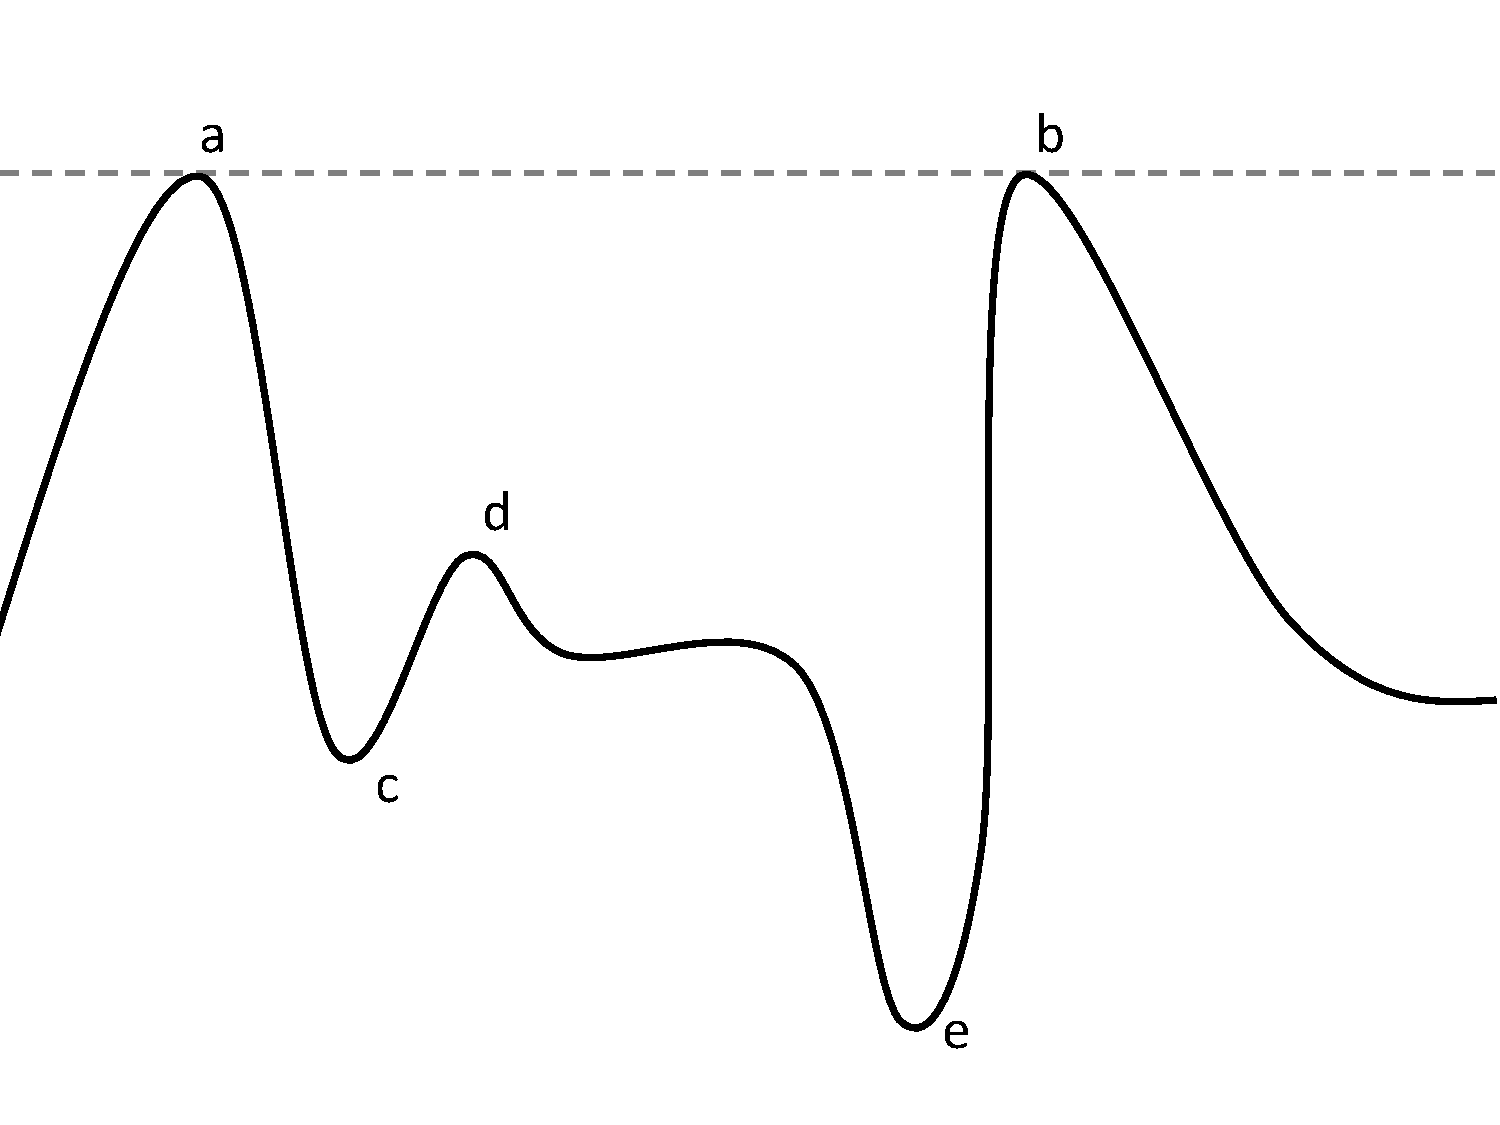
\includegraphics[width=0.4\paperwidth]{searchSpace}
\caption{Examples of local and global optimums.}
\label{localAndGlobalOptims}
\end{figure}

In figure \ref{localAndGlobalOptims}, we can see different examples of global and local optimums. The points labeled \emph{a} and \emph{b} are both global maximums, as they have the same value. The points
\emph{c} and \emph{d} are respectively local minimum and maximum, while \emph{e} is the global minimum.

From all the preceding, we can provide the minimal formulation of an optimization problem as follow 

\definition{Optimization problem}{
\begin{align*}
\text{minimize } &f(x) \\
\text{subject to } &(x \in S)
\end{align*}
Where \emph{S} is the problem search space and \emph{f(x)} the objective function.}

\section{Numerical versus Combinatorial Optimization}

\section{No Free Lunch Theorem}

The No Free Lunch (NFL) Theorems for optimization is a very important result of the field, formalized by Wolpert and Macready \cite{585893}. The basic idea behind these theorems is that no optimization method outperform the others when regarding the class of all the possible problems or, as the authors themselves say,
\begin{quote}
"any two algorithms are equivalent when their performance is averaged across all possible problems." [[give ref on coevolutionnary free lunches]]
\end{quote}
If an algorithm outperforms another on certain types of optimization problems, there must be others classes of problems where this algorithm performs worse.

The NFL theorems are based on several assumptions:
\begin{itemize}

\item the search space is finite

\item the optimization algorithms never re-evaluate the same point

\end{itemize}

The first assumption limit the scope of NFL theorems to the realm of combinatorial optimization, as continuous optimization problems contain by nature an infinity of elements. Indeed, it has been shown that, in the context of continuous optimization, free lunches were indeed possible \cite{Auger-s00453-008-9244-5} (but possibly at the cost of very big memory footprint). Thus this result does not impact directly the scope of this work, but we believe that it is still a good illustration of one of the main problematics of the optimization research field, which is that one must often compromise between [[généralité]] and efficiency. Even in the context of continuous optimization, where the existence of free lunches has been demonstrated, it is probable that we will never find a be-all and end-all optimization technique. This point is for example discussed in \cite{Doe05}.

One example which can be connected to the NFL is the compromise between exploration and exploitation. Basically, an optimization method must often make a compromise between using the previous results to converge toward a region of the search space and exploring the remaining of the search space to find a better region.
For example: some gradient-based methods will use the evaluated points to converge toward a local optimum, but can miss a better solution as they insufficiently explored the search space. On the opposite, some others methods can make a throughout exploration of the search space (by partitioning or random drawing points), but will be slow to converge towards the exact optimum.
It is often possible to parametrize the method to tune the compromise between exploration and exploitation regarding the nature of the problem at hand but, once more, a relevant parametrization requires a sufficient knowledge of the properties of the problem.

Of course, the NFL theorems consider \emph{all the possible objective-functions}. One could argue that "interesting" problems (at least from en engineering point of view) are not distributed evenly over such a space, but correspond to a subset for which some optimization methods are more efficient than others. This is why optimization as a scientific research domain make sense. 

This distinction has been formalized by differentiating \emph{incompressible} from \emph{compressible} objective-functions. Incompressible objective-functions are random and it is thus impossible to develop an optimization method to find the solution efficiently, since good and bad values are randomly distributed. Of course, such "impossible" objectives function make for the major part of all the possible objective-functions \cite{English:3-540-45356-3_7}.
As we said, the set of "interesting" objective-functions, or even the set of real-world related ones is much much more restrained. And for this specific category, some optimizers are better than others. 
However, as we will see in the next sections, the variety of "interesting" optimization problems is still important enough to have resulted in a great variety of specific optimization techniques.

One consequence of the NFL is that selecting an efficient optimization method for a given problem requires to have at least a minimum insight on the properties of the problem. No algorithm can be deemed most efficient for the general case.

On a side note, it can be added that, in addition of the case of continuous optimization, the possible existence of free lunches has been demonstrated for coevolutionary \cite{1545946} as well as multiobjective optimization \cite{1299403}.

\chapter{Numerical Optimization}

As we have seen at the end of the last chapter, optimization methods have to make various compromises regarding applicability versus efficiency.  A great variety of methods exits in the literature, from generic methods applicable to a great variety of optimization problems to very specialized methods designed to be efficient in a specific context. These methods can be segregated by the type of problems they aim to solve or some inherent properties of the method.

Some possible criteria to discriminate based on the type of problem:
\begin{itemize}
\item can we obtain derivatives of the functions defined?
\item is the problem linear (or possibly quadratic)?
\item is the problem convex?
\end{itemize}

For the method in itself:
\begin{itemize}
\item is the method able to take in account constraints on the problem?
\item does the method provides a global solution or a local one?
\item is the method deterministic or stochastic?
\end{itemize}

Based on the shape of the search space and our requirements regarding the method, we will try to choose the most adequate optimization method. As always, the more information known regarding the problem, the more we would be able to select a specialized method with a great efficiency. If very few information is known, it could be necessary to use black-box optimization methods, that is methods which do not make assumption regarding the nature of the problem. These techniques can suffice in themselves to get a good-enough result, or can be used as a prelude of more specialized techniques if enough information is gathered.

A rough proposal of organization of the different types of numerical optimization can bee seen in \ref{numerical_optim_tree}.

\begin{figure}
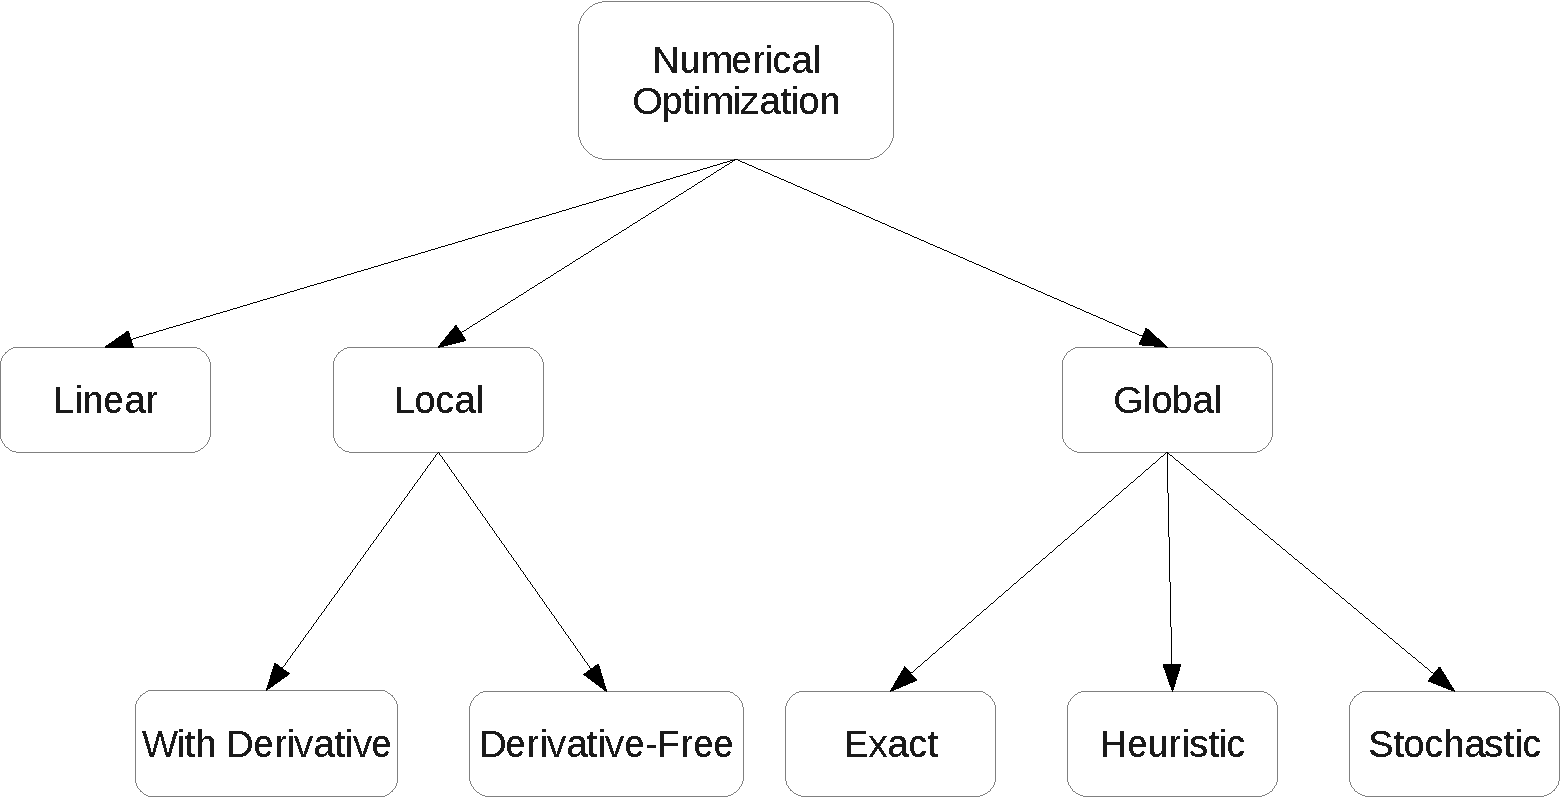
\includegraphics[width=\textwidth]{numerical_optim-crop}
\caption{Types of numerical optimization methods}
\label{numerical_optim_tree}
\end{figure}

Presenting all the numerical optimization techniques would be far outside the scope of this work. In this part we will focus on presenting briefly the different optimization categories we identified on figure \ref{numerical_optim_tree}. We will reference some of the most representatives techniques to illustrate his presentation, but without going into the details of the the techniques. To get a more throughout view of the different techniques, the reader can see reference works such as [[REFS]].

\section{Linear Optimization}\label{linear_optim}

Linear optimization focus on the solving of problems where the objective-function and constraints are linear (that is, $f(x+y) = f(x)+f(y)$ and $f(ax) = af(x)$) and the search space convex.

[[Show what do we mean by convex search space]]

A linear problem with $n$ variables and $m$ constraints can be expressed as:
\begin{align*}
\text{min } & c_1x_1 + c_2x_2... + c_nx_n\\
\text{subject to } &x_i \geq 0, \forall i \in 0,n\\
&a_{11}x_1 + a_{12}x_2 + ... + a_{1n}x_n + b_1 \geq 0\\
&...\\
&a_{m1}x_1 + a_{m2}x_2 + ... + a_{mn}x_n + b_m \geq 0
\end{align*}

This kind of problems is the most basic one. The most well-known method to solve linear problems is the Simplex algorithm\cite{dantzig2003linear}, published by Dantzig in 1947 (based on the work of Leonid Kantorovich). The Simplex algorithm is considered to be the first formal algorithm to solve a numerical optimization problem and to be one of the founding works to the field.

The basic idea of the simplex algorithm is to that the solution space is the convex polyhedron, and the optimal solution is necessarily on one of its vertices. Another property is that a vertex which is not the optimal solution will have at least an edge leading toward a better vertex.
The simplex algorithm starts on one of the vertices, and tries to follow an edge to a vertex which improves the objective-function. The algorithm iterates until it has found a vertex with no edge leading toward a better point (the optimal solution) or until it reaches an unbound edge (in this case the problem is not bounded).

While the simplex algorithm is considered to be very efficient for most cases, some alternatives has been proposed. The most noteworthy is the interior point method and its derivative. Contrary to the simplex method, this methods actually traverses the interior of the solution space (hence its name). The original method proposed by Karmarkar\cite{Karmarkar:1984:NPA:800057.808695} travels through the search space by iteratively finding the best solution over a restricted region delimited by a sphere around the current point.

\section{Local Methods}

Unconstrained local optimization methods concentrate on finding local optimums either because the search space is too big or to complex to find a global optimum in a reasonable time, or because we prefer to quickly find a good enough solution to spend more time to find the best one.
 Moreover, if the objective-function is convex, the local optimum is also the global optimum, in this context local methods can be an easy mean to obtain the best solution.

\subsection{Using Derivatives}

If the derivatives are available, it is possible to propose very efficient optimization techniques to converge toward a local optimum.

In some case, even if the derivatives are not available, it is possible to obtain an approximation of the derivatives using for example a finite difference method. The basic idea of finite difference is to estimate the derivative from the ratio between the variation of the input and the variation of the output of the function.
Basically, if we make the following assumption:

\begin{equation*}f(x + d) \approx f(x) +df'(x)\end{equation*}

then we can estimate the derivative as follow:

\begin{equation*}f'(x) \approx \frac{f(x + d)  - f(x)}{d}\end{equation*}

\subsubsection{Without Constraint}

Methods of this kind can be mostly classified in to broad families: line search and Trust region.
Both families are iterative approaches but differ in the information they use to select the next search point.

The general idea is, from a random starting point $x_0$, to iteratively evaluate a new point using a direction and a step size.
By adjusting the ways the direction and step size are chosen, we can obtain a whole selection of algorithms with varied behaviors.

Formally, from the point $x_i$, the new point $x_{i+1}$ is calculated with:

\[ x_{i+1} = x_i +s_id_i \]

where $d_i$ is the direction vector and $s_i$ the step size coefficient.

\paragraph{Line search}

Linear search is the most basic approach. It first determine  which direction would improve the objective function, then decide of a step size to move toward it.
Some of the most well-known linear search methods are gradient descent, Newton's and Quasi-Newton methods. The gradient method simply uses a step size proportional to the value of the gradient. The Newton's and Quasi-Newton methods however try to find a solution to the equation $\nabla f(x)=0$. The Newton's method use the gradient  and the Hessian matrix of $f$ to estimate a good step size, while the Quasi-Newton method avoid the disadvantages of using the Hessian (which can involve costly operations) by replacing it with an approximation based on the variation of the gradient.

\paragraph{Trust region}

Trust region methods use the neighborhood of the current point to approximate the shape of the objective-function in the neighborhood of the current point. This approximation is the used to find the minimum in a localized region around the current point. These methods are the dual of Line search ones as they start by selecting a step size (the size of the region around the current point) and only after choose the direction.
For example, the Levenberg-Marquardt algorithm, which primary application is least squares problems, uses the Jacobian matrix conjugated with a damping factor to iteratively refine the approximate functions.

\subsubsection{With Constraints}

One of the first proposal for solving constrained problems with derivative is a generalization of interiors points (presented in \ref{linear_optim}). The idea is that a linear function with a non-convex search space can be transformed into a linear function over a convex search space (which is a requirement for applying interiors points techniques), using \emph{self-concordant barrier functions}.
[[BARRIER FUNCTION - WE WILL TALK ABOUT THIS LATER -> MENTION IT ?]]
[[PICTURE OF BARRIER FUNCTION ??]]

A barrier function is a function whose value increases to infinity when its input approaches a fixed boundary.
The idea is to replace the constraint with a barrier function, which is composed to the objective-function. The barrier function is thus used as a penalty for a point which violate the constraint.

For example, taking the following constrained optimization problem:

\begin{align*}
\text{minimize } &f(x)\\
\text{ subject to } &x > 0
\end{align*}

Suppose we are provided a barrier function $b_c(x)$ those value increase toward infinity as x decreases toward 0 ($\lim_{x \to 0^+}b_c(x) = \infty$). We can now use the new unconstrained optimization problem:

$$\text{minimize } (f_{obj}(x) + b_c(x))$$

Another method, which had for some time dominated this part of the numerical optimization field is Sequential Quadratic Programming (SQP). SQP proposes to replace the problem to solve by a sequence of quadratic problems, usually more easily solvable.
SQP is based on a very powerful result of numerical optimization, the Karush-Kuhn-Tucker (KKT) conditions. The KKT conditions are necessary conditions for a solution $x*$ in a nonlinear optimization problem to be a local optimum. They state that, for $x*$ to be a local optimum to an optimization problem with $i$ inequality constraints $gi$ and $j$ equality constraints $h_j$, there must exist some $\mu_i$ and $\lambda_j$ such as:

$\left\{
 		 \begin{array}{l}
			\nabla f(x*) + \sum \mu_i \nabla g_i(x*) + \sum \lambda_j \nabla h_j(x*) = 0 \\
			g_i(x*) \leq 0 \;\forall i \\
			h_j(x*) = 0 \;\forall j \\
			\mu_i \geq 0 \;\forall i\\
			\mu_ig_i(x*) = 0 \;\forall i
		\end{array}
	\right. $
	
The SQP can be viewed as an equivalent of Newton's method to the KKT conditions of the problem.



\subsection{Derivative-Free}

Sometimes we cannot use derivatives in the optimization process, either because the derivatives are not available or too costly to compute.

A very popular method is the Nelder-Mead algorithm. This algorithm places a simplex\footnote{The concept of simplex is a generalization of the concept of triangle in arbitrary dimension. A triangle is a simplex in 2 dimensions, a tetrahedron a simplex in 3 dimensions.It should be noted that the Simplex algorithm, presented in \ref{linear_optim} does not actually use simplices, during solving.} on the search space and applies to it a sequence of transformations by moving its edges.

[[TODO: Picture of Nelder Mead ]]

At each iteration, a new test point is calculated (for example the symmetric of the worst vertex of the simplex regarding the gravity center of the others points). If this point is better than every vertices, then the simplex is stretched toward it. If this point is worse than the current vertices, then we suppose we are stepping over the valley which contain an optimum. In this case the simplex is contracted to be able to explore the valley. Else, we simply replace the worst vertex by the new point.
The iterations stop when the simplex has reach a specified size.


Several derivative-free algorithms interpolate the objective-function with a simpler one. Starting with several evaluation points of the objective-function, we build a simpler function to which we can apply a known optimization method. Based on the result of the optimization, we can update the interpolation model and reiterate.
[[Talk about possible interpolations methods ?]]

\section{Global Method}

While local optimization methods aim only at finding an optimum into a limited part of the search space, global optimization methods aim to find the globally best solution of the problem. Global optimization methods concentrate on providing strategies to explore the search space.

Depending on the nature of the problem, it may be impossible to guarantee that the best solution will be found by any mean other than a complete exploration of the search space (which is in itself an impossible task in the context of continuous optimization).

For example, suppose the following problem:

Minimize $f(x) =$ \begin{cases}
 		 					0& \text{if } x = 1 \times 10^{-9}\\
 		 					1& \text{otherwise} 
 		 			\end{cases}
 		 			
There is no efficient strategy to find the global optimum to such a problem (unless knowing the equations, a thus the solution, beforehand).

Consequently, obtaining the global optimum of an optimization problem with certainty will be possible or not depending on the properties of the problem.
As with local optimization methods, several kinds of approaches have been proposed to solve problems with different properties.

\subsection{Exact Methods}

These methods aims to provide a guarantee about the optimality of the solution. These methods cannot used for any optimization problem, as they need to use some properties of the problem to prove that the solution is a global optimum.

For example, as we said before, if an optimization problem is convex than a local solution is also a global solution. Consequently for convex problem local optimization methods can be used with the guarantee that the solution found will be the best one.

[[
Branch and Bound

Taboo search
]]

\subsection{Stochastic Methods}

[[
Simulated Annealing

Monte-Carlo
]]

\section{Conclusion on Numerical Optimization}

This overview of numerical optimization illustrate how the different optimization techniques range from very efficient but highly specialized methods to board scope methods with slower and more costly strategies.

[[Two axis: Local <-> Global; Specialized <-> Generic]]

\chapter{Multi-Objective Optimization}

Multi-objective optimization (MOO) departs significantly from previous categories of optimization in the fact that you have to consider multiple objective functions instead of one. A main aspect of MOO is the way to conciliate these objectives, which are usually contradictory.
An example of real-world everyday MOO problem could be choosing the mean of transportation for a travel, trying to find a balance between speed and cost. Airplane is the fastest way of transportation, but is expensive. While car is slower, it is cheaper. Train is slower than plane, more expensive than car, but can preferred as the best compromise. There still, however, are solutions which are strictly worse than others (in our example, renting an helicopter would probably be both more expensive and slower than buying a seat on a commercial airplane).
From this example we can see that, for a MOO problem, there rarely is a clear-cut "best" solution. And more importantly that even some solutions which are not optimum for \emph{any} of the objectives can be deemed satisfying. Only when each objective is completely independent, or when no objective is contradictory to another, then a MOO problem can be handled as a set of separated mono-objective optimization problems.
A solution vector which would be optimum for each objective is sometimes called \emph{utopia point}, or \emph{shadow minimum}, and is used as a reference comparison in some of the MOO techniques we present.

[[FORMULATION OF A MOO PROBLEM]]

MOO problems are quite a radical departure from previous optimization problems type we have seen. Many approaches have been proposed, the majority of which can be separated in to categories: \emph{a priori} and \emph{a posteriori} approaches. A priori approaches aims to discriminate between the objectives \emph{before} the optimization process. This often consist into combining the different objectives into one, before applying a classical optimization method on the new, aggregated objective.
On the opposite, a posteriori methods tries to provide a set of efficient solutions among which the decider will choose.
A priori approaches are considered easier, but not very efficient, whereas a posteriori approaches provides more diversity of solutions as well as more insight about the nature of the problem.
A third category can also be considered: the \emph{interactive} methods. Basically, these methods iterates between decision and search phases. For example, an interactive  method could work by quickly providing intermediate solutions to the decision-maker, which would in return refine the search using them.

We will now see some of the strategies have been proposed to deal with such a type of problem.

\section{A Priori Methods}

\subsection{Objectives Aggregation}

The first approach is to transform the MOO problem back to a mono-objective optimization problem, by aggregating the different objectives into one. This can be expressed as follow : \(f_g = aggr(f_1, f_2, ..., f_n)\), where \(f_1, f_2, ..., f_n\) are the original objectives and \(f_g\) the aggregated one, which will be used with classical mono-objective optimization methods.

Concerning the choice of the aggregation function, different strategies can be used.

Concerning the choice of the aggregation function, the simplest strategy is to use a classical function such as addition, multiplication, mean, max or min of the objectives, and variations of the preceding (exponential sum, ...): these methods present the major drawback of requiring the aggregated values to be comparable.[[ Keeping with our travel example]], is it relevant to simply add duration and cost ?

A slightly more sophisticated way is to use pondered mean: we attribute a coefficient to each objective when adding them :

\[ f(x) =\sum_{i=1}^n w_i f_i(x) \]

Where $w_i$ are the coefficients representing the relative preferences between the objectives.

This method allows to express a preference between different objectives, as well as bringing back on comparable scale different objectives. However, one now has to decide of the coefficients to choose. Also, this method can hide some information concerning the solution, for example an extremely poor result in one of the objectives, compensated by small improvements in all the others.  [[Moreover, this solution present some limitations when the solution space is nonconvex [[EXPAND]]]]

[[To get refs which criticize Weighted sum, see "Survey of multi-objective optimization methods for engineering"]]

\subsection{Lexicographic Method}

In this method, the objectives functions are arranged and optimized by order of importance. The result of the optimization at a given step become a constraint to satisfy for the following steps.

Formally, the problem become an ordered set of optimization problems expressed as follow:

\begin{align*}
\text{min } &f_i(x) \\
\text{subject to } &f_j(x) \leq f_j(x_j^*) \\
j = &1, ..., i-1
\end{align*}

A variation of this method proposes to replace inequalities by equality constraints. [[REF]]

Another variation, sometimes called hierarchical, introduces a constraint relaxation coefficient $\delta$ where the new formulation of the constraints becomes:

\[ f_j(x) \leq \left(1 + \frac{\delta_j}{100}\right) f_j(x_j^*) \]

\subsection{$\epsilon$-constraint Method}

The $\epsilon$-constraint method proposes to change the expression of the problem by keeping only one objective (the one deemed the most important) and transforming the others into inequality constraints.

For example, the problem \[\text{min } f_1, f_2, ...,f_n\] where $f_1$ is deemed the most important objective would be transformed in
\begin{align*}
\text{min } &f_1 \\
\text{subject to } &f_2 \leq \epsilon_2, ..., f_n \leq \epsilon_n
\end{align*}

Where $\epsilon_2, ..., \epsilon_n$ must be chosen by the designer.
Depending of the selection of $\epsilon_2, ..., \epsilon_n$, it is possible to obtain a formulation where no feasible solution exist.
[["Survey of multi-objective optimization methods for engineering" -> Bounded objective function method for some ref about methods to select $\epsilon$]]

\subsection{Goal Programming}

[[REF in "Survey of multi-objective optimization methods for engineering"]]

The idea of Goal Programming (also called Target Vector Optimization) is to fix for each objective an associated goal to reach. Each objective can be over- or underachieving its goal, allowing the designer to provide a rough idea of the initial design goals.

The new objective is to minimize the total deviation $\sum_{i=1}^n |f_i - g_i|$ where $g_i$ is the goal associated to objective $f_i$.

Goal Programming is very easy to use and quite popular, and can work even when the designer provided some unreachable goals, but provides no guarantee for the optimality of the solution.

\subsection{Min-Max Method}

This method use the separately attainable minima of the objectives (the so-called \emph{utopia point}) and try to minimize the maximum deviation of the objectives relative to those minima:

\[ \text{min } f = \text{ max } \left( \frac{f_i - f_i^0}{f_i^0} \right) \]

where $f_i^0$ represent the separately attainable minimum of the objective $f_i$.

This method can also be used similarly to Goal Programming, where the separately attainable minima are replaced by goal given by the designer.

A variant of this method, called weighted min-max, or Tchebycheff method, use the following formulation:

\[ \text{min } f = \text{ max } w_i |f_i - f_i^0| \]

where $w_i$ are coefficient provided by the designer.

[[Talk of variants ??]]

\subsection{Analysis of a priori methods}

A priori methods provide a simple and efficient way to tackle the problem of multiple objectives, as they allow to reduce the problem to a mono-objective one.
However, a drawback of these methods is the need for the designer to have a good knowledge of the problem, to know the correct way to combine/compare the different objectives functions. In the general case, the designer could not have enough experience or information to make such decision.

In the case where the designer would have enough knowledge to meaningfully use such a method, the introduction of this knowledge can risk to introduce a bias in the resulting solution, orienting the optimization process toward "standard" solutions at the expense of possible non-conventional ones.

Moreover, aggregations techniques tend to break when the objectives are not comparable, requiring once more knowledge from the designer to introduce adjustment coefficients to re-equilibrate the aggregation function.

\section{A Posteriori Methods}

We have seen that, while convenient, \emph{a priori} methods can be quite restrictive. By choosing beforehand a way to aggregate the objectives, we lose in diversity of solutions and influence the result of the optimization process.

\subsection{Pareto Dominance}

A radically different approach has be proposed, using the concepts of Pareto dominance and Pareto optimality. These concepts were originally been developed in economical sciences first by Francis Edgeworth and later Vilfredo Pareto. The initial application of the concepts was to propose a minimal definition of "efficiency", regarding allocation of resources inside an economical system.

The main idea is that a state where it is impossible to improve the resources allocation for an individual without worsening the situation of at least another is described as \emph{Pareto efficient}, or \emph{Pareto optimal}.

Conversely, if from a system state A it is possible to find a new state B where at least one individual's situation is improved without worsening the situation of another, the state A will be said to be \emph{Pareto inefficient}. The state B will be said to \emph{dominate} the state A in terms of Pareto optimality, and the passage from A to B will said to be a \emph{Pareto improvement}. This relation of Pareto dominance is usually noted \(\prec\).

\definition{Pareto-dominance}{Given A and B two vectors describing different resources allocations in a system, \(A \prec B \Leftrightarrow (\forall i \text{ }A_i \leq B_i \land \exists j \text{ } A_j < B_j\)). }

Note that in the preceding example, we wanted to maximize resources allocation, so \(A \prec B\) reads " B dominates A". If we want to \emph{minimize} the allocation, the meaning is inverted and  \(A \prec B\) reads "A dominates B".
As it is the standard convention in optimization to express problems in terms of minimization, for the rest of this thesis we will use \(A \prec B\) with the meaning of "A dominates B", unless otherwise specified.

Based on this relation of dominance, it is possible to provide a definition of Pareto-optimality.

\definition{Pareto-optimality}{A solution vector that is dominated no other possible solution is said to be Pareto-optimal.}

\definition{Pareto front}{the set of Pareto-optimal solutions.}

It is also possible to classify the solutions by rank: a solution which is dominated by no other is said to be of rank 0 (and to be Pareto-optimal). A solution which is dominated by at most a solution of rank 0 said to be of rank 1 and so on.

As a remark, these definitions of efficiency and optimality do not give any information about the fairness of the allocation, or the well-being of the involved parties. From this point of view, a monopolistic situation where one actor would control all the available resources is as optimal as a situation where all the resources are equally divided between the individuals.

These definitions of dominance and optimality can be used to characterize the possibles solutions of MOO problem. In this case, the problem is no more to find an optimal solution, but to find the Pareto front of the problem.

An illustration of Pareto front can be seen on figure \ref{Front_Pareto}. The elements A and B are Pareto-optimal, while C is not.


\begin{figure}
\centering
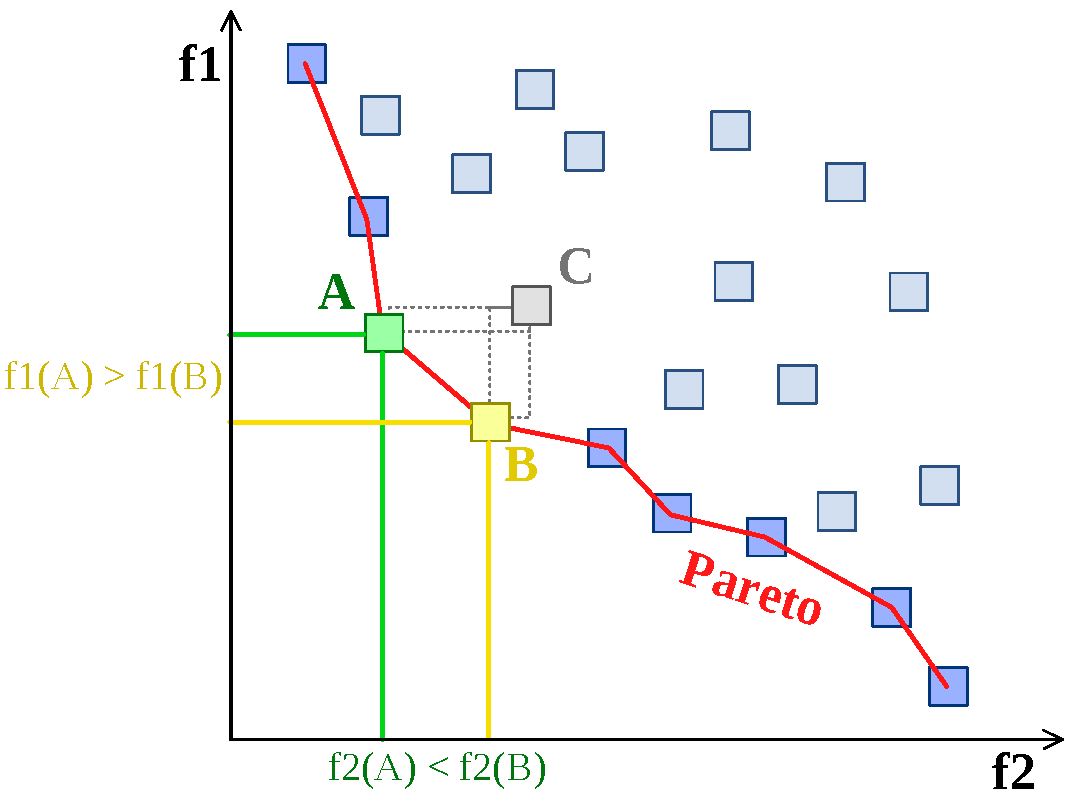
\includegraphics[width=0.4\paperwidth]{Front_pareto}\\
%\hfill\includegraphics[width=6em]{by-sa} \href{http://en.wikipedia.org/wiki/File:Front_pareto.svg}{\begin{small}Johann Dréo\end{small}}
\caption{Illustration of the notion of Pareto Front (CC-BY-SA \href{http://en.wikipedia.org/wiki/File:Front_pareto.svg}{Johann Dréo)}}

\label{Front_Pareto}
\end{figure}

[[TODO: give some example of Pareto methods]]

\subsection{Transforming A Priory Approaches}

A first possibility is to use an a priory method and iterating over it while varying the different parameter to obtain a set of solutions.

[[Example Weighted sum]]

\subsection{Normal Boundary Intersection Method}

Normal Boundary Intersection (NBI)\cite{S1052623496307510} method provides a even distribution of Pareto-optimal solutions using a parameter vector $w$ provided by the designer.

The method use 

[[Explain it]]

One drawback of NBI is that it can produce solutions sets which contain non Pareto optimal-points, as well as overlook some points which are Pareto-optimal.

\subsection{Normal Constraint Method}

Normal Constraint (NC) method tries to improve on NBI by introducing a Pareto filter to avoid the selection of non Pareto-optimal points.

\subsection{Evolutionary Algorithms}

[[Talk about scalability problems -> "Techniques for Highly Multiobjective Optimisation: Some Nondominated Points are Better than Others" by David Corne and Joshua Knowles]]


A widespread strategy to find the Pareto front is to use [[population-based]] metaheuristics, such as Multi-Objective Evolutionary Algorithms (MOEA). 

Historically, evolutionary algorithms are divided in two main categories, based on whether or not they use elitism mechanisms, with some consensus concerning the superiority of elitist algorithms.

\subsubsection{Non-elitist evolutionary algorithms}

[[Vector Evaluated Genetic Algorithm (VEGA) Schaffer (1985) => Non Pareto]

[[  Goldberg and Richardson (1987) =>  Simple Pareto domination scheme. • Sharing on whole population]]


\subsubsection{Elitist evolutionary algorithms}

Different possibilities has been explored to introduce elitism in MOAE. A common approach is to use a second population consisting of elite, non-dominated individuals, which are used as recombination partners for the main population.

[[Signal that evolutionary algorithms have difficulties with more than two objectives ?]]

\section{Interactive Methods [[?]]}

\chapter{Optimization under Uncertainties}

In a pure mathematical world, all models are perfectly correct and have an infinite precision. However, in the physical world, our knowledge can be extremely limited. Moreover, high precision models can require a long time to be computed, making them prohibitively costly when used in the context of an optimization process. At last, when the optimization problem is complex, a small approximation can result in large variations of the output, if the system is sensitive to parameters variations.

[[ILLUSTRATE THE SENSIVITY PROBLEM WITH AN EXAMPLE]]

In order to tackle these issues, several works have been done to take in account uncertainties into the optimization process. We propose to make a quick tour of the different ways which have been propose to model and propagate uncertainties.
A major concern regarding the modeling of uncertainties is the uncertainties \emph{propagation}. 

\section{Several types of uncertainties}

[[TALK ABOUT system vs experimental vs modeling uncertainties ?]]

A distinction is usually made between \emph{aleatory} uncertainties and \emph{epistemic} uncertainties.

Aleatory uncertainties are inherent to the studied system. They can represent for example variability in the material used, a physical variation regarding the manufacturing of some piece, the meteorological conditions to which a device will be exposed etc.
These uncertainties are \emph{irreducible} as it is impossible to remove them with a better analysis of the system.

Epistemic uncertainties result from an incomplete knowledge regarding the system. These uncertainties can result from a limited set of data or lack of knowledge regarding a physical phenomenon.
The uncertainties are \emph{reducible} as it is possible to remove them with a better analysis of the system. However, removing epistemic uncertainty can often be too costly or too difficult in practice, thus still need to be taken in account during the optimization process.

For example, let's suppose we work on a model taking two variables as input and producing an output: $z=f(x,y)$.
Based on known uncertainties on the inputs and the model, how easy it is to combine and propagate these information to determine the uncertainty regarding the output ? Or more formally, can we provide a propagator $P$ such as $u_z = P(u_x, u_y, u_f)$ (where $u_i$ is the uncertainty associated with the element $i$)? As we will see, the ease to obtain such a propagator $P$ depends on the chosen way to model the uncertainties.

\section{Uncertainties Modeling Techniques}

\subsection{Probability Theory}

[[Dans la mise en oeuvre, dire qu'on a utilisé celle là comme exemple parce que c'est la plus commune, qu'elle est bien comprise, et qu'il est facile de trouver des outils pour la manipuler]]

Using the probability theory, uncertainty can be modeled using a distribution function. This modeling provides the advantages of a well-studied theoretical foundation, providing well-known combination and propagation techniques.

Aleatory uncertainties can be characterized by obtaining a distribution function from a data sample.
Well-known statistical techniques can be used to see for example if a data sample follows a known probability distribution, measuring \emph{goodness of fit}, that is, how well a data sample follows a given model, such as the Kolmogorov-Smirnov test \cite{Massey_1951}. 
However, care must be taken as these techniques can introduce some more epistemic uncertainties which can lead to misleading results (for example in the case of insufficient data samples).

Concerning epistemic uncertainty, it can be more difficult to estimate a relevant distribution function  [[TO EXPAND]]

\subsection{Interval Analysis}

Interval analysis can be an alternative to probability theory when the lack of information impeded modeling with a probability distribution, but where the uncertainty can still be bounded within a certain domain.
How easy it is to propagate intervals depends on the involved models. For example in the case of a monotonic function the lower and upper bounds can be determined easily. In the general case, determining the boundaries is equivalent to solving an optimization problem and can thus be solved by using optimization algorithms. In the most extreme cases, one can apply sampling techniques, but this can become quite expensive.
For some examples of existing techniques, one can refer to \cite{Kreinovich_2008}.

A limit of interval analysis is the lack of a measure equivalent to probability, which limit the [[interest]] of this representation in the general case. This modeling can still prove useful in the context of worst case studies where inputs variables can be bounded with accuracy.

\subsection{Fuzzy Sets}

[[Add some ref]]

Fuzzy Sets can be seen as a compromise for when we still lack enough information to use probability theory, but we have more knowledge than just the bounds of the uncertainty.

Basically, fuzzy sets are sets where the membership of an element to the set is not absolute but gradual.
In classical set theory, an element is or is not a member of a set. This notion can be formalized as a function $f_S: X \rightarrow \{0,1\}$ where 
$\left\{
 		 \begin{array}{rcr}
			f_S(x) = 0 \Leftrightarrow x \not\in S\\
			f_S(x) = 1 \Leftrightarrow x \in S
		\end{array}
	\right. $

In the context of fuzzy sets, the equivalent function could be formalized as $f_S: X \rightarrow [0, 1]$, where $f_S(x)$ represents the degree of membership of $x$ to $S$. A value of 1 indicates a total membership to S, a value of 0 a complete absence of membership to S and the values in between specific degrees of membership.
In this regard, fuzzy sets can be seen as a generalization of classical sets.

Fuzzy Sets quantification capability to represent vague information make it attractive to model epistemic uncertainty, as it is more precise than interval analysis and well-suited to express expert knowledge. However this modeling is less powerful and expressive than probability theory, lacking for example a mean to represent an uncertainty measure equivalent to the probability of the probability theory. Indeed, the membership function is insufficient to characterize the likelihood of non-connected events.
To overcome this limitation, the fuzzy set theory was extended into the possibility theory.

\subsection{Possibility Theory}

[[Add some ref]]

Possibility theory seems similar to probability theory. However, they are based on axioms which diverge on a fundamental point.
The probability theory is based on the axiom of \emph{additivity}, which says that for two disjoints sets $U$ and $V$, $P(U \cup V) = P(U)+ P(V)$, that is the probability of at least one of two mutually exclusive events to be verified is the sum of the probabilities of each event.

The possibility theory contains instead an axiom of \emph{sub-additivity} saying that for two disjoints sets $U$ and $V$, $\Pi(U \cup V) = \text{max }(\Pi(U), \Pi(V))$ (where $\Pi(X)$ reads as "possibility of X").

Let's take the basic example of a door which can be either open or closed. If we assume "the door is closed" has a probability of 1, it must follow that "the door is open" has a probability of 0, since the sum of these two complementary events must be 1.

In the context of possibility theory, if we state that the possibility of "the door is closed" is 1, it is not incompatible with the possibility of the door to be open to be, for example, 0.4.

The intuition behind this difference is that probability theory applies to the reality, while possibility theory applies to the knowledge one has regarding the reality, taking in account the "fuzziness" of one's knowledge. To cite the definition proposed by Nikolaidis et al. \cite{nikolaidis:386}:
\begin{quote}
"Possibility measures the degree to which: a) A person considers that an event can
occur, or b) The degree to which the available evidence does not contradict the
hypothesis that the event can occur."
\end{quote}

As well as the notion of \emph{possibility}, possibility theory introduces the notion of \emph{necessity}. Basically, $Nec(U) = 1 - \Pi(\bar{U})$.
This definition implies several interesting properties:

$\left\{
\begin{array}{l}
Nec(U) \leq \Pi(U)\\
Nec(U) + \Pi(\bar{U}) = 1\\
\text{either } \Pi(U) = 1 \text{ or } Nec(U) = 0\\
\end{array}
\right.$

Necessity and possibility of an event $e$ can be viewed a lower and upper bounds to the probability of $e$.

Possibility theory offers numerous tools similar to the ones of probability theory (so much that it was debated if the two theories are really different or if possibility theory was just a variation on probability theory). However, the capability of this theory to model expert knowledge specifically has made it quite popular in the context of uncertainty modeling.

\subsection{Evidence Theory}

[[Add some ref]]

Evidence theory, also known as Dempster-Shafer theory (DST), takes in account available evidences to provide a degree of belief concerning a fact.
The basic idea of this theory is to represent the notion that, the more evidences seems to confirm a proposition, the more we can belive the proposition is true.

Evidence theory represents a proposition as a set of elements. Thus some propositions can includes others propositions (following the basic set inclusion definition). To these sets are assigned a basic belief assignment (BBA), also called \emph{mass}.

From this mass can be calculated two measures:

\begin{itemize}
\item \emph{Belief:} $bel(S) = \sum_{S'\subseteq{S}} mass(S')$
\item \emph{Plausibility:} $pl(S) = \sum_{S'|S' \cap S \neq \emptyset} mass(S')$
\end{itemize}

The mass measurement represents the amount of evidences which support the proposition, the likelihood of $S$. The belief and plausibility can be seen as lower and upper bounds to this likelihood.

Once again we can obtain some interesting properties regarding these measures:

$\left\{
\begin{array}{l}
bel(S) \leq mass(S) \leq pl(S)\\
pl(S) = 1 - bel(\bar{S})\\
bl(S) + bl(\bar{s}) \leq 1\\
pl(S) + pl(\bar{s}) \geq 1\\
\end{array}
\right.$

As with possibility theory, belief and plausibility can be used as lower and upper bounds for probability.

Several rules have been proposed to combine informations coming from different (potentially conflicting) sources. To see an overview of these proposals, the reader can refer to \cite{sentz2002combination}.

\section{Using Uncertainty for Robust Optimization}

[[GIVE EXAMPLE OF SEQUENTIAL OPTIMIZATION (AS DONE WITH ICA), FOR A SIMPLE OPTIM UNDER UNCERTAINTY TECHNIQUE]]

\subsection{Taguchi Method - The firsts steps of Robust Optimization }

Robust optimization tries to provide a solution which is both good and insensible to small variations of the inputs.

The research on robust optimization has been initiated with Taguchi's robust design methodology[[REF]], aiming at improving the quality of manufactured goods.
In his methodology, Taguchi proposes a three-stages process :
\begin{itemize}
\item System design, where the designers determine the overall structure of the product at a high conceptual level;
\item Parameter design, where the optimal values of the design variables are determined;
\item Tolerance design, which focus on reducing the variability of the  various parameters to fix an acceptable limit to the variability of quality for the product.
\end{itemize}

To help the designers during the parameter design phase, Taguchi introduced several measures, among them the Signal-to-Noise (SN) ratios. These ratios are used to estimate the sensitivity of a performance of the product to variations. Each ratio relate to a possible goal regarding the studied performance: larger the better, smaller the better, on target the best. These ratios are respectively noted $SN_L$, $SN_S$ and $SN_T$.
By simulation or experimentation, one must first produce a data set.

The $SN_L$ and $SN_S$ can be directly calculated as

\[SN_L = -10\text{log}\left( \frac{1}{n} \sum_{i=1}^n \frac{1}{y_i^2} \right)\]
\[SN_S = -10\text{log}\left( \frac{1}{n} \sum_{i=1}^n y_i^2 \right)\]

For $SN_T$, we need first to measure the mean response, given by $\bar{y} = \frac{1}{n}\sum_{i=1}^n y_i$
This mean can then be used to calculate the standard deviation as follows 
\[S = \sqrt{\sum_{i=1}^n \frac{(y_i - \bar{y})^2}{n-1}}\]
[[REALLY GIVE THE FORMULAS OF MEAN AND STD ??]]

 $SN_T$ can then be calculated as
 
 \[ SN_T = 10\text{log}\left(\frac{\bar{y}^2}{S^2}\right) \]
 
To reduce the sensitivity of the solution to noise, the SN ratio must be maximized. To this end, Taguchi use the Design of Experiment, a statistical procedure for determining the effect of multiple inputs on a desired output. [[GIVE A REF ON DOE]]

[[EXPAND ON DOE  ?]]

\subsection{}

\chapter{Optimization in Dynamic Environments}
A special case of optimization is optimization in dynamic environment. In these kind of problems, the objective-function is likely to change with time.
Classical optimization techniques fail to solve this problem as they are not meant to take in account the dynamic of the problem.
These problems require specific optimization techniques able to both find a moving optimum and to follow it when it changes.

\section{Genetic Algorithms}

\chapter{Multidisciplinary Optimization}

Multidisciplinary Design Optimization, often abbreviated Multidisciplinary Optimization (MDO), concerns the optimization of complex systems which involves several interacting disciplines. Each discipline in itself can contain this own variables, objectives and constraints. These problems often involves several of the optimization problematics we examined in the previous [[chapters]] (non-linearity, multiples objectives and constraints, uncertainties etc.) and are usually too complex to be handled by classical optimization methods, as evaluating the global function of the problem would be considered too costly.
These kind of problems are commonplace in the industry, especially in aeronautic and aerospace engineering, where parts of the design are often done by different experts teams. For example [[the designing of]] an aircraft can be formalized as a MDO problem involving several disciplines such as mechanic, aerodynamic, acoustic etc. (see \figurename\ \ref{aero-disc}).

\begin{figure}
\centering
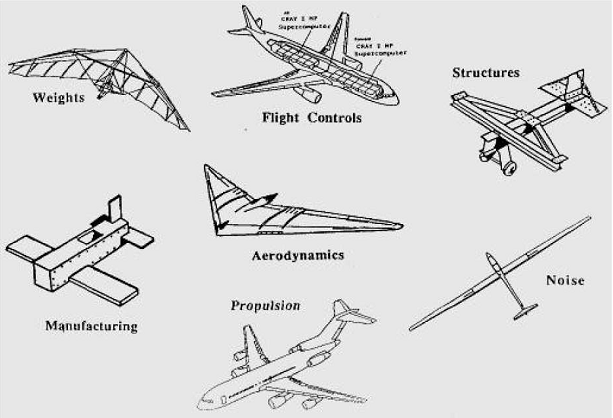
\includegraphics[width=0.4\paperwidth]{Disciplines_Avion}
\caption{Examples of aeronautics disciplines}
\label{aero-disc}
\end{figure}

To handle such complex system, most strategies propose to decompose it into several sub-system of lesser complexity. Concerning engineering, several decomposition strategies have been proposed [[REF Decomposition and Representation Methods in Mechanical Design]]:

\begin{itemize}
\item product (also called object) decomposition, based on the physical components of the system. This kind of decomposition is not always adequate and often subjective;
\item process  (also called sequential) decomposition, based on the work-flow of elements/informations involved into the design process. This decomposition is most adequate when the design process is linear.
\item domain (also called aspect) decomposition, based on the knowledge domains, the disciplines, involved. This kind of decomposition is the basis of MDO methods.
\end{itemize}

[[The AIAA MDO Technical Committee proposed the following definition of MDO\footnote{\url{https://info.aiaa.org/tac/adsg/MDOTC/Web\%20Pages/aboutmdo.aspx}} [[\cite{american1991current}?]]:
 \begin{quote}
"A methodology for the design of complex engineering systems and subsystems that coherently exploits the synergism of mutually interacting phenomena."
\end{quote}]]
MDO methods are not optimization methods \emph{per se}. Instead they focus on providing a optimization strategy for optimizing the different disciplines while maintaining a global coherence. In fact, the optimization of the disciplines is done using classical optimization methods such as presented above. [[In this regard, MDO methods could be seen as optimization meta-methods, or methodologies, as they provide methods to best apply optimization methods to a complex problem. Martin and Lambe\cite{Lambe:2011:A} note the volumes of different terms which have been used in the literature :  "architecture, "method", "methodology", "problem formulation, "strategy", "procedure" or "algorithm". While these authors choose to use the term "architecture", we will stick in this work to the designation of "method", not as a disregard for their arguments but solely for the sake of  consistency.  ]] 

Alexandrov and Lewis illustrated their discussion on Collaborative Optimization\cite{NataliaM.:2000:ACA:886733} with the following theoretical test case:

[[Notion of Standard form]]

\begin{align*}
a_1 &= A_1(s, l_1, a_2) \\
a_2 &= A_2(s, l_2, a_1) \\
\text{minimize } &f(s, a_1, a_2) \\
\text{subject to } &g1(s, l_1, a_1) \geq 0 \\
								&g2(s, l_2, a_2) \geq 0
\end{align*}

[[Add graphical representation]]

It can be noted that this formulation does not differ from the formulation of standard optimization problem. Indeed, as noted by Martin and Lambe\cite{Lambe:2011:A}:
 \begin{quote}
 "If we ignore the discipline boundaries, an MDO problem is nothing more than a standard constrained nonlinear programming problem: we must find the values of the design variables that maximize or minimize a particular objective function, subject to the constraints."
\end{quote}
[[As we will see later, this point is one of the funding principles of the work presented in this thesis.]]

A very common strategy used by most MDO methods is to reformulate the problem to \emph{decouple} variables which are shared among the disciplines. 
For example, the following optimization problem:

\begin{align*}
\text{Minimize } f(f_1(x), f_2(x))
\end{align*}

(where $f_1$ and $f_2$ represent two disciplines depending on $x$)

could become :

\begin{align*}
\text{Minimize } &f(f_1(x_1), f_2(x_2))\\
\text{s.t. } &x_1=x_2
\end{align*}

The shared variable $x$ has been replaced by two independent variables $x_1$ and $x_2$, and a new constraint $x_1=x_2$ has been added to ensure the consistency of the design.


Several specific terms are in use in the domain of MDO:

\begin{itemize}

\item \emph{Design variable}: a variable of the problem which can be chosen by the designer. The goal of the optimization process is to find good values for the design variables of the problem. A design variable is said to be \emph{local} (or \emph{private}) if it is relevant to only one discipline, or \emph{shared} (or \emph{public}) if it is used by several of them.

\item \emph{Discipline analysis/Analyser/Simulator}: 

\item \emph{Multidisciplinary Analysis (MDA)}: [[Say that the models can need to be evaluated potentially SEVERAL TIMES during one MDA, to find consistent set of variables]]

\item \emph{Optimizer/Solver}: A classical optimization technique, such as the ones we have seen in the previous chapters. These optimizers can be applied to the problem as a whole or to specific parts.

\end{itemize}



The classical approach to categorize MDO methods was to separate mono- and multi-level methods.
Mono-level methods use a single optimizer and a non hierarchical structure, while Multi-level methods use a hierarchical structure and possibly several optimizers.

[[introduce others ways to separate

=> GENERAL MDO FRAMEWORK of Balling and Sobieszczanski-Sobieski

=> recent works "Multidisciplynary Design Optimization: A Survey of Architectures" says : 

"We now introduce a new approach to classifying MDO architectures. Some of the previous classifications were based on which constraints could be controlled by the optimizer [77, 121]. Alexandrov and Lewis [121] used the term “closed” to indicate that a set of constraints cannot be satisfied via explicit action of the optimizer, and “open” to indicate that it can.
[...]
Tosserams et al. [84] expanded on this classification
scheme by discussing whether distributed architectures used open or closed local design constraints in the system subproblem. Closure of the constraints is an important consideration when selecting an architecture, because most robust optimization software will permit the exploration of infeasible regions of the design space. Such exploration can result in faster solution via fewer optimization iterations, but this must be weighed against the increased problem size and the risk of terminating the optimization at an infeasible point."


[[Do it after presenting the methods but say you will before]]
]]

\section{An Illustration of Coupled Systems Problematics: Fixed Point Iteration}

To illustrate the difficulties caused by coupled system, let's introduce the problematic of Fixed Point.

\subsection{The Problematic of Fixed Point}

Initially, the problematic of fixed point is the following:

\begin{quote}"Considering a function $f(x)$, does a $x_{fp}$ for which $f(x_{fp}) = x_{fp}$ ?"\end{quote}

If such $x_{fp}$ exists, then it is called a \emph{fixed point} of $f$

\definition{fixed point}{$x_{fp}$ is a fixed point of $f \Leftrightarrow f(x_{fp}) = x_{fp}$}

Not every function has a fixed point, and some functions can have more than one. For example the function

$$f(x)=x+1$$

has no fixed point (there is no $x$ for which $x = x+1$), while the function

$$f(x) = x^3$$

has three fixed points: -1, 0 and 1 (cf figure \ref{fixed_points_x_3}).

\begin{figure}
\centering
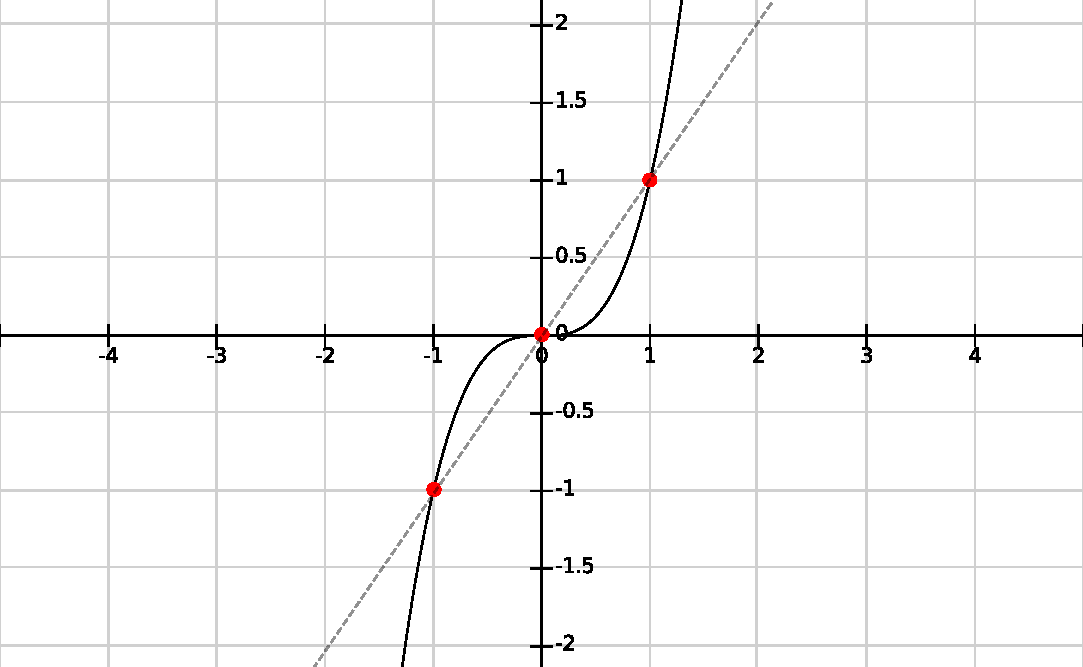
\includegraphics[width=0.4\paperwidth]{fixed_point_x_cube_withdots}
\caption{$f(x)=x^{3}$ and its fixed points, (in dashed grey, the function $y = x$)}
\label{fixed_points_x_3}
\end{figure}

An obvious property of fixed points is that $x_{fp} = f(x_{fp}) = f(f(x_{fp}))$ ...

A fixed point can be \emph{attracting} or \emph{repelling}. A fixed point is said to be attracting when when we converge toward it when iterating over $f$ in its neighborhood. Conversely, a fixed point is repelling if we diverge while doing so. A fixed point which is neither attracting nor repelling is said to be \emph{neutral}.

[[insert diagram of attractive and repelling fixed points]]

A fixed point $x_{fp}$ will be attracting if $|f'(x_{fp}| < 0$.\\
If $|f'(x_{fp}| > 0$ then the fixed point is repelling.\\
At last is $|f'(x_{fp}| = 0$ then $x_{fp}$ is neutral.


\subsection{Fixed Point with Coupled Functions}

The notion of fixed point can be extended to coupled functions.


\section{Mono-Level Methods}

\subsection{Multidisciplinary Feasible}

Multidisciplinary Feasible (MDF), is the most basic and classical MDO method. This approach ensure at each optimization step that the design is consistent as a whole, taking in account all the disciplines together (hence the name). The optimizer only use the design variables, objective functions and constraints.
Basically, MDF alternates between a MDA and a [[global]] optimization phase, ensuring the design to be globally consistent at each optimization step. At each step, the result proposed by the optimizer is used to do a full MDF whose results are used in return for the next optimization iteration.

As it is so straightforward, MDF requires no reformulation of the problem, unlike most of the others MDO methods, and in so is really easy to use. As the design is consistent at each step, the optimization process can provide a solution at any time (but it will not guarantee that the proposed solution will satisfy the constraints, as this concerns depend on the optimization technique used). However, since MDA is supposed to be costly, MDF is often considered to be quite inefficient, since it never exploits the parallelization opportunities dues to the separation of the disciplines. MDF does not provide any guarantee of convergence.

[[formulation + Diagram to illustrate the method]]


\subsubsection{Asymmetric Subspace Optimization}

Asymmetric Subspace Optimization (ASO) is a relatively recent work of Chittick and Martins\cite{Chittick:2007:B} to improve on MDF for MDO problems where some the disciplines are specifically more costly to analyze than the others. The classical illustration given is the one of high-fidelity aerostructural optimization, where the analysis of the aerodynamic is significantly more heavier than the structural analysis. An intermediate optimization phase for the structure is introduced during the MDA, in order to reduce the number of iterations needed at the global level.
This approach can lead to significant improvement over MDF in the context of disciplines with significant analysis costs. However when the analysis costs of the disciplines are comparable, this is approach is less efficient than MDF, as it introduce extraneous optimization step.

It should be noted that this approach is not mono-level as it introduces several optimizers and a hierarchical structure. [[Then why put it here and not in multilevel ?]] 

\subsection{Individual Discipline Feasible}

Individual Discipline Feasible (IDF) differs from MDF in the way that it ensure at each step consistency for each discipline separately, but not consistency between disciplines. The global consistency of the system is not ensured until convergence.
Instead of a full MDA (as in MDF), IDF alternates the optimization with independent disciplines analysis.
However, as the variables shared among the disciplines are not guaranteed to to be consistent, IDF need to introduce a reformulation of the problem where the shared variable are duplicated among the disciplines and several equality constraints need to be added to ensure the eventual consistency.

\subsection{All-at-Once}

All-at-Once (AAO) can be seen a the opposite extreme of MDF, given that it does not try to maintain consistency neither at the global or discipline level during the optimization process until convergence.
All variables are considered as design variable for the optimizer, and the analysis equations are transformed into equality constraints.
This transformation allows the analysis phase to be very quick, as we only need to evaluate the residuals of the equality constraints representing the equations.
However, the drawbacks of IDF are even more important, as AAO requires an even bigger reformulation of the problem, introducing a lot of duplicated variables and consistency  constraints to the problem. This reformulation also complicates the optimization phase.

\section{Multi-Level Methods}

\subsection{Concurrent Subspace Optimization}

Concurrent Subspace Optimization (CSSO) is one of the firsts multi-levels MDO methods. Before the optimization, the problem is decomposed in several subspaces related to the different disciplines. Each optimization iteration then start by a system analysis, followed by a series of subspaces optimization (possibly concurrently), where each optimization tries to solve the global problem by using approximate models of the rest of the system. After the subspaces optimizations, a complete MDA is done to perform a global optimization and update the approximate models.

Originally, CSSO was developed for single-objective optimization problems. However several efforts have been made to extend CSSO to multi-objectives problems.

[[From Concurrent Subspace Optimization for Aircraft System Design -  Ke-shi Zhang:
"In recent years more work (Aute \& Azarm, 2006; Huang \& Bloebaum, 2004; McAllister et al., 2000; McAllister et al., 2004; Orr \& Hajela, 2005; Parashar \& Bloebaum, 2006; Tappeta \& Renaud, 1997; Zhang et al., 2008) has focused on extending existing MDO method to handle such multi-objective MDO problems, by means of integrating a multi-objective optimization method within the MDO framework. This kind of method can be called a multi-objective MDO method.
It is an effective way to integrate multi-objective optimization method within the CSSO framework to develop the multi-objective MDO method. CSSO was extended to solve multi - objective MDO problems, including the Multi-objective Pareto CSSO (MOPCSSO) method, Aeronautics and Astronautics the Multi-objective Range CSSO (MORCSSO) method, the Multi-objective Target CSSO (MOTCSSO) method, the Multi-objective Genetic Algorithm CSSO (MOGACSSO) method and Adaptive Weighted Sum based CSSO (AWSCSSO). In MOPCSSO the Constraint method is integrated within CSSO framework (Huang \& Bloebaum, 2007). In MORCSSO and MOTCSSO the concept of designer preference is introduced (Huang \& Bloebaum, 2004). In MOGACSSO the Genetic Algorithm is combined with CSSO and in the hope of improving the computational efficiency (Parashar \& Bloebaum, 2006). In AWSCSSO the Adaptive Weighted Sum method is introduced into CSSO (Zhang et al., 2008). "]]

\subsection{Collaborative Optimization}

Collaborative Optimization (CO) \cite{Ilan:1994:MOM:887207} reformulate the problem by replacing  dependencies between disciplines by equalities constraints. This transformation allows to solve in parallel discipline-level optimizations problems. A system-level optimizer is then used to minimize the discrepancies (via the added equalities constraints), while maintaining the satisfaction of the disciplines constraints.
CO is best-suited for MDO problems with a low coupling between disciplines. The authors have argued that one advantage of CO is that it closely matches the discipline decomposition of the problem, as the scope domain-specific variables and constraints are limited to the related disciplines. Thus, the discipline optimizations can be done by domain experts  who have a strong understanding of the subproblems.

\subsubsection{ECO}

\subsection{Bilevel Integrated System Synthesis}

Bi-Level Integrated System Synthesis (BLISS) \cite{J.:1998:BIS:886310} has been developed to separate local and shared variables, in order to ease the distribution of the optimization process (be it in regard of expert teams or computational resources).
BLISS shares similarities with CSSO [[explain]]. However, local variables are assigned to the disciplines optimizations while the global variables are assigned to the global system optimization.

For each discipline optimization problem, an approximation of the global objective-functions and constraints is build using linear approximation considering only the variables of the discipline.

The optimization process cycle alternates as follow: First a system-wide analysis is done (which includes the analysis of each subsystem) and used to provide the approximate objective-functions. Then a discipline-level optimization of the objective-functions approximations, which is used for a system optimization concerning the shared variables. These results are then used by the new system analysis at the start of the next step.

\subsubsection{BLISS 2000}
[[DELETE susbusbsection ? => NOPE it is different, see Musltidisciplinary Design Optimization: A survey of Architectures:
"    A radically different formulation called BLISS-2000 was developed by Sobieski et al; . Because BLISS-2000
does not require an MDA to restore the feasibility of the design, we have separated it from the other BLISS variants
in the classification shown in Fig. 7. In fact, like other IDF-derived architectures, BLISS-2000 uses coupling variable
copies to enforce consistency at the optimum. Information exchange between the system and discipline subproblems
occurs through surrogate models of the discipline optima"
]]
   
\subsection{MDO based on Independent Subspaces}

MDO based on Independent Subspaces (MDOIS) \cite{NME:NME1380} has been developed for handling problems where the different disciplines are coupled (i.e. some outputs of one discipline are used as inputs by the others and vice versa) but they do not share any design variable or criterion.
MDOIS decomposes the system in separate subsystems, for each an optimization problem is defined, with its own design variables, objective-function and constraints. The coupling variables are considered constant for these subproblems. After each subsystem has solved its optimization problem, the new values of its variables are used in a system-wide analysis to be re-injected for the next iteration of subsystem optimization.

\subsection{Quasiseparable Subsystems Decomposition}

Quasiseparable Subsystems Decomposition (QSD) \cite{1389-4420} is another specialized method for systems which can be decomposed into subproblems which only depends on local variables and global design variable but not on values produced by others subsystems. 

[[CO/ECO, CSSO, ATC,  BLISS, EPD/IPD, MDOIS, QSD]]

\chapter{Conclusion on Optimization}

We have seen in this part how different types of optimization problems have been defined over time, depending on their topology, their complexity, their specificities.

Something worth noticing is the fact that all these types of problems are not \emph{inherently} different, but share a common structure.
Indeed, a mono-objective optimization problem is just a special case of a multi-objective problem. A multi-disciplinary problem is basically a optimization problem so complex that standard optimization techniques fail.
These distinctions where made because of the limitations of the optimization techniques, which have to choose between being applicable in the general case and being efficient.

An interesting observation concerning MDO techniques is the fact that, to evaluate their performances, they are sometimes applied to simple optimization problems, solvable by numerical optimization techniques (see for example \cite{Kroo:1994:MOM} for an application of CO to the Rosenbrock's valley problem). This observation illustrates the fact that all optimization problems share a common structure and differ only in their complexity. Of course these examples are usually only used as illustration, as MDO methods are too heavy to be interesting to use for such problems.

These conclusions raise an interesting question: could it be possible to create an optimization technique which would scale from simple optimization problems to complex ones?

In itself this statement seems to be contradicted by the intuition provided by the NFL theorems. However we have also seen how at the extreme end of complexity, the concern is not so much about finding an efficient optimization technique, but finding an efficient \emph{organization} to apply specialized optimization techniques to the different parts of the problem, while keeping a global coherence.
At this level, the actual optimization processes can be abstracted as black boxes, which are handled behind the scene by experts or automated processes.

Thus we can reformulate our question as: could it be possible to create a technique which would provide an adequate organization for each type of problem, adapted both to simple problems which need to be solved quickly and to large-scale optimization problem involving whole disciplines?

Currently, only MDO techniques could be seen as being applicable to the whole range of optimization problems, but their strict structure make them to cumbersome for for such a task.
An ideal solution for such a problem would be a method able to adapt itself to the problem at hand, in order to scale with the needs of the engineers.

The next parts of this thesis concentrate on providing such a method.



\chapter{Multi-Agent Systems for Optimization and the AMAS Theory}\label{AMAS_chapter}

As stated in our conclusion on optimization, providing a method able to scale to the needs of the full range of optimization problems will requires it to be capable of adapting to the problem at hand.

The main theme of the SMAC team\footnote{\emph{Systèmes Multi-Agents Coopératifs} (Cooperative Multi-Agent Systems)\\\url{http://irit.fr/-Equipe-SMAC-}}, in which this thesis has been realized, is the Adaptive Multi-Agent Systems (AMAS) Theory. This theory relates to the design of agent-based complex systems with self-adaptive capabilities.

In this chapter we will first describe what multi-agent systems are and how they can be used for problem solving, before concentrating on the concepts of the AMAS theory.

\section{Multi-Agent Systems}

Multi-Agent Systems (MAS) is a relatively recent field which can be seen as the intersection of Artificial Intelligence (AI) and Systems Theory.

%Several specific subfields of AI have been defined, among which we can find automated problem solving, machine learning, robotics, knowledge engineering, planning, affective computing \emph{etc.}. 

As a reminder, the AI field was developed in 1950s as \enquote{the science and engineering of making intelligent machines}, as stated by McCarthy, one of the pioneers of the field \cite{mccarthy2006proposal}. This rather ambitious project was somewhat toned down during the 1970s when the field was the subject of several setbacks leading to an \enquote{AI winter} \cite{10.1109/MIS.2008.20}, whose effects can still be felt today. The commonly accepted reason for this setback was that researchers had been too optimistic in their expectations of the breakthroughs which would be produced by the field, and did not take enough into account the inherent complexity of some of the tasks they were proposing to handle (\emph{e.g.} language processing).

This disgrace period of the AI field ended with the success of expert systems in the 1980s. These systems aim to emulate the ability of a human being to take decisions based on expert knowledge, using inference mechanisms (via an \emph{inference engine}) and a rules database.
However, even expert systems cannot avoid the complexity of modeling knowledge, and are still ultimately limited by the growth of their rules database. This concern, among others (such as privacy of informations) led to a new field of AI named Distributed Artificial Intelligence (DAI) \cite{o1996foundations}, where several expert systems collaborate to provide a collective diagnostic of a situation.

In parallel to the developments of AI, another field of knowledge emerged in the beginning of the century, Cybernetics (also called System Theory), the study of self-regulating systems. Interestingly, this field had radically different origins from AI, taking root in social and natural sciences. These two disciplines had a somewhat uneasy coexistence for some times during the 50s, after which AI took the lead and cybernetics was somewhat relegated in the background (on this topic, see for example \cite{5/2/086.cariani}). The field achieved a revival in the 1970s with the \enquote{new cybernetics}, or \enquote{second-order cybernetics}, which introduces the study of self-organizing systems and the notion of external observer.

It is interesting to note the conflicting nature of AI and cybernetics. AI initially based itself on a reductionist approach of knowledge, using symbol manipulation coming from algebra and logics. Cybernetics was part of the more general epistemological upheaval of Constructivism.

It is at the conjunction of these two seemingly contradictory fields that was born the study of Multi-Agent Systems.

\subsection{Principles of Multi-Agent System}

Before talking about MAS, we must explain the notion of \emph{agent}. Several definitions of what is an agent have been proposed. We keep here the (mostly) consensual one proposed by Wooldridge in \cite{wei1999mutiagent}:

\definition{Agent}{\enquote{An \emph{agent} is a computer system that is \emph{situated} in some \emph{environment}, and that is capable of \emph{autonomous action} in this environment in order to meet its design objectives.}}

Based on this definition, a MAS is a system composed of several agents, interacting among each others and with their environment.

The \emph{autonomy} of an agent is the fundamental characteristic that differentiates it from, for example, the computer science concept of object. While an object is a passive entity encapsulating some data and functions, waiting to be solicited, an agent is capable of acting and reacting with its environment. From this comparison it should be clear that the concept of agent is, like the concept of object, the building brick of a paradigm which can be used to model a complex reality. And indeed, agents have been used in a great variety of fields, a fact which can contribute to explaining the difficulty to produce an unified definition of the concept.

\subsection{Self-* capabilities}

While it is not true for all MAS, some interesting properties can be achieved when taking advantage of the autonomy of the agents. This autonomy, coupled with an adequate behavior of the agents, can lead to systems able to adjust, organize, react to changes \emph{etc.} without the need for an external authority to guide them. These properties are regrouped under the term self-* capabilities (self-\emph{tuning}, self-\emph{organizing}, self-\emph{healing}...).

Not all MAS necessarily present all of these self-* capabilities but, as a result of building a system from autonomous and locally situated agents, many MAS will exhibit them to some degree. Consequently, MAS are often relevant for dynamically taking into account changes in their environment. For example, a MAS in charge of regulating the traffic of packets in a computer network could be able to react efficiently to the disappearance of some of the relay nodes.

\subsection{Multi-Agent Systems for Distributed Problem Solving}

In the context of this thesis, we will concentrate on the application of MAS in the specific context of Distributed Problem Solving (DPS). However it can be useful to bear in mind the others possible application fields: social simulation, biological modeling, systems control, robotics \emph{etc.} and agent-oriented modeling as a programming paradigm in general.

\subsubsection{Multi-Agent Systems for Combinatorial Optimization}

MAS has been applied with great success to multiple combinatorial optimization problems. Many application fields have been proposed, among which \enquote{smart grids} power systems control \cite{RocheLauriBlunierMiraouiKoukam2013_561}, sensors networks \cite{Vinyals3589}, supply chain management \cite{Marik2011, Ka2011.6} \emph{etc.}

A major part of the literature on the application of MAS to combinatorial optimization concerns Distributed Constraint Satisfaction Problems (DCSP, or DisCSP) and its extension, Distributed Constrained Optimization Problems (DCOP, or DisCOP).

DCSP \cite{yokoo1998distributed} is a formalism to model Constraint Satisfactions Problems (CSP) using agents. A CSP is defined as a triplet <$X,D,C$> where:
\begin{compactitem}
\item $X = {x_1, ..., x_n}$ is the set of variables.
\item $D = {D_1, ..., D_n}$ where $D_i$ is the definition domain of $x_i$.
\item $C ={c_1, ..., c_m}$ the set of constraints to satisfy.
\end{compactitem}

The goal is to find an assignment to the set of variables $X$ which:
\begin{compactitem}
\item comply with their definition domains $D$.
\item satisfy the set of constraints $C$.
\end{compactitem}

In order to simplify the representation, the constraints of a CSP are often binary. In this case, the CSP can be represented as a graph where each vertex is a variable and each constraint an edge.

\begin{figure}[]
\centering
	\begin{subfigure}[b]{0.35\textwidth}
			$X = \{x1, x2, x3\}$\\
			$D = \{\{0,1\}, \{1,2\}, \{0,1,2\}\}$\\
			$C = \{(x1 \neq x3), (x2 \neq x3)\}$		
		\caption{formal definition.}
	\end{subfigure}
	\begin{subfigure}[b]{0.45\textwidth}
			\centering
			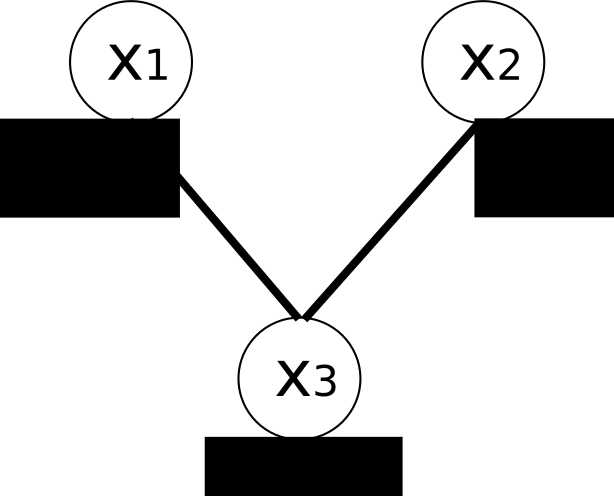
\includegraphics[width=0.7\textwidth]{DCSP}
			\caption{corresponding agent graph.}\label{dcsp:graph}
	\end{subfigure}

\caption{An example of the DCSP representation.}
\label{dcsp}

\end{figure}

From this graph representation, the DCSP formalism models a CSP as an agent graph, with each agent in charge of assigning a value to a variable based on local and shared constraints. A DCSP is described as a quadruplet <$X, D, C, A$>. $X, D$ and $C$ have the same meaning than in the CSP formalism, while $A$ is the set of agents. Each agent in $A$ has the responsibility of a subset of $X$ and knows the constraints related to the variables in its care. The most common assumption is that each agent has the responsibility for one and only one variable. See \figurename{} \ref{dcsp} for an illustration of the graph transformation of a DCSP.

One classical example of DCSP solver is Asynchronous Backtracking (ABT) \cite{Yokoo:2001:DCS:380145}. ABT creates a total ordering on the agents and models the relations between agents as directed links, in order to make the network cycle-free. In ABT agents exchange \emph{nogoods}, which are conditional constraints (the constraint is valid as long as the other agents do not change states). When an agent detects a \emph{nogood}, it checks if it can change its state in order to solve it. If it is possible it does so and informs the agents to which it is linked. Else it propagates it to the lowest priority agent it knows (based on the established ordering) involved in the \emph{nogood}, creating new links if necessary.

An extension of DCSP has been proposed for formalizing Distributed Constraint Optimization Problems (DCOP, or DisCOP). DCOP is to COP the equivalent of DCSP to CSP. While a DCOP is described in the same way than a DCSP, the semantic and goal are different.
In DCOP, the constraints in $C$ represent a decomposition of a global cost function, which the agents try to minimize (or alternatively, maximize). Each constraint is now seen as a local cost function giving the cost associated with each state of the involved variables (in the context of DCOP, the term \emph{constraint} is sometimes replaced by the terms \emph{cost function} or \emph{soft constraint}). Formally, DCOP considers the global objective-function $F(X) = \displaystyle\sum_{x_i, x_j \in X} c_{ij}(x_i,x_j)$ where $c_{ij}$ is a local cost function associated with the states of $x_i$ and $x_j$.

A classical use of DCOP is unsolvable CSP, problems where there is no solution which satisfies all the constraints. In these cases the problem can be changed into a DCOP with the new objective to minimize the number of violated constraints. If we wanted to transform the problem shown in \figurename{} \ref{dcsp} (ignoring the fact that this DCSP is in itself solvable), we could replace the constraints in $C$ by the function $c_{13}$ and $c_{23}$ defined as follows:

\begin{center}
\begin{tabular}{ccc}
\toprule
$\boldsymbol{x_1}$	& $\boldsymbol{x_3}$ & $\boldsymbol{c_{13}(x_1,x_3)}$\\
\midrule
0 & 0	& 1\\
1 & 0	& 0\\
0 & 1	& 0\\
1 & 1	& 1\\
0 & 2	& 0\\
1 & 2	& 0\\
\bottomrule
\end{tabular}
\quad
\begin{tabular}{ccc}
\toprule
$\boldsymbol{x_2}$	& $\boldsymbol{x_3}$ & $\boldsymbol{c_{23}(x_2,x_3)}$\\
\midrule
1 & 0	& 0\\
2 & 0	& 0\\
1 & 1	& 1\\
2 & 1	& 0\\
1 & 2	& 0\\
2 & 2	& 1\\
\bottomrule
\end{tabular}
\end{center}

In the context of this framework, many techniques have been proposed. One of the leading algorithms to date is the Asynchronous Distributed Optimization Algorithm (ADOPT) \cite{Modi06adopt:asynchronous}.In order to work, ADOPT also needs to reformulate the problem by introducing a total ordering on the agents. This ordering allows to create a tree representation of the problem, where each agent has a single parent and multiple children. The algorithm in itself is articulated on two main ideas:

\begin{compactitem}
\item each agent asynchronously changes states when it perceives a possible better solution.
\item the agents can backtrack to previously explored solutions, but only if this current state is worse than a specific \emph{backtrack threshold} determined by its parent agent.
\end{compactitem}

Another well-known algorithm is Optimal Asynchronous Partial Overlay (OptAPO) \cite{Mailler-355}. This algorithm is an adaptation of Asynchronous Partial Overlay (APO), which was proposed for solving DCSP. OptAPO, as APO, is based on the principle of \emph{Cooperative Mediation}, where the agents try to identify parts of the problems which can be solved in a centralized way (using centralized solvers such as Branch-and-Bound). During solving, some of the agents take the role of mediators during \emph{mediator sessions}, where they compute a solution to a part of the whole problem and propose the solution to the others agents involved into the mediation.

The DCOP formalism is very popular in its own right as it allows a clear framework on how to represent this type of combinatorial problems without putting too much restrictions on how the problem is solved. The exact information shared by the agents, and the way they communicate among themselves is not constrained. However this formalism is not without limitations.\\
While some works successfully used DCOP in the context of continuous optimization\cite{stranders2009decentralised}, this formalism is not adequate to handle the full range of continuous optimization problems. DCOP was conceived for a specific type of problems where the difficulty resides in the combination of multiple constraints. These problems are supposed to be easily decomposable into several cost functions, where the cost values associated to the variables states are supposed to be known. This major assumption does not stand for complex continuous optimization problems (such as MDO problems for example), where the complexity of the models and their interdependencies cause this information to be unavailable in most cases. %Modeling such problems with DCOP would be impossible in most case, as most agents would potentially be related to every other agent and the cost functions would be unknown.

It is interesting to note that many methods require non-trivial changes to the topology of the agent graph to work (acyclic graph, tree structure...), both in the context of DCSP and DCOP. These changes can be potentially extensive operations in themselves, and must be done carefully lest the relevance of the results be compromised. In this regard, most existing agent-based optimization techniques for DCOP may require a strong expertise to be efficiently applied\cite{Ka2011.6}.

\subsubsection{Multi-Agent Systems for Continuous Optimization}

While MAS are a popular approach for solving combinatorial optimization problems, their application to continuous optimization is scarce at best. One could explain this discrepancy by the fact that continuous optimization problems are in general more difficult to decompose than combinatorial ones.

As said in the previous section, an adaptation of DCOP with continuous variables has been proposed in \cite{stranders2009decentralised}. This work proposes an adaptation of the max-sum algorithm in the continuous case by redefining the two operations of summation and maximization in order to be able to use them over continuous utility functions. However, this work concentrates on a specific type of problem (distributed sensor networks) and the utility functions must be piecewise linear. It is not applicable to the broader scope of general continuous optimization problems.

Some works have been proposed for using MAS for dynamic continuous optimization (see \cite{lepagnot2010new} for example). However these works usually involve population-based exploration of the search space, where one agent represents a single candidate solution of the problem. These kinds of population-based approaches are ill-suited for complex problems, where a major difficulty is the cost of evaluating a point in itself.

A notable work on the subject of complex continuous optimization is the MASCODE algorithm \cite{welcomme2006self}, which concentrates on MOO and MDO problems. In MASCODE, each agent is in charge of a discipline and the links between agents represent the dependencies between the different disciplines. For each input of a discipline, a \emph{physical validity interval} and an \emph{objective validity interval} are defined. These two intervals represent respectively the physical constraints of the model and the boundaries of an objective to achieve. Using these two measures, a satisfaction indicator is defined using a parametric piecewise continuous function. The basic idea of this satisfaction indicator is as follows: 
\begin{compactitem}
\item when the value of the input is in the boundaries of the objective validity interval, the satisfaction of the agent regarding this input is high,
\item when the value of the input is outside of the objective validity interval but inside the physical validity interval, the satisfaction lowers,
\item if the value of the input goes outside the physical validity interval, the satisfaction becomes minimal.
\end{compactitem}

The agents use the values of their inputs to send \emph{forward messages}, informing others agents of the values of their outputs. Upon reception of these messages, an agent uses these new values to recalculate its own outputs (potentially sending in turn new \emph{forward messages}) and send \emph{backward messages} to the agents controlling their inputs. These \emph{backward messages} are modification requests indicating the satisfaction of the requesting agent. Upon reception of such messages, the agent will select which ones to handle based on the current satisfaction degree of their sender, and will change the value of its inputs accordingly (sending in turn new \emph{backward messages} if required).

This algorithm is very interesting as it makes very few presuppositions concerning the shape of the optimization problem. The problem can be expressed as initially conceived by the designer, without requiring special transformation operations. Still, there are some limitations to the expressiveness of the formulation. The possibilities for the designer to express constraints and objectives of the problem are restricted to the specific use of the physical and objective validity intervals. As a consequence, constraints and objectives cannot be expressed independently, and can only concern \emph{one} variable at a time. While this latter limitation can somewhat be circumvented by introducing artificial disciplines placeholders, the natural modeling of the domain is then lost. This limitation can be explained as a consequence to the specific application domain which was considered for the algorithm (industrial product design).

\subsubsection{Analysis of Multi-Agent Systems for Distributed Problem Solving}

We have seen in this section how MAS have been applied for problem solving. While the solving of discrete constraint satisfaction and optimization problems has been a very popular topic of interest, very few works exist concerning the solving of continuous problems. Among the few existing works, most concentrate on specific application topics, thus no real unified effort exist in this regard comparable to one which can be observed for discrete optimization.

One of the main contributions of this thesis is to rectify to this deficiency by providing not only an agent based method for general continuous optimization but also a general modeling for enabling further contributions on a comparable basis.

\section{The Adaptive Multi-Agent Systems Theory}\label{amas_theory}

\subsection{Theorem of Functional Adequacy}

The design of a MAS for problem solving is not an easy endeavor. We can observe that many of the MAS for problem solving proposed by the scientific community are nature-inspired (ants, flocks, bees, bats etc.) \cite{di2011self}. Indeed, Nature had a long time to experiment on several arduous problem and plenty of subjects at hand. Why would we not take advantage of that? However, such a strategy presents a severe limitation, as it is ultimately restricted into the potential solutions it can provide.
%However, such a strategy presents a severe limitation, as it can bring us existing solutions to apply to potential problems but ultimately cannot help us to find potential solution to some existing problems. By restricting ourselves to nature-inspired mechanisms we are bound to their application field.\\
%The inspiration for things such as the internal combustion engine was not found in nature, since no other biological organism than men ever bothered with something in appearance so foolish as trying to reach for the Moon\footnote{In total honesty, it is possible that some other organisms already tried to reach for the Moon. But it seems such behavior did not give them enough significant evolutionary advantage to be noteworthy (except of course for a specific cow in the popular nursery rhyme \cite[p.~203--204]{opie1997oxford}).}.

In order to overcome this limitation, we need to rely on a more theoretical approach which would help us in the design of MAS for which we do not know any existing applicable mechanisms. Such an approach is provided by the Adaptive Multi-Agent Systems (AMAS) theory.

The AMAS theory was developed by the SMAC team and formalized in \cite{glize2001adaptation}. It focuses on cooperation as the fundamental mechanism of MAS design.

%This modeling is holonic \cite{koestler1989ghost} at its core, since the agents themselves can also be viewed as systems for which the environment consists of the other agents and the environment of the encompassing system.

At the base of the theory is the modeling of a system as a set of entities, the agents, interacting with each others and with their environment. The system can be deemed to be \emph{functionally adequate} by an external observer if this latter judges that the system as a whole correctly accomplishes its function in regard to the environment. This external observer can be considered to be a perfect oracle, in a way similar to the Laplace's demon, knowing exactly which what be the consequences of each interactions between the system and its environment.

It is important to understand that, from a theoretical point of view, the notion of functional adequacy is inherently subjective, and depends on the observer. In practice it is however usually easier to attain a reasonable consensus. For example a natural system will usually be deemed adequate if it survives and thrives in a sustainable way. For an artificial system it is often even easier since the functional adequacy corresponds to the function expected by the designer of the system.

The AMAS theory identifies three categories of interactions between a system and its environment:
\begin{compactitem}
\item Cooperative action: the acting entity is beneficial to the other.
\item Antinomic action: the acting entity is detrimental to the other.
\item Neutral action: the acting entity has no effect on the other.
\end{compactitem}

From this categorization, the theory draws its formal definition (and fundamental axiom) of functional adequacy:

\definition{Axiom of functional adequacy}{A functionally adequate system has no antinomic interaction with its environment}

\begin{figure}
\centering

	\begin{subfigure}[b]{0.45\textwidth}
		\centering
		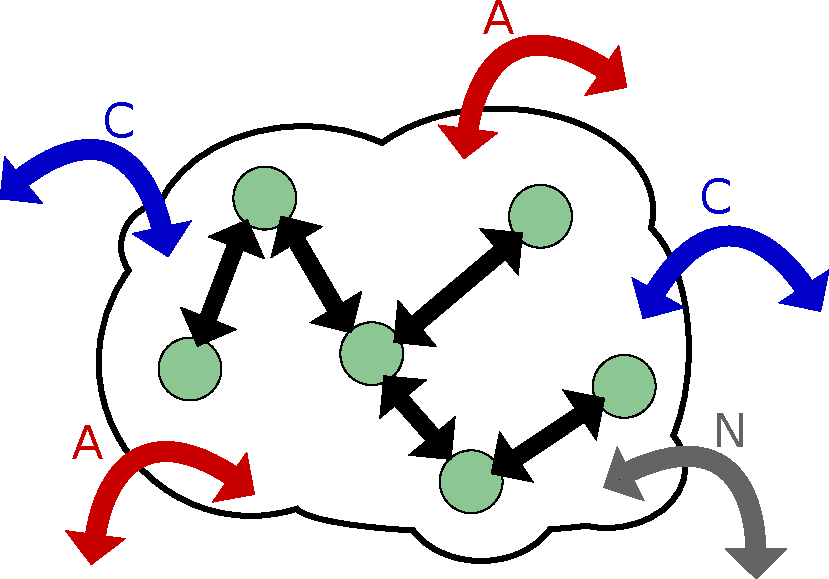
\includegraphics[width=\textwidth]{system_non_adequate}
		\caption{Non functionally adequate system.}\label{adequacy_comp_1}
	\end{subfigure}
	\begin{subfigure}[b]{0.45\textwidth}
		\centering
		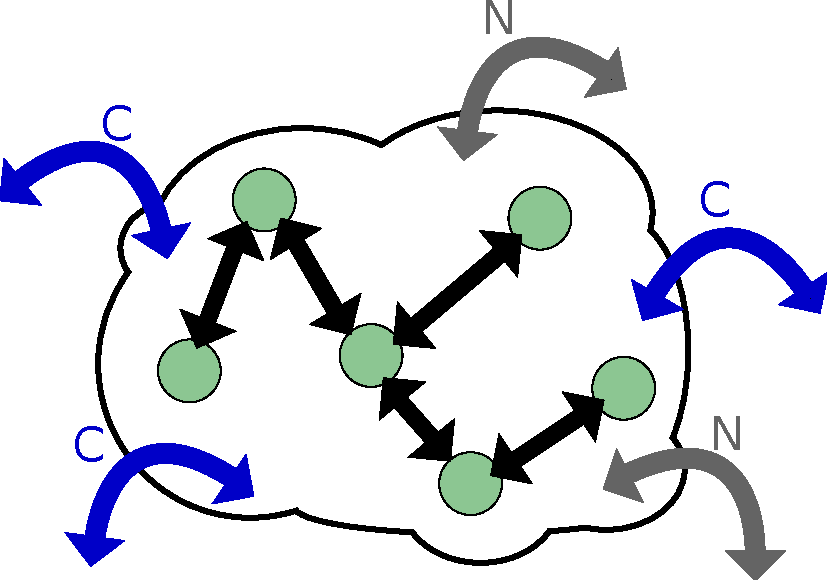
\includegraphics[width=\textwidth]{system_adequate}
		\caption{Functionally adequate system.}\label{adequacy_comp_2}
	\end{subfigure}
	
	\begin{subfigure}[b]{0.45\textwidth}
		\centering
		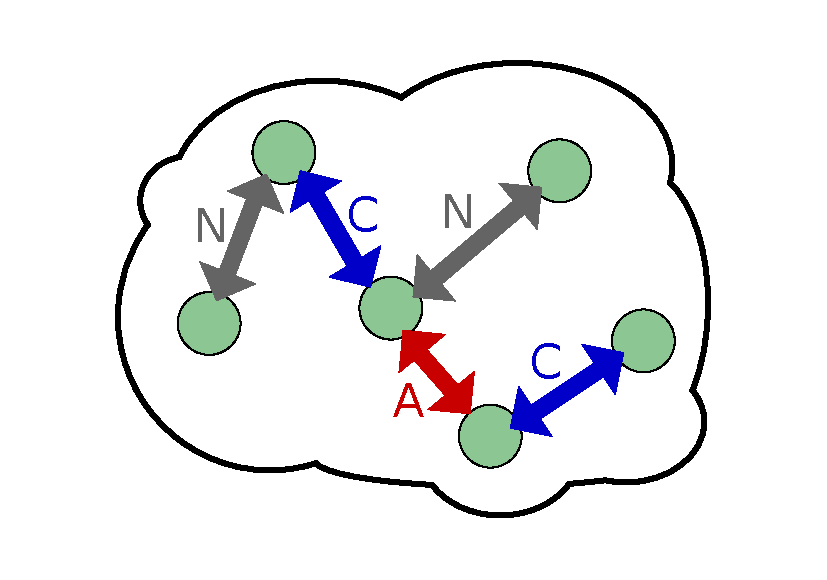
\includegraphics[width=\textwidth]{system_non_cooperative}
		\caption{Non internal cooperative medium system.}\label{internal_cooperative_comp_1}
	\end{subfigure}
	\begin{subfigure}[b]{0.45\textwidth}
		\centering
		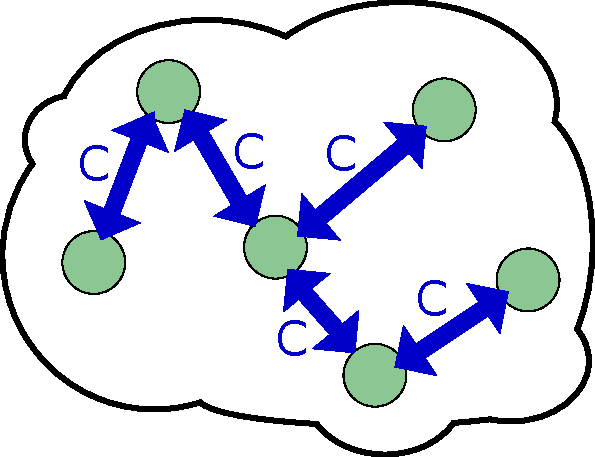
\includegraphics[width=\textwidth]{system_cooperative}
		\caption{Internal cooperative medium system.}\label{internal_cooperative_comp_2}
	\end{subfigure}
	
	\begin{subfigure}[b]{0.7\textwidth}
		\centering
		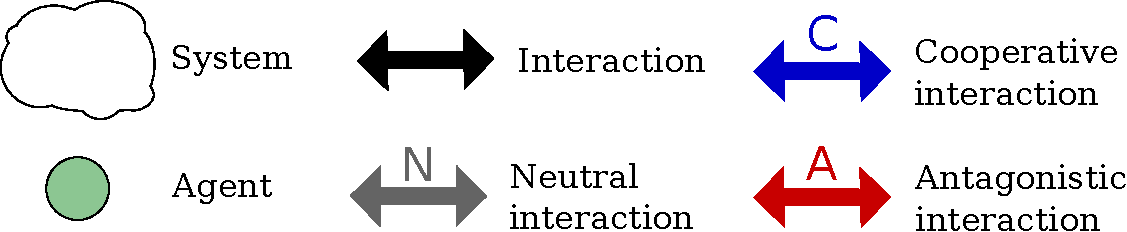
\includegraphics[width=\textwidth]{system_legend}
	\end{subfigure}
	
\caption{Illustration of functionally adequate and internal cooperative medium systems.}
\label{adequacy_comp}
\end{figure}

An illustration this axiom is shown on \figurename{} \ref{adequacy_comp_1} and \figurename{} \ref{adequacy_comp_2}.

%\definition{Internal cooperative medium system}{A system in which the agents only have cooperative interactions with each others or their environment[[?]]}

Using this axiom, several properties have been demonstrated concerning the specific set of \emph{internal cooperative medium systems}, defined as systems in which the agents do not have any antinomic or neutral interaction (illustrated on \figurename{} \ref{internal_cooperative_comp_1} and \figurename{} \ref{internal_cooperative_comp_2}). We will not enter here in the details of these properties and their demonstration, the interested reader can refer to \cite{glize2001adaptation, gleizes1999theory}. Suffice to say that these properties lead to the central theorem of functional adequacy:

\definition{Theorem of Functional Adequacy}{For each functionally adequate system there exists an internal cooperative medium system also functionally adequate in the same environment}

This theorem is at the core of the AMAS approach of system design. We already know that for each problem there is possibly an infinity of equivalent systems producing the same adequate functioning. Using the theorem of functional adequacy we can concentrate on designing an internal cooperative medium system, that is, designing a system were the agents cooperate among themselves and with their environment. The goal of a designer using this approach is thus to study the nature of the interactions between the entities of the problem domain, and to see how the non cooperative situations could be corrected in order to obtain an internal cooperative medium system.

In addition to providing us with a theoretical context, this approach gives us another interesting property: as the design of the system is focused on the local interactions of the agents, we do not need to explicitly take into account the global function of the system. This property is extremely significant. If the global function is complex, it can be extremely difficult to successfully design a system which explicitly tries to achieve the global function (top-down approach). By concentrating on the local functions of the agents, we can spread the complexity and ease the design of the system (bottom-up approach). As such, this approach strongly relies on emergence phenomenons and is often referred to as \enquote{Emergent Problem Solving} \cite{quinqueton2000emergent}.

\subsection{Cooperative Agents and Non Cooperative Situations}

To guide the designer during the building of such internal cooperative medium system, the conditions of what makes an agent a \emph{cooperative agent} have been further formalized. An agent is said to be cooperative if it satisfies three conditions:
\begin{compactitem}
\item $C_{perception}$ Every perceived signal can be understood without ambiguity.
\item $C_{decision}$ Every interpretation must produces useful information.
\item $C_{action}$ Every action done based on the decision must be useful.
\end{compactitem}

Based on these conditions, a set of \emph{Non Cooperative Situations}(NCSs) has been identified. These NCSs correspond to interactions which are not cooperative, and must be removed for the system to be an internal cooperative medium system. The NCSs are classified based on the condition they violate. The table in \figurename{} \ref{NCS} shows this classification.

\begin{figure}
\centering
\begin{tabular}{ll}
\toprule
\textbf{Violated condition}	& \textbf{Corresponding NCS} \\
\midrule
$C_{perception}$ & Incomprehension, Ambiguity\\

$C_{decision}$ & Incompetence, Unproductiveness \\

$C_{action}$ & Uselessness, Competition, Conflict\\
\bottomrule
\end{tabular}
\caption{The conditions for cooperation and corresponding NCS.}
\label{NCS}
\end{figure}

The different NCSs are:
\begin{compactitem}
\item\textbf{Incomprehension} The agent is not able to extract information from a received message.
\item\textbf{Ambiguity} The exact meaning of a message cannot be determined, or lacks required informations.
\item\textbf{Incompetence} The agent does not have the capabilities to handle a received information.
\item\textbf{Unproductiveness} A received information does not lead to any useful conclusion.
\item\textbf{Conflict} The action of the agent is incompatible with an action from its environment.
\item\textbf{Competition} The action of the agent leads to the same result than an action from its environment.
\item\textbf{Uselessness} The action of the agent has no effect on itself or its environment.
\end{compactitem}

A cooperative agent actively tries to avoid these NCSs and, should this fail, to solve them to the best of its capabilities. To this end, three distinct mechanisms can be used\cite{bonjean2009engineering}:

\begin{compactitem}
\item\textbf{1. Tuning} The agent can change one or several of its internal parameters (\textit{e.g.}, adjusting the priorities of its behavior rules).
\item\textbf{2. Reorganization} The agent can change its relationship with its environment (\textit{e.g.}, removing or creating new links with others agents).
\item\textbf{3. Evolution} The agent can change the nature of its environment (\textit{e.g.}, removing or creating new agents).
\end{compactitem}

The order of these mechanisms usually correspond to their level of disruption (\textit{i.e.}, adjusting its parameters usually has less consequences than creating and removing agents). In general, it is preferable to make the less disruptive possible adjustment. One can for example design the agents based on an escalation principle, where the agents try to solve a NCS first by using tuning, escalating to a more disruptive mechanism only when the previous ones failed to solve the NCS. Of course, a NCS situation being by itself disruptive, it is sometime more efficient to immediately make a more radical adjustment in order to solve the NCS more quickly. The designer will have to balance these concerns according to the specificities of the system.

\subsection{The Importance of Locality}

A primordial aspect of the AMAS theory is the importance of locality. The theory insists on the need to consider and consider only the partial knowledge and local interactions between the agents, without trying to provide a \enquote{bigger picture}. While this concern can be linked to specific notions like the concept of emergence, we believe that a direct explanation can be found regarding preoccupations about the \emph{scalability} of the system.

The AMAS theory concerns systems which aim to solve complex problems. By definition the difficulty of such problem increases exponentially with its size. To design a MAS able to scale with the size of the problem, the designer has in general two possibilities: he can increase the size of the system or increase the complexity of the agents. The key difference between these two operations is their marginal costs.\\
While adding a new agent to the system should usually represent a constant cost (in terms of complexity, computational requirements	...), increasing the complexity of the agents will be more and more difficult, since the agents will individually reach the same limitations as centralized methods. The principle of locality is a good example for this argument. Suppose a hierarchical system where one of the agent is in charge of a whole subsystem. If the increase of the complexity of the problems results in an increase of complexity of the subsystem, after some limits the agent will not be able to handle correctly the subsystem, resulting in a limit to the scalability of the system as a whole.

The software engineer will not miss the uncanny similarity of this argument with the relatively recent trend regarding scalability concerns for computer infrastructures (for \emph{e.g.} web servers, distributed databases \emph{etc.}). The two main categories for scaling resources in such systems are \emph{vertical scalability} (scaling \enquote{up}) and \emph{horizontal scalability} (scaling \enquote{out}). Vertical scalability is the improvement of existing resources for them to be able to handle more data/traffic/..., while horizontal scalability consists in adding more resources to spread the workload. While in the past vertical scalability was the dominant practice, the current consensus seems to be that horizontal scalability is easier and provides better performances increase \cite{michael2007scale}.\\
Of course such comparison must be made with caution, as the context of the two fields are quite different. However it is interesting to note how similar concerns from these different fields led to a similar evolution in the approaches.

Obviously, such general principles cannot hold systematically true and some problems which cannot be solved by adding more agents are easily resolved by improving their reasoning capabilities. More so, in some cases increasing the size of the system can increase the complexity of the existing agents (for example by adding neighbors to an agent, thus increasing the complexity of its decision process). Still, in the general case, the motto of approaches such as the one of the AMAS theory could be \enquote{scale out when you can, scale up when you must}. 

\subsection{ADELFE - A Method for Designing AMAS}\label{AMAS-ADELFE}

ADELFE \cite{bernon2003adelfe} is a method dedicated to the development of AMAS. The name \enquote{ADELFE} is the French acronym for \enquote{toolkit to develop software with emergent functionality} (\textit{Atelier pour le DEveloppement de Logiciels à Fonctionnalité Emergente}). While ADELFE is not the only method devoted to guide the design of a MAS, it is the only one specifically tailored for AMAS.

The ambition of ADELFE is to provide be-all and end-all method to guide engineers during all the phases of the design of an AMAS, from the high-level requirements to the \enquote{nuts and bolts} implantation details. This ambition was the driving factor for multiple projects with the objective to improve or complement ADELFE with additional tools, such as the Make Agents Yourself (MAY) framework \cite{No2012.2}, used to automatically generate agent architecture implementations.

However, as for most general engineering methods, a current limitation of ADELFE is that it only provides high-level guidelines concerning the behavior and architecture of the agents, staying at a general, abstract level. This current limitation makes difficult for a non-expert in AMAS to actually provide an adequate instantiation for the problem he wants to solve. It is the same analysis in \cite{Ka2011.6} which led the author to prone a specialized variant of the method containing additional guidelines and tools for applying AMAS in the context of problem solving.

We will go into greater details concerning the inner workings of ADELFE and how this method was involved in the context of this thesis in chapter \ref{ADELFE_chapter}.

\subsection{Conclusion on the Adaptive Multi-Agent Systems Theory}

We presented here the AMAS theory. This theory proposes a way to model systems by their constituting parts, the interactions between themselves as well as with the environment, and identify the special category of internal cooperative medium systems.

An interesting aspect of this theory is that it provides a guidance to build a multi-agent system based on the problem to solve. Classical solving methods often use a very rigid formalism which needs to be followed. For example, genetic algorithms are a very powerful technique, but they require the problem to fit the genetic representation/fitness function model. To use these kinds of methods, one would now be presented with a whole new problem: \enquote{how can I express my problem to fit the solution I want to employ?}

While a non-negligible part of real-world problems are more or less straightforwardly translatable in such formalisms, there is still a whole range of problems for which this translation is not so easy. This can be either because no method adequate enough for the domain was proposed, or because there is no consensual representation of the domain. For these problems, the AMAS theory can provide an interesting asset as the design of the MAS is based on the problem domain. The solution is adapted to the problem, instead of requiring the problem to be adapted to the solution.

We can say that, while the AMAS approach can be applied to any kind of problem, it seems to be especially adequate when trying to solve problems that are still in an exploratory phase, where no \enquote{clear-cut} solution exists.

\part{A Multi-Agent System for Optimization}

\chapter{Agent-Based Modeling of an Optimization Problem}

\section{From an Optimization Problem to a Multi-Agent System}

\chapter{Simulation Rules}

\chapter{Solving Rules}

\chapter{Implementation}

\section{MAY Architecture}

To implement the MAS, we used the Make Agents Yourself (MAY) framework. MAY is a component-based framework which automatically generate an implementation of an agent architecture from a given description.

[[PROVIDE SOME REF -> ASK VICTOR]]

The Adelfe methodology proposes an abstract agent architecture (represented in \fig{[[TODO]]}), which we translated into the MAY architecture description language, SpeADL. [[As our agents only act and communicate using message-passing, we could make some simplification concerning the modeling of the communication and action capabilities.]]
All our agents use the same AMAS architecture. They are differentiated by specific implementations of the components. For example, \emph{Model} and \emph{Variable} agents will have different implementations of the \emph{Behavior} component.

For the sake of clarity, the agent architecture is separated in three views: the \emph{behavior}, \emph{communication} and \emph{monitoring} views.

\subsection{Behavior}

The \emph{behavior} view (\figurename \ref{Arch-behavior}) contains the components related to the behavior of the agent. 

\begin{figure}
\centering
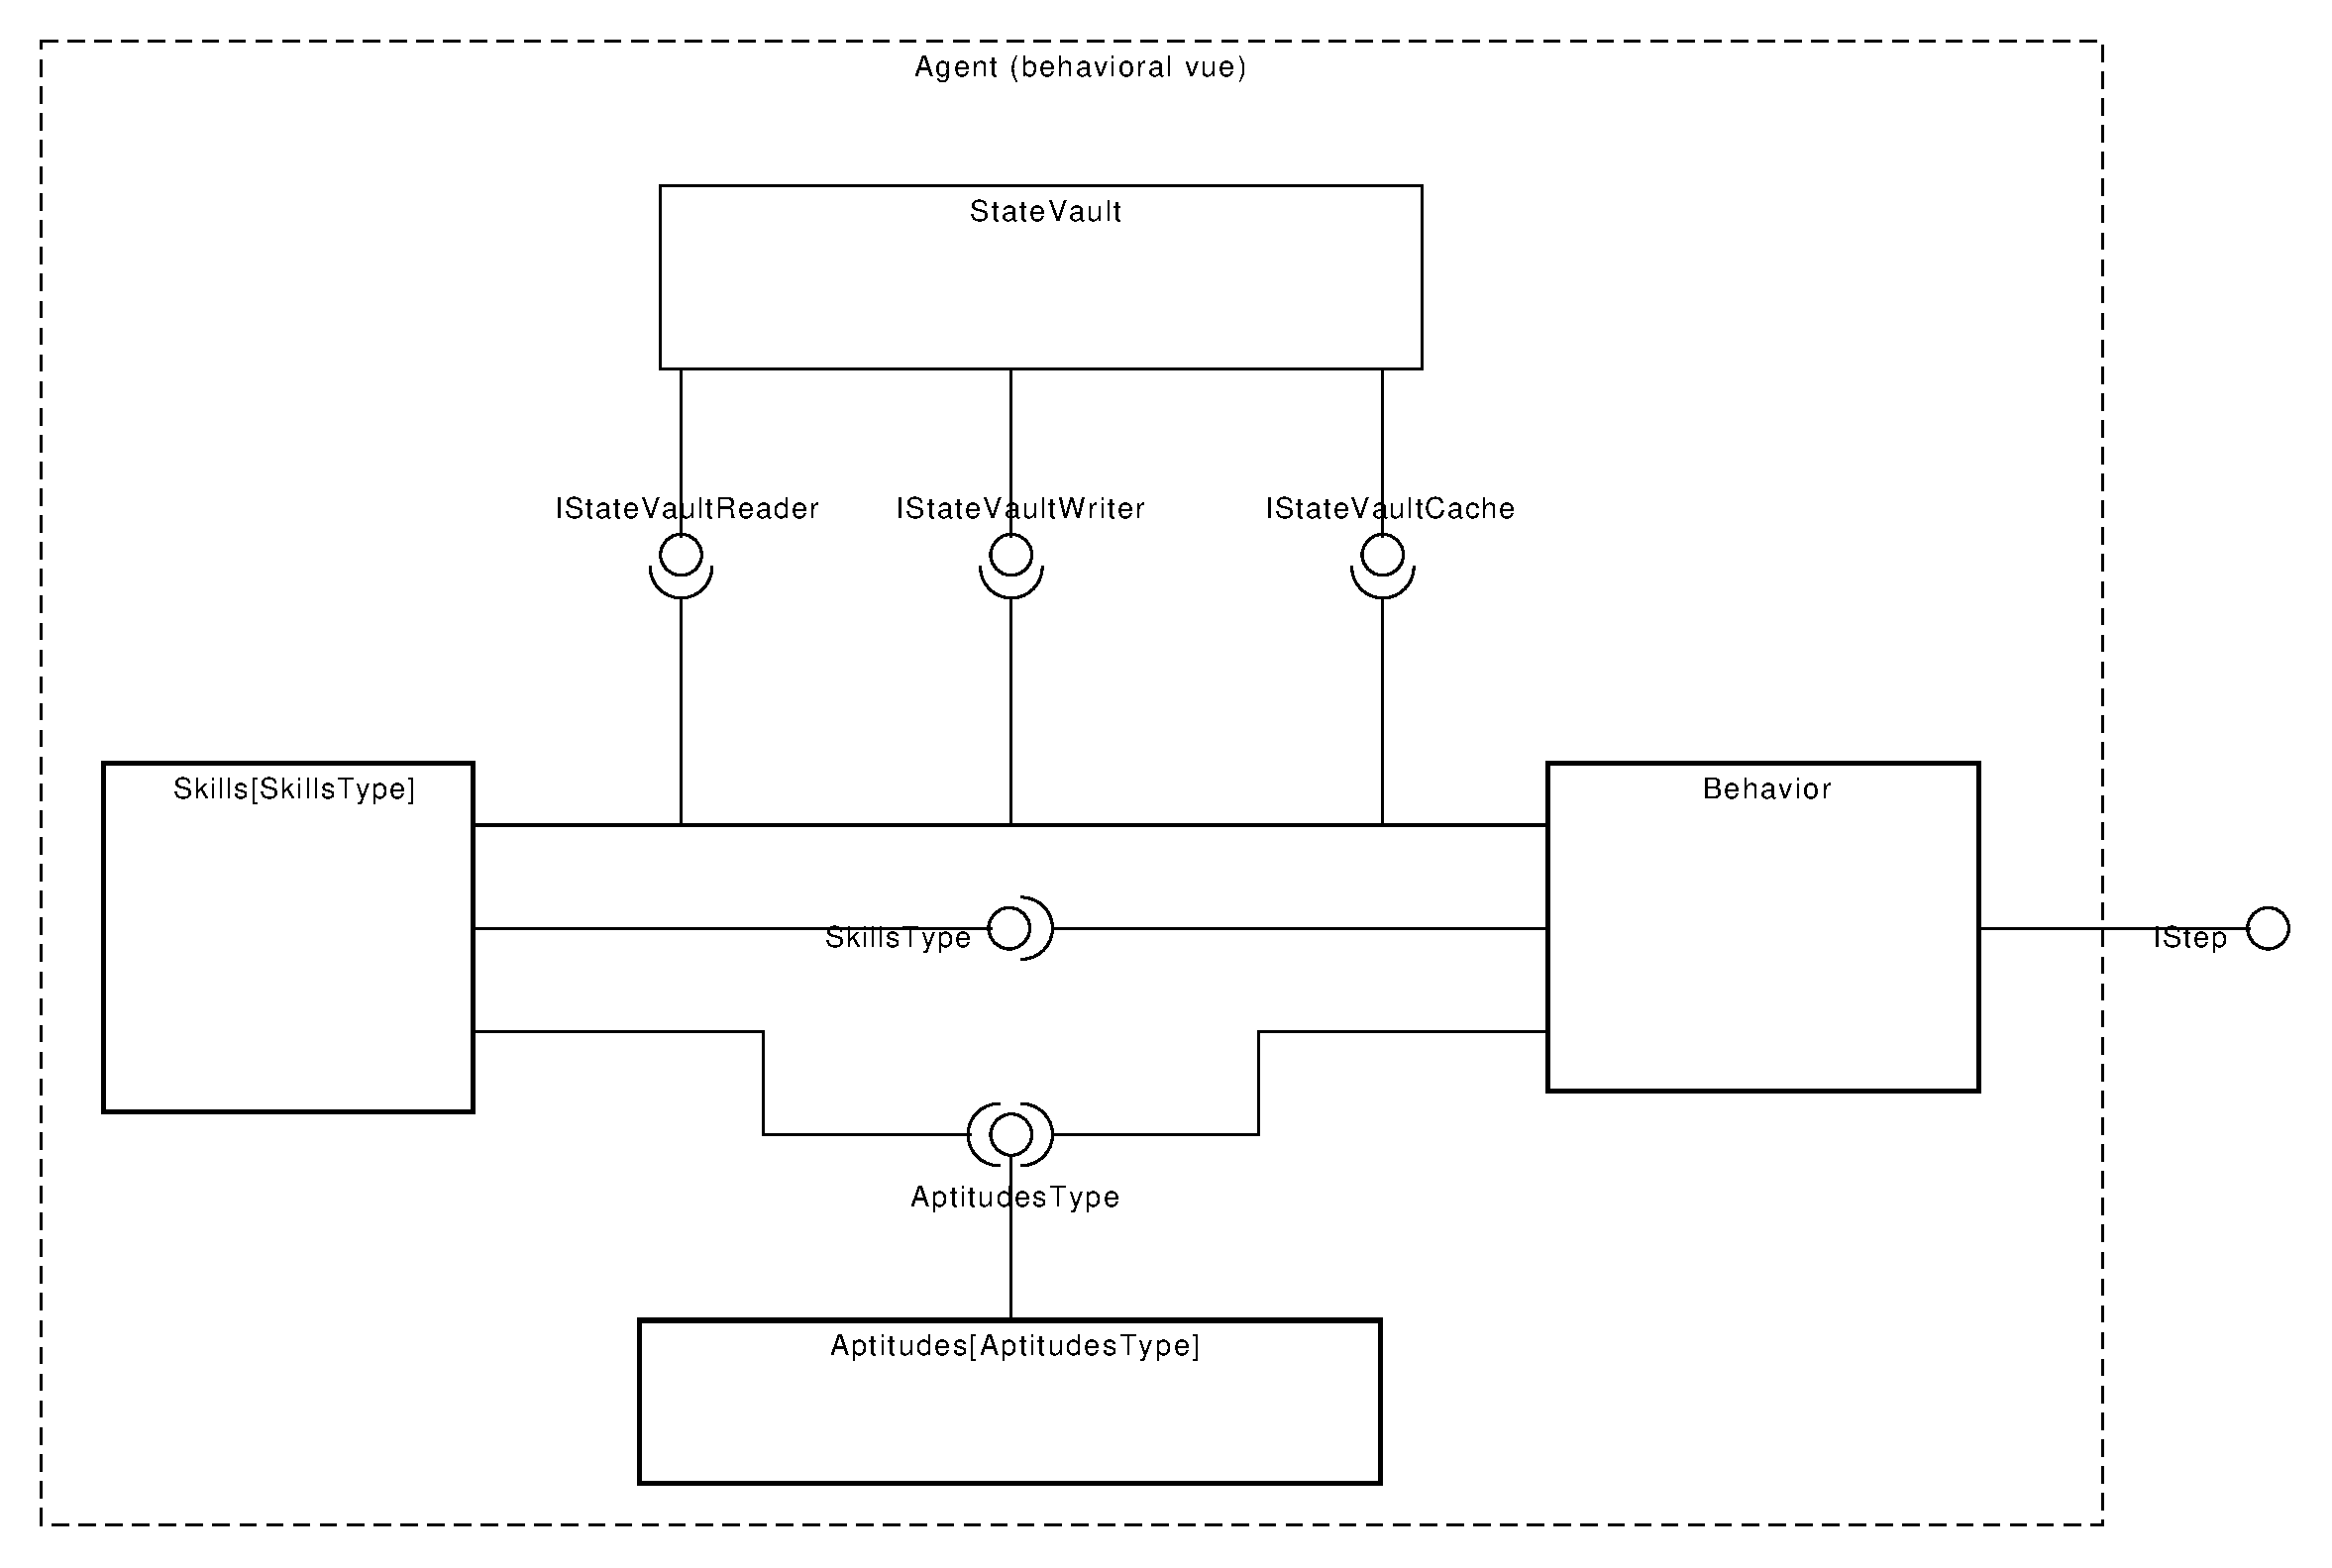
\includegraphics[width=0.6\paperwidth]{ID4CS_Speadl_behav}
\caption{Agent Architecture - Behavior view.}
\label{Arch-behavior}
\end{figure}

The \emph{Behavior} component contains the rules which dictate the behavior of the agent. This component can be seen as the [[chef d'orchestre]] of the architecture. This component exposes to the outside of the environment the \emph{Step} port, which is used to make the agent execute a step. During a step the \emph{Behavior} component executes the agent rules. These rules will in return make use of the others components of the agent.

[[DIRE QUE LES RULES ONT ETE PRESENTEES DANS UN CHAPITRE PRECEDENT]]

The \emph{State Vault} contains the state of the agent. It is used by the components which need to save and read some state variables. Centralizing all the states variables into one component provides several benefits. First it is easier to save and restore the state of the agent, as we just need to save the content of the vault. It is also simple to share some data between components, as long as these components have access to the vault. And it is easy to provide a view of the agent state by just reading the State Vault.
This approach has however several drawbacks. It adds some boilerplate code when writing code using the agent state, as we need to explicitly read the value from the vault (and possibly store it to the vault if modified). It make more difficult to track side-effects, as it is not obvious to know which component uses which value. At last there is no way to strictly enforce that components only use the State Vault for storing state values, as neither Java nor MAY can provide such guarantee.

The \emph{Skills} component contains the skills of the agents. Skills are [[skill definition]]. Each agent type has its own skills set, and skills can require to read and modify the agent state (thus the link between this component and the \emph{State Vault}).
Some skills are used directly from the \emph{Behavior} rules but some skills can also be used by others skills.
Some examples of skills are: for a \emph{Variable agent}, the capability to change its value based on the requests it received and its old value. For a model agent, the capability to translate a request it received to change one of its outputs into a set of requests to send to its inputs.

[[PARLER DU FAIT QUE LES SKILLS ONT LEUR PROPRE ARCHITECTURE ??]]

The \emph{Aptitudes} component contains the aptitudes accessible to the agents. Aptitudes are [[Aptitude definition]]. Unlike skills, aptitudes are general capabilities which do not rely on the state of the agent. Consequently, all agent types have access to the same aptitudes, and there is only one implementation of the \emph{Aptitudes} component.
Some aptitudes are used directly from the \emph{Behavior} rules but some aptitudes can also be used by skills or others aptitudes.
Some examples of aptitudes are: ordering a set of requests from the most to the least important. Make some manipulations on the exchanged values (adding, calculate the norm etc.).

\subsection{Communication}

The \emph{communication} view (\figurename \ref{Arch-comm}) presents the components related to the communication capabilities of the agent. 

\begin{figure}
\centering
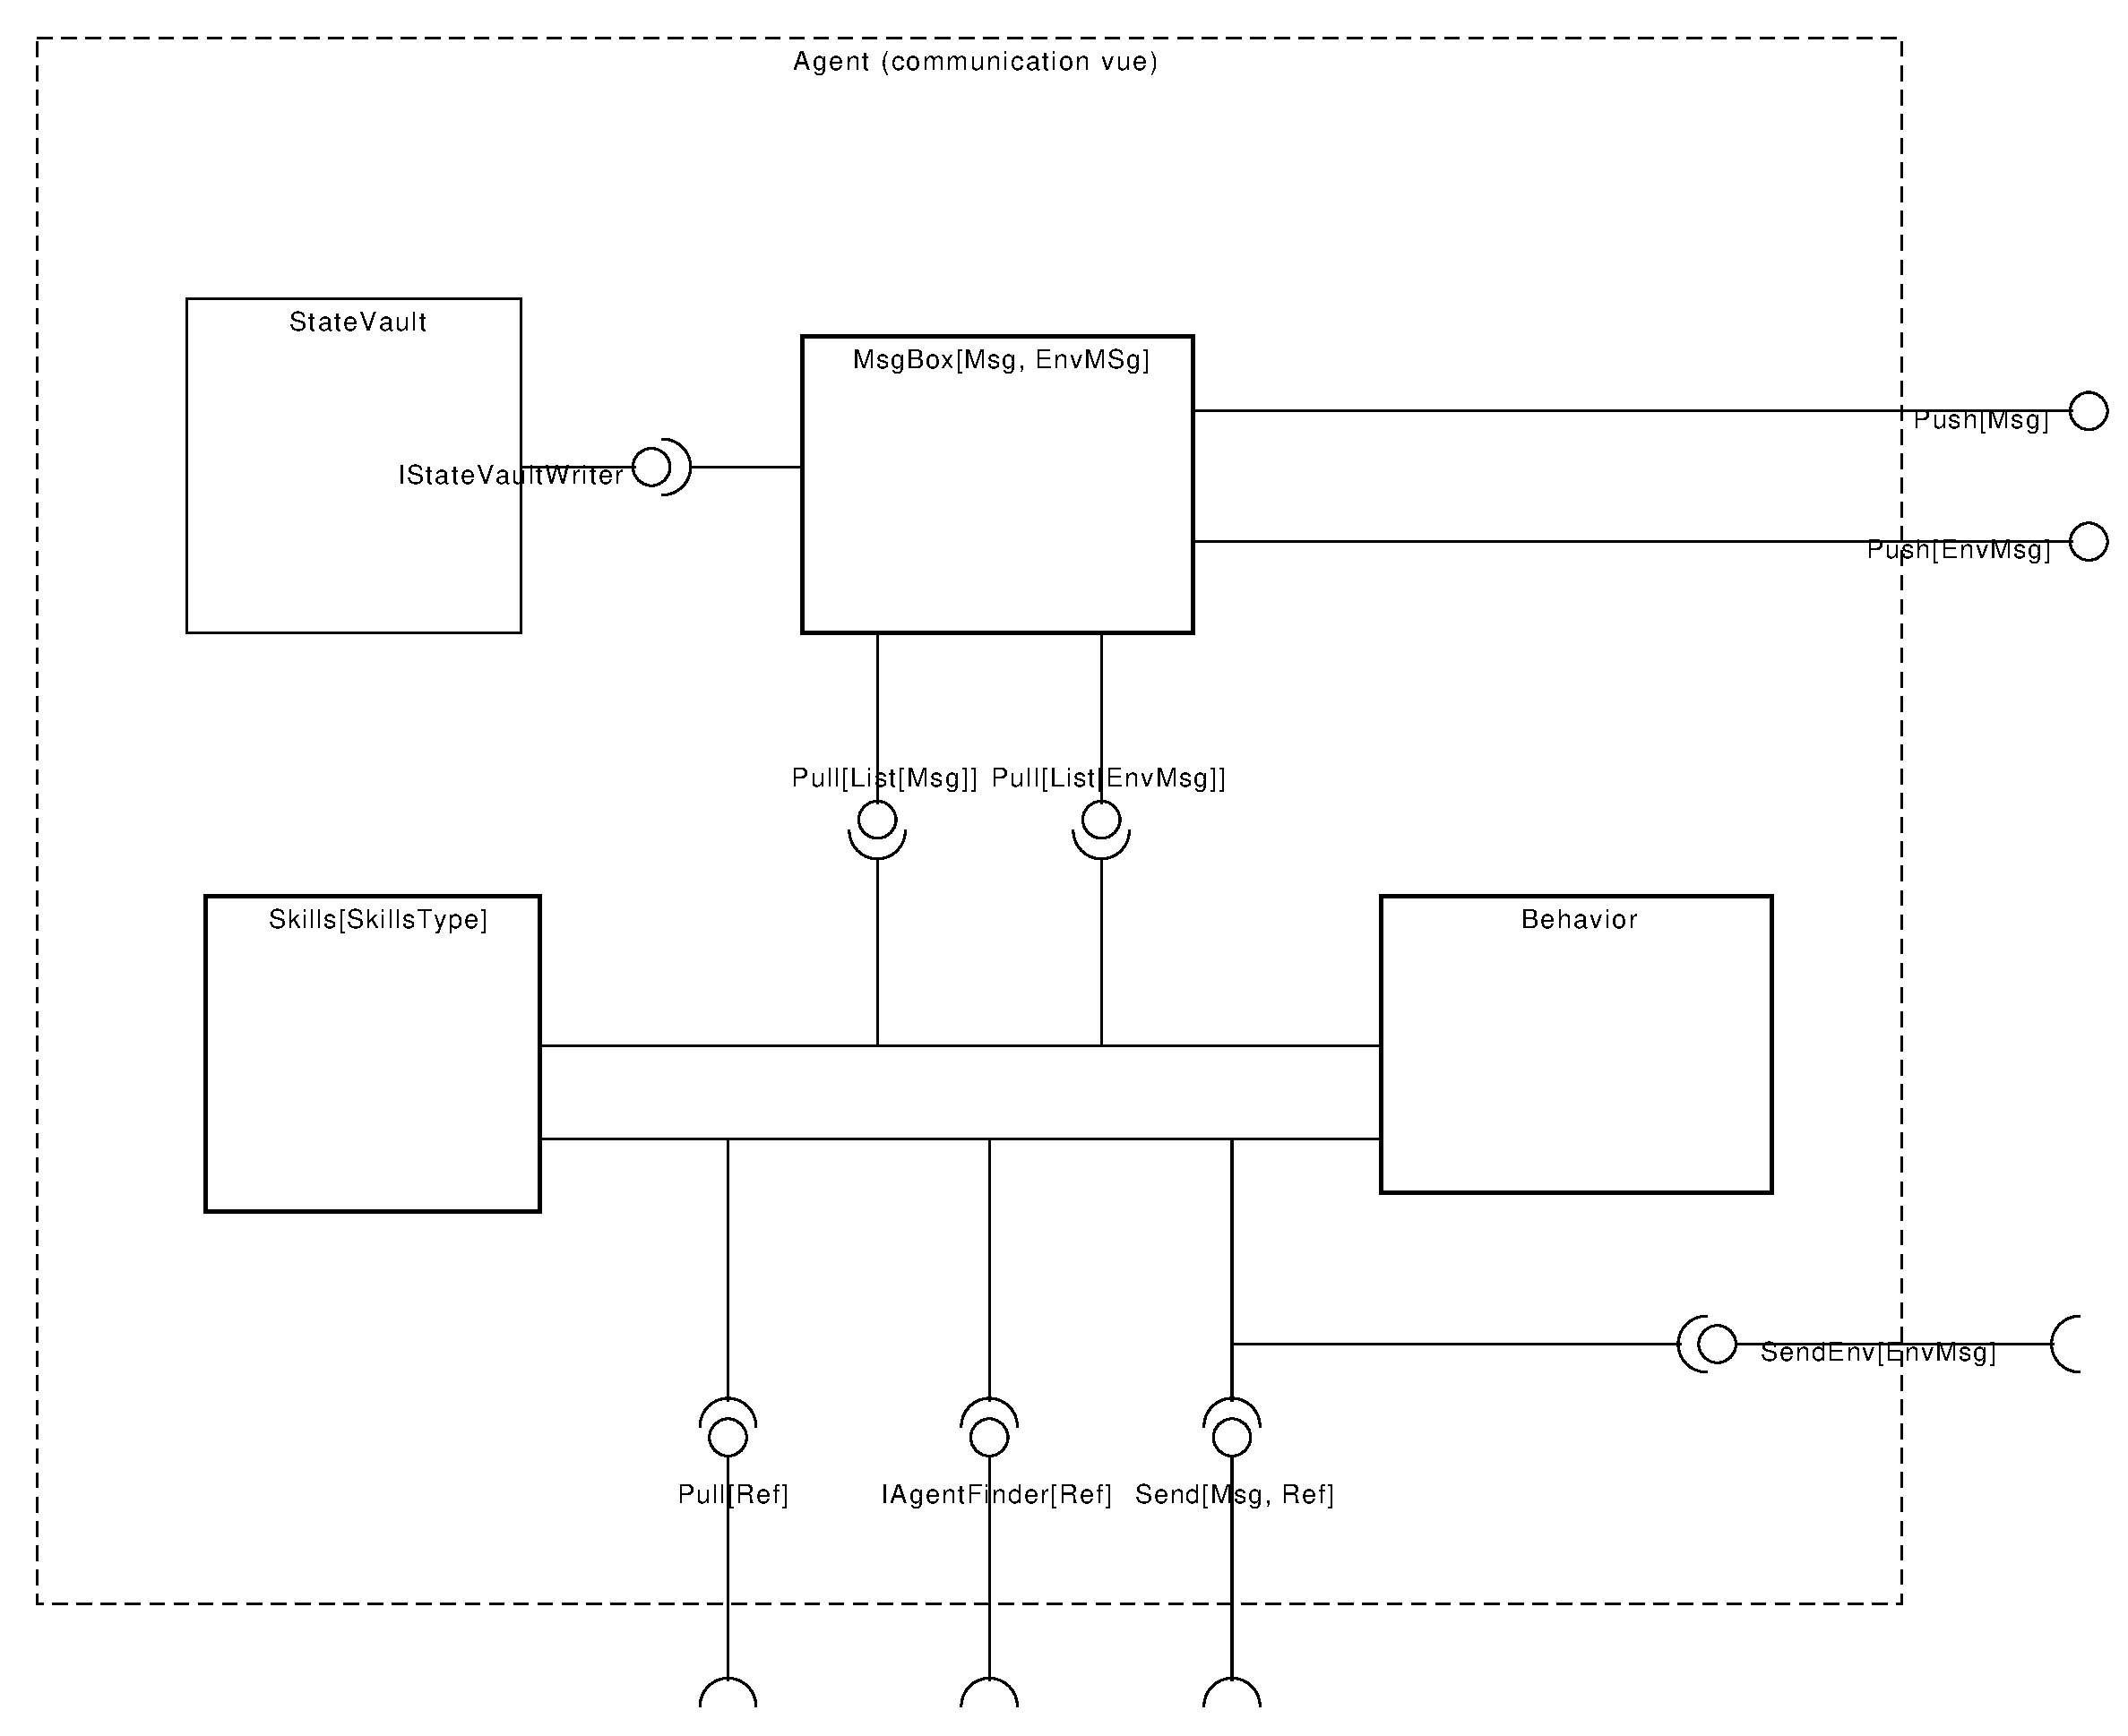
\includegraphics[width=0.6\paperwidth]{ID4CS_Speadl_comm}
\caption{Agent Architecture - Communication view.}
\label{Arch-comm}
\end{figure}

This view contains the new component \emph{Message Box}, which contains the messages sent to the agent. The \emph{Message Box} stores the messages into the \emph{State Vault} and provides a direct access to the \emph{Skills} and {Behavior} components.

This figure presents several ports which need to be provided from the environment to the agent. The environment must give an unique \emph{Reference} to the agent, which will be used by the others agent to communicate with it. The environment must also provides some ports to communicate with the others agents and outside of the system.
[[PARLER DE L'AGENT FINDER ??]]

\subsection{Monitoring}

The \emph{monitoring} view (\figurename \ref{Arch-monitor}) presents the components related to the monitoring of the agent. 

The new component introduced in this view is the \emph{Monitor}. The \emph{Monitor} provides to the environment to ports. The first port is used for external monitoring interfaces to subscribe to be informed of changes in the state of the agent. The second is used to provide informations concerning changes of a specific part of the agent. Thus, an external monitoring interface can subscribe to be notified when the state of the agent changed using the first port, and then use the second port to access to the specific informations it want to monitor.

In order to provide its capabilities, the monitor agent need to be informed by the \emph{Behavior} component before and after each step, to read and compare the monitored informations into the \emph{State Vault}.

\begin{figure}
\centering
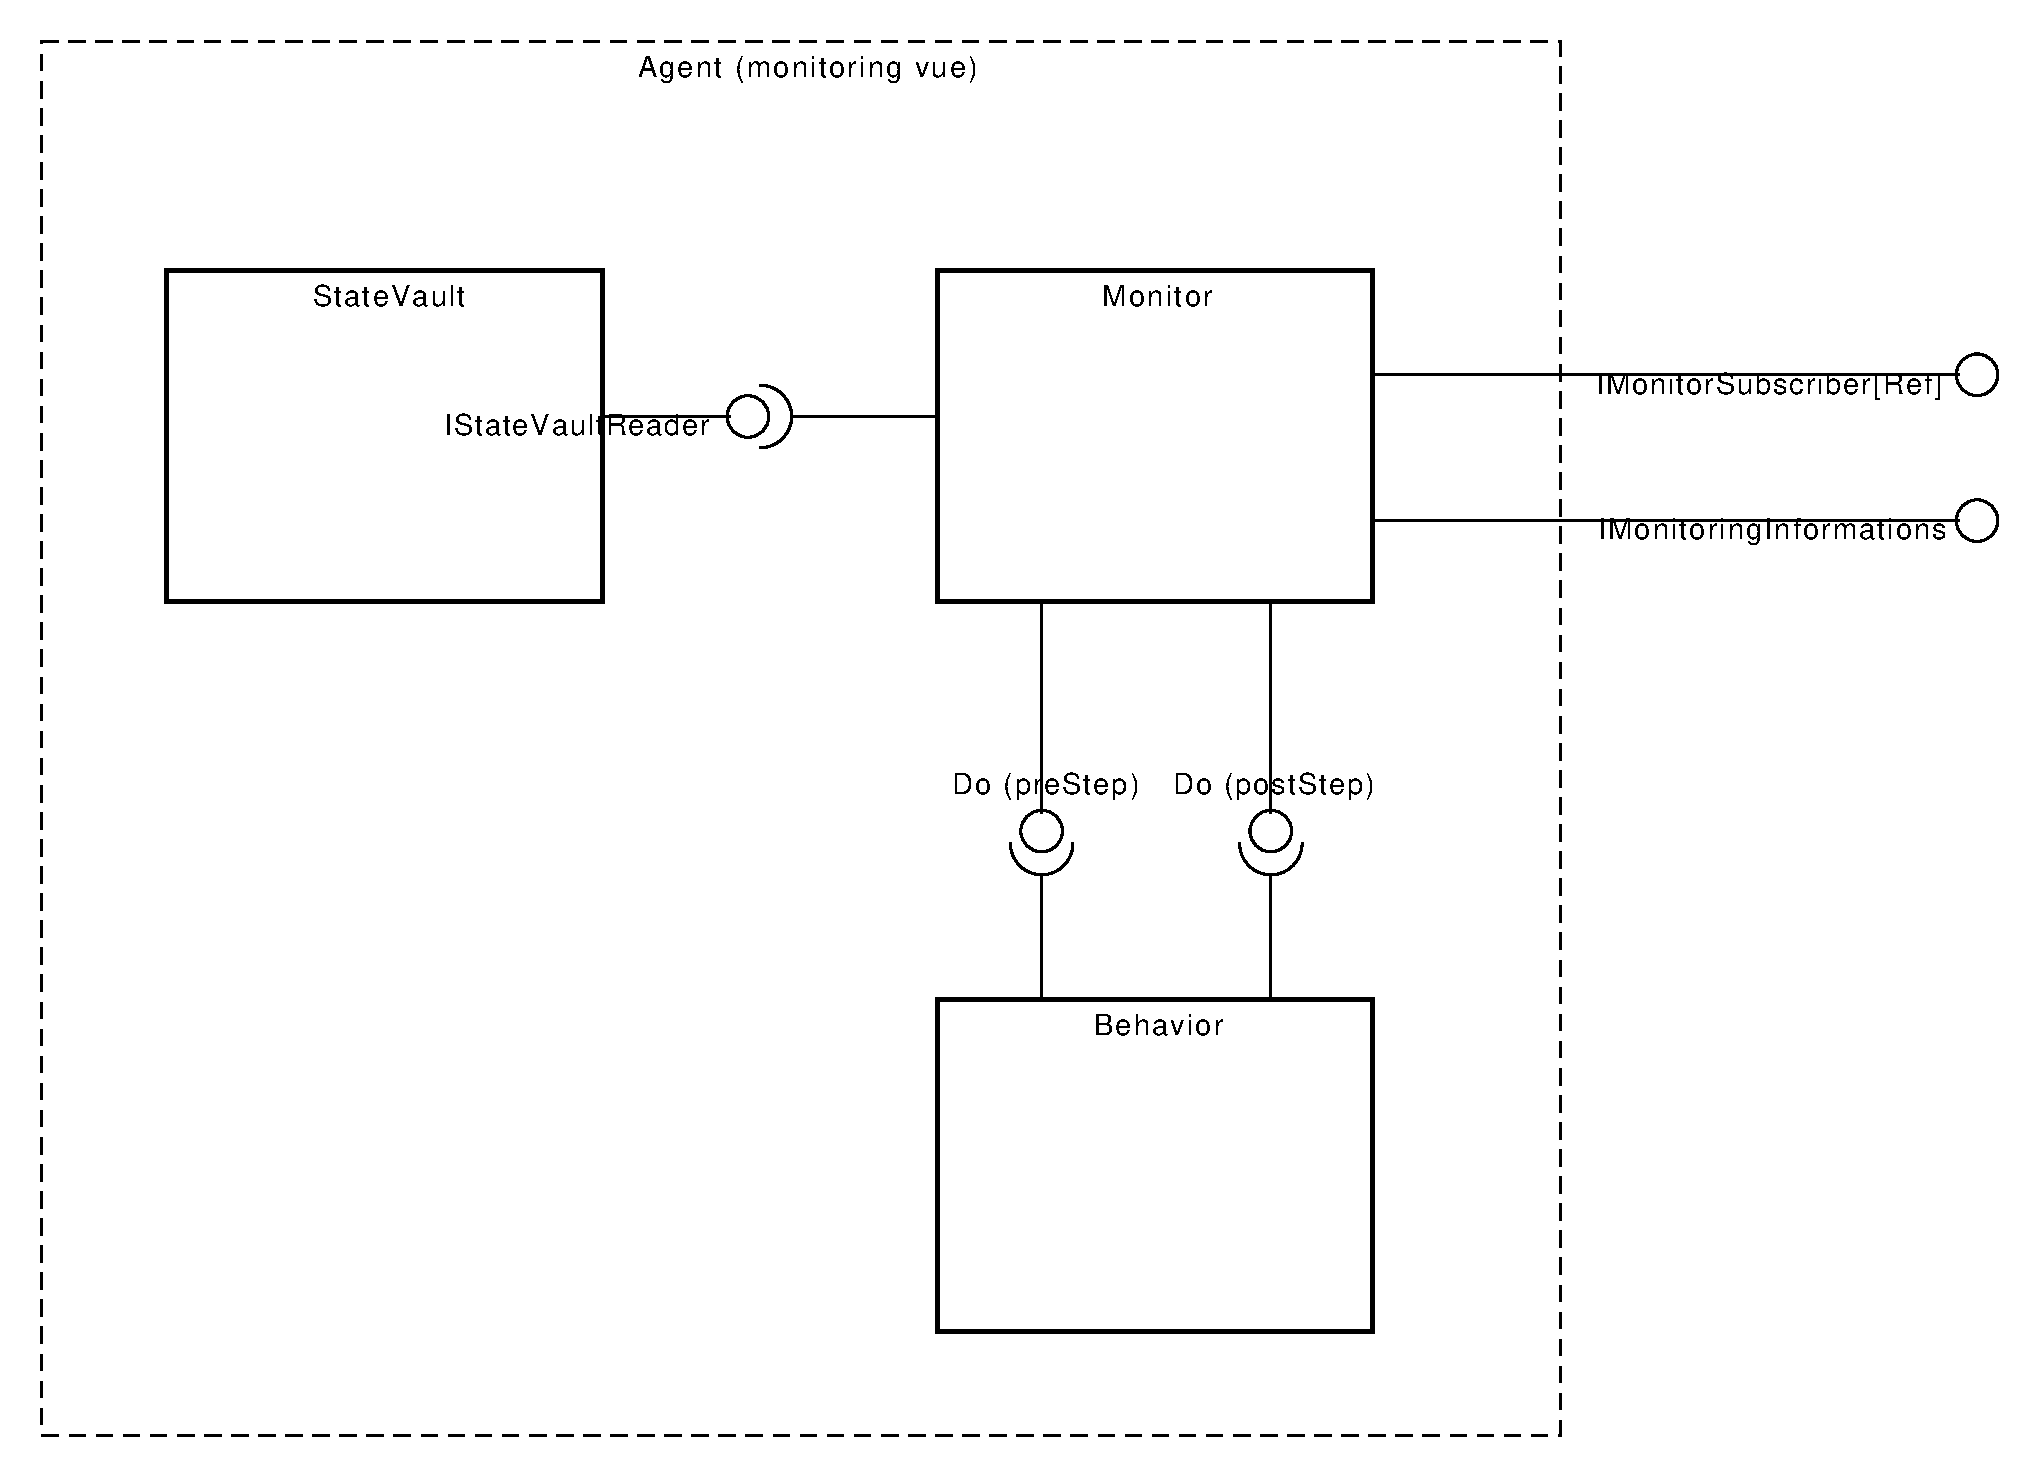
\includegraphics[width=0.6\paperwidth]{ID4CS_Speadl_monitoring}
\caption{Agent Architecture - Monitoring view.}
\label{Arch-monitor}
\end{figure}

\section{MAS Architecture}

\section{Integration into the prototype}

[[OSGI and EMF]]

\chapter{Analysis - Collective Solving Patterns}

\part{Design, Implementation and Extending the AMAS4Opt Building Blocks}

The work presented in this thesis is part of the ongoing ID4CS project. ID4CS (\emph{Integrated Design for Complex Systems}) is funded by the French \emph{Agence Nationale de la Recherche} (National Research Agency)\footnote{COSINUS program, ANR-09-
COSI-005 reference} and involves nine partners, both from the academic and industrial work. The goal of the ID4CS project is to use the MAS approach to provide new tools for the design of complex systems. Our industrial partners, Airbus and Snecma, are involved in aeronautical design, and are thus fully concerned by the problematic of complex continuous optimization for system design.

For this reason, one of our goals was not only to propose a new approach for continuous optimization, but also to put this approach in practice by integrating it into a working prototype which could be used by our partners. To this end we worked with our partners, including optimization specialists and software development experts, to propose such a tool, basing ourselves upon the ADELFE method. This method aims to guide the development of AMAS-based softwares from high level user requirements to the implementation nuts and bolts. Using ADELFE we made a comprehensive analysis of the domain and actors involved in the use of such a tool.

We also use the design tools provided with ADELFE to instantiate our MAS and integrate it into the prototype, among which the recent MAY framework. The goal of MAY is to provide suitable abstractions as well as reusable software components for the development of agents and multi-agents systems. We contributed to the enrichment of its components library by developing a general and modular agent architecture consistent with the AMAS theory, notably by proposing a \emph{modular skill stack principle}, where different skills can be composed to address specific requirements.

While such work could seem to concern software engineering experts more than artificial intelligence specialists, we will see how existing MAS oriented methods such as ADELFE are still too high-level to be successfully directly applied to any domain (and more so to continuous optimization) without an important agent expertise and extensive research work. We will detail how the scientific work we produced and presented in the previous part, especially the identification of various NCSs and the mechanisms to solve them, can be generalized into \enquote{building blocks}. These \emph{building blocks} could then be reused to guide the design of other MAS in the domain of problem solving. This work places itself into a more general effort to provide a general reusable toolbox for assisting non experts in applying AMAS to the domain of optimization, under the name \emph{AMAS4Opt} (AMAS for Optimization).

\chapter{ADELFE and MAY Architecture}\label{ADELFE_chapter}

\section{Overview of ADELFE}

In section \ref{AMAS-ADELFE}, we succinctly presented ADELFE\footnote{\url{http:/www.irit.fr/ADELFE/}}, the method which has been proposed for the design of AMAS. In this chapter we get back in more details about this method and what benefits it provided for the design of our system. 

ADELFE is a method devoted to software engineering of adaptive multi-agent systems. It was initiated by a French government funded project lead by IRIT (see \url{http://irit.fr/ADELFE-Project} for details) and has been continuously enhanced since. Like previously said, the name \enquote{ADELFE} is the French acronym for \enquote{toolkit to develop software with emergent functionality} (\textit{Atelier pour le DEveloppement de Logiciels à Fonctionnalité Emergente}).

The ADELFE method in itself is based on the Rational Unifed Process (RUP) and is defined following the Software Process Engineering Meta-Model (SPEM) \cite{PiGl2004.1,BeCaGlPi2005.1}. Since its revision \cite{Ro2008.3}, it is composed of five \emph{Work Definitions} ($WD$), themselves decomposed in several \emph{activities} making use of UML as well as the AMAS-ML and muADL languages. An overview of the method is shown on \figurename{} \ref{ADELFE_phases}.

\begin{figure}
\centering
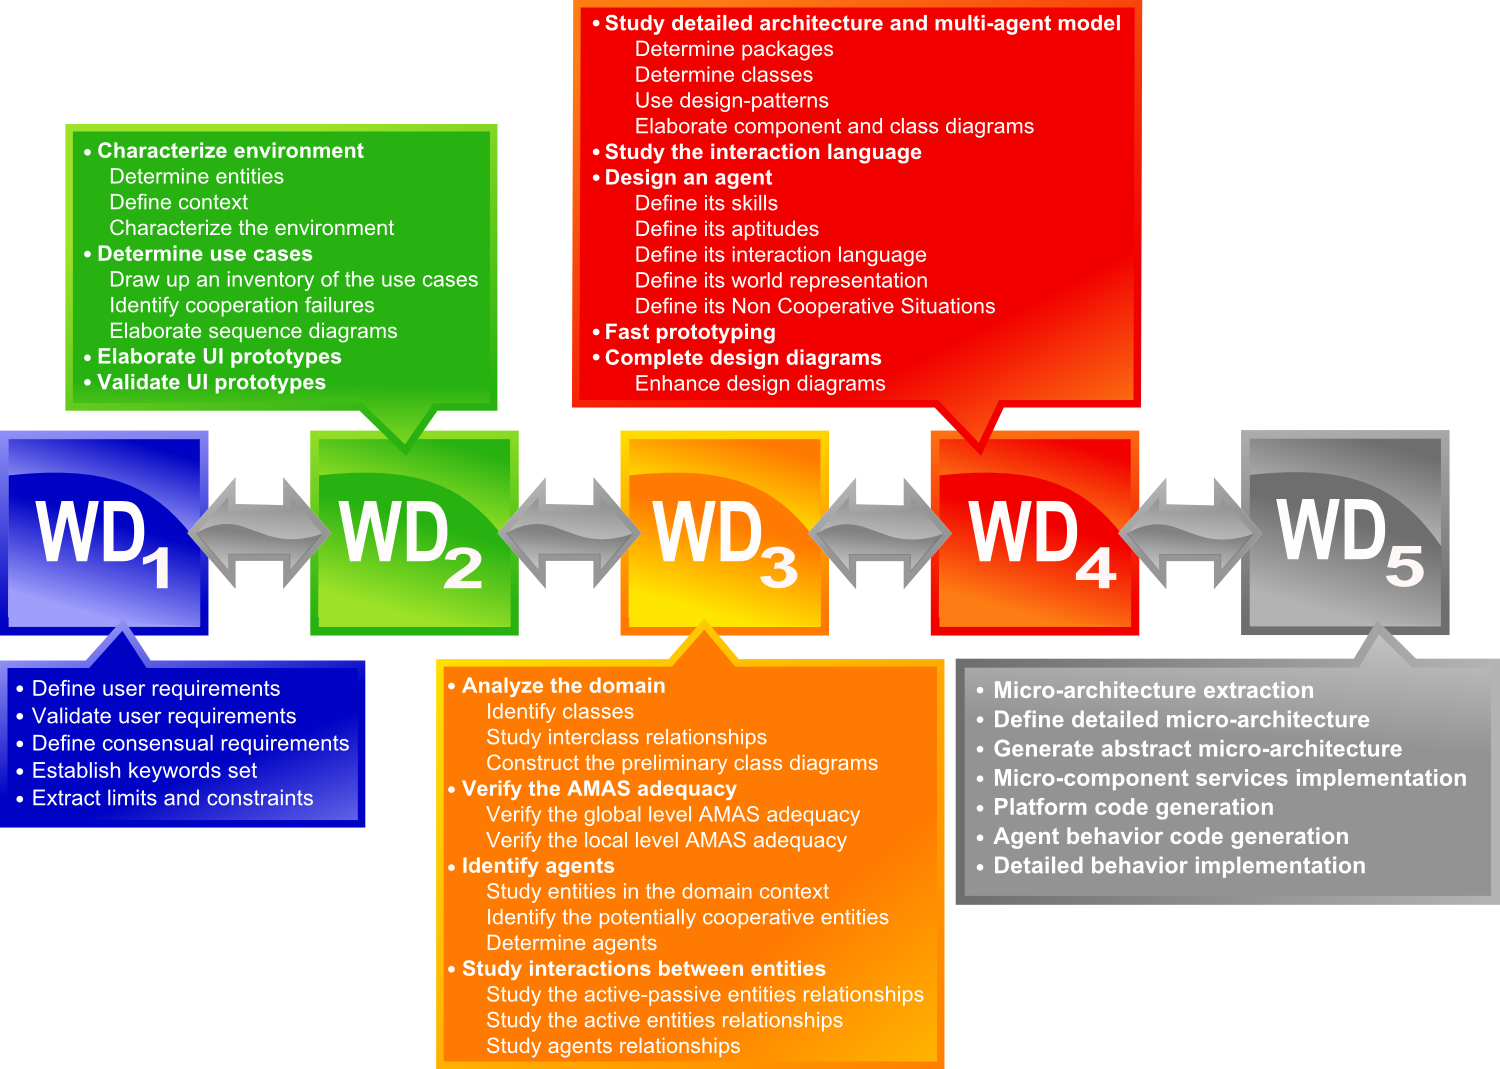
\includegraphics[width=\textwidth]{AdelfePhases}
\caption{Overview of the ADELFE Method.}\label{ADELFE_phases}
\end{figure}

In regard of the RUP, ADELFE adds supplementary activities and roles which are specific to its approach for the design of AMAS compliant software.\\
The final requirement study ($WD_2$), was complemented with activities 6 and 7-2 concerning the characterization of the system environment and the identification of cooperation failures during the determining of the use cases. During the analysis ($WD_3$), additional activities 11 and 12 respectively check for the adequacy of AMAS to the problem and identify the agents involved in the system being built, while activity 13 is complemented with a step concerning the study of the relationships between agents. During the design ($WD_4$), activities 15 et 16 concerns the design of the system and the agents, while activity 17 concerning fast prototyping was added in order to be able to quickly test the proposed behavior of the agents. The development phase ($WD5$) concerns the architecture and the implementation of the agents and the system.

\section{Applying ADELFE for the Design of a Continuous Optimization Tool}

Based on the guidelines of the ADELFE methodology we defined the requirements of the tool we proposed to develop. The following functionalities were identified:
\begin{compactitem}
\item Our tool will allow users to solve multidisciplinary optimization problems.
\item The user will be able to load disciplinary models into the tool, express some constraints and objectives on these models and then use and interact with the tool to solve the defined problem.
\item Our tool will be reusable from one optimization problem to another in different application domains and will be a generic tool.
\item The user will be able to express uncertainties on some parts of the models or input variables.
\item The resolution will take into account these uncertainties.
\item The tool will be able to integrate well-known optimization techniques, and will allow the user to add new techniques to use during solving. The tool will also be able to interact with others optimization tools to ease the optimization process.

\item The user will be able (at runtime):
	\begin{compactitem}
	\item to monitor the system activity,
	\item to observe time history qualitative indicators,
	\item to adjust its parameters.
	\end{compactitem}
\end{compactitem}

\begin{figure}
\centering
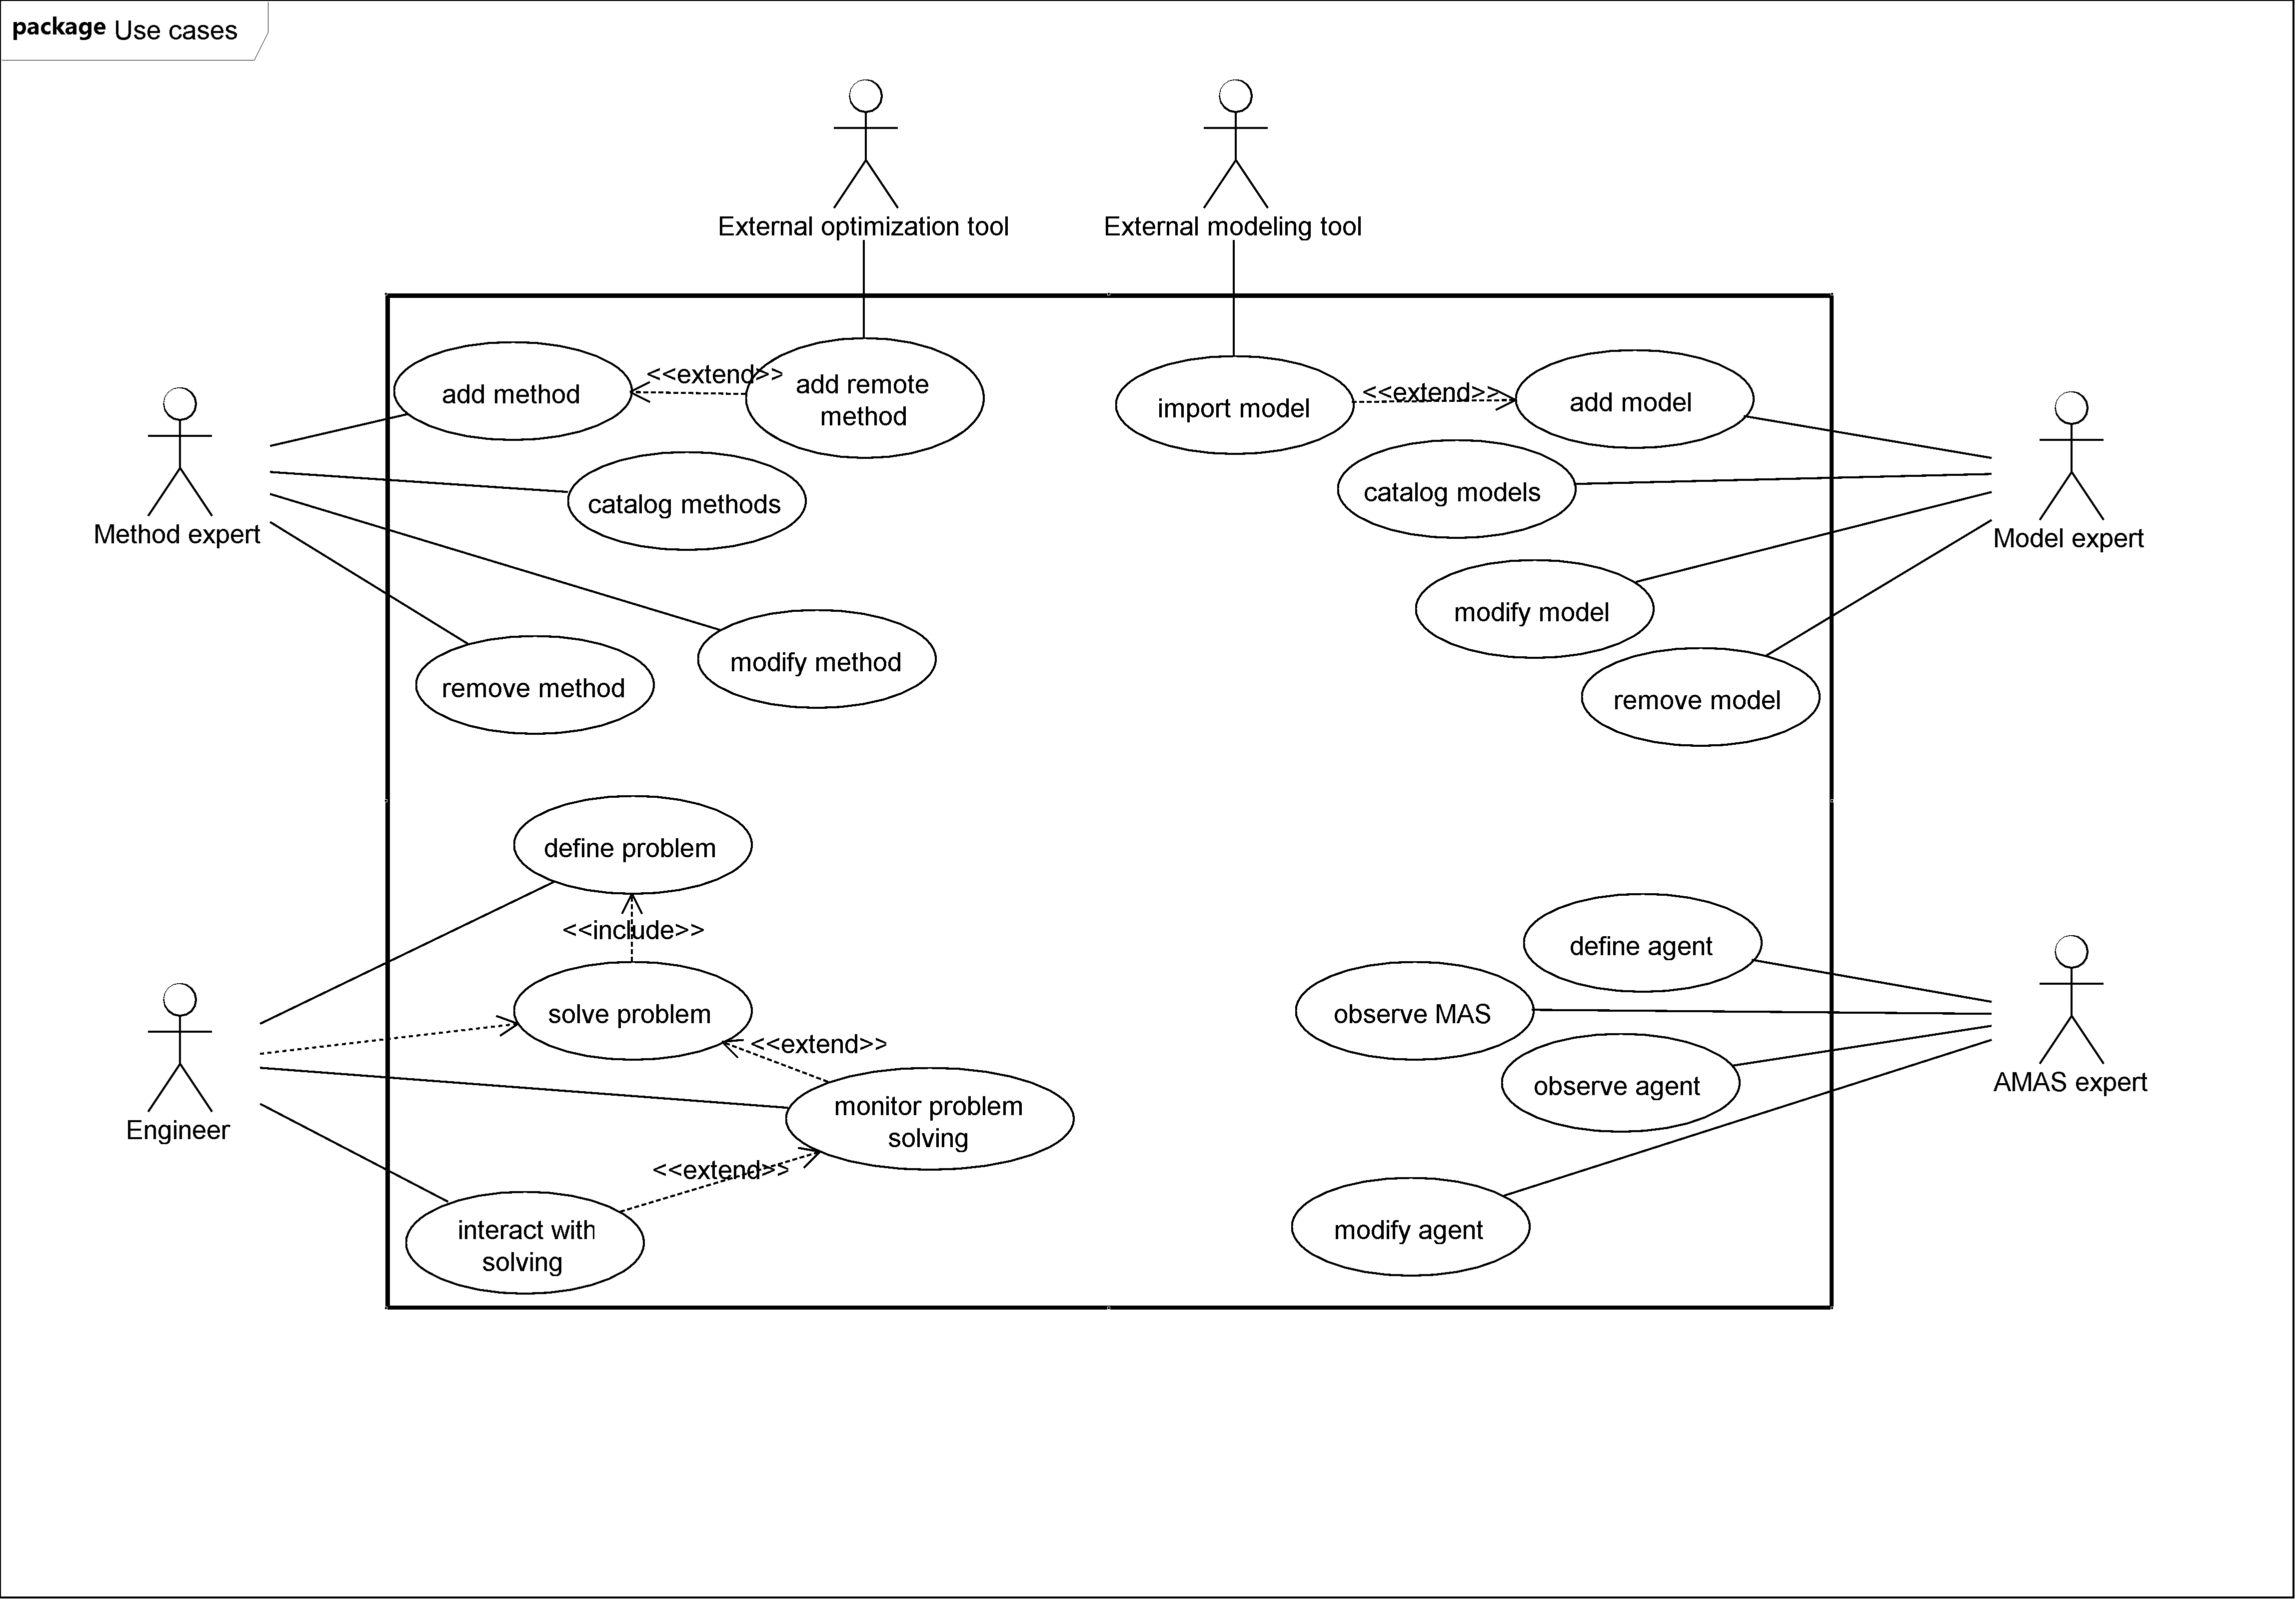
\includegraphics[width= \textwidth]{Use_cases}
\caption{Actors and use cases identified during requirements studies for ID4CS.}\label{Use_cases}
\end{figure}

Several entities interacting with the tool were also identified. The \emph{Method expert} adds new optimization methods into the system. The expert field can be optimization methods (classic methods, AMAS methods ...) or uncertainties. The \emph{Model expert} adds new models into the system. The role of the \emph{Engineer} is to use the different elements defined by the other experts to define new problem for the system to solve and to monitor the functioning of the system. At last, the \emph{AMAS expert} has to define and tune the agents of the system. The system should also be able to integrate with external optimization and modeling tool, in order to accommodate the existing workflow and constraints of the users.

The different use cases which were identified for each of these entities are presented in \figurename{} \ref{Use_cases}.

The domain analysis (activity 10) roughly correspond to the work we provided in \ref{modeling}, as this activity correspond to the study of the application domain in interaction with the domain experts. The domain modeling roughly corresponds to an extended version of NDMO, with some additions and adjustments regarding the expected functionalities of the prototype. These adjustments concerns mainly the introduction of the \emph{workspace} and \emph{project} concepts, which allows the designer to organized its work, as well as the introduction of the external optimizer and uncertainties propagators as domain entities, in order to provide a more seamless integration of these tools into the prototype.\\
ADELFE then advocates an AMAS adequacy verification (activity 11), in which one checks using a set of questions if AMAS are a relevant solution for the problem to solve. We discussed at length in chapter \ref{AMAS_chapter} the advantages of the AMAS approach. Without much surprise the results of this activity were strongly in favor of using an AMAS solution, as the problem we aim to solve is highly distributed, is not easily solvable by known algorithms, is potentially non-linear and evolving.

The next activities concerned the design of the agents themselves, their interactions, the identification and solving of the Non Cooperative Situations. The work concerning these activities is without much doubt the most difficult, involving in the ADELFE method the participation of an \enquote{agent designer}. Indeed, this part of the ADELFE method stays at a high abstraction level, and we can say without much controversy that the process of designing the agents is still highly exploratory, probably currently more related to a scientific study than to an engineering development. In this regard, our contribution presented in part \ref{MAS4Optim_part} provides the expected answers to these activities.

The last WD of ADELFE corresponds to the design of the agent architecture and implementation using MAY, the component-based framework developed in complement of ADELFE. While such framework aims ultimately to make the process as seamless and automated than possible by providing reusable components, its early state implied once more some exploratory work on our part in order to produce, and in the end contribute to the MAY library with our own produced components. We will now see in the next chapter the architecture we proposed for a modular AMAS agent design.

\section{MAY Agent Architecture}

To implement the MAS, we used the Make Agents Yourself (MAY) framework \cite{No2012.2}. MAY is a component-based framework that automatically generates an implementation of an agent architecture from a given description.

The ADELFE methodology proposes an abstract agent architecture (represented in \figurename{} \ref{AMAS-ML_agent}), which we translated into the MAY architecture description language, SpeADL. In the context of our study, as the agents communicate and interact only by messages passing we could make some simplifications in regard of the original modeling of communications and actions capability of the agents. All our agents use the same AMAS architecture. They are differentiated by specific implementations of the components. For example, \emph{Model} and \emph{Variable} agents will have different implementations of the \emph{Behavior} component.\\
The components of a MAY architecture are connected by \emph{ports}. A port can be though as a service interface, listing a set of available operations. Components expose lists of available and required ports. A component required ports must be linked to available ports provided by other components, satisfying these interfaces.

\begin{figure}
\centering
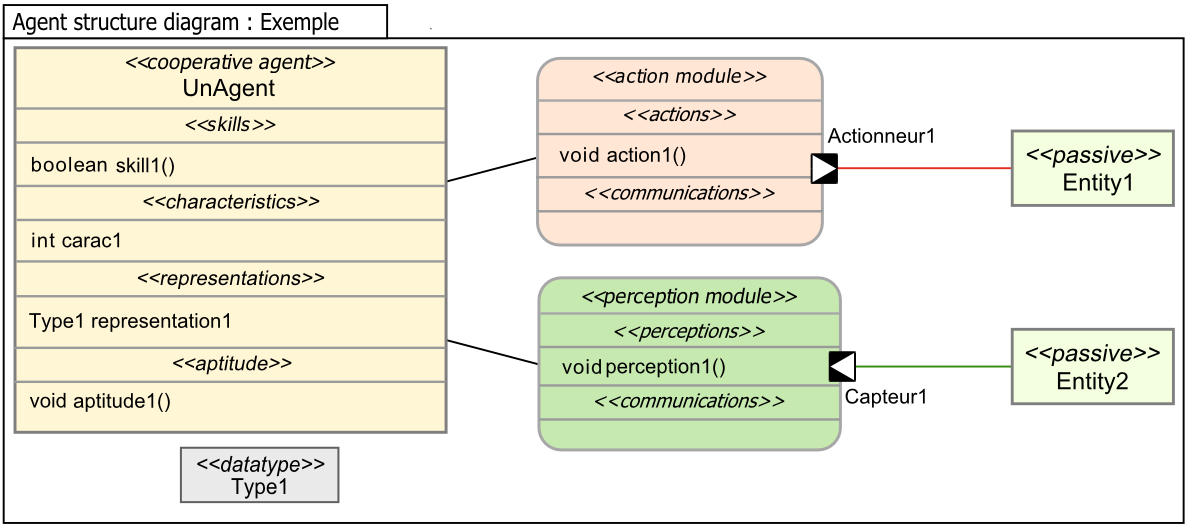
\includegraphics[width=\textwidth]{amasmlAgent}
\caption{AMAS agent architecture (as defined in ADELFE).}\label{AMAS-ML_agent}
\end{figure}

An illustration of this composition mechanism is shown on \figurename{} \ref{Speadl_example}. Two components $A$ and $B$ are present. The component $A$ exposes a port $P$ as available, which is required and used by the component $B$. Consequently, this last component is now able to call the operations declared by $A$ through this port, operations which are supposedly necessary for the good functioning of $B$. The way ports are used to connect otherwise independent components is in this way not too dissimilar to the role interfaces play in the context of \emph{dependency injection} design pattern.

\begin{figure}
\centering
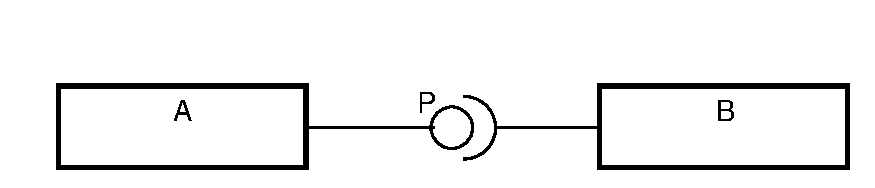
\includegraphics[width=0.4\textwidth]{Speadl_example}
\caption{Example of MAY composition.}\label{Speadl_example}
\end{figure}

For the sake of clarity, the agent architecture is separated in three views: the \emph{behavior}, \emph{communication} and \emph{monitoring} views.

\subsection{Behavior}

The \emph{behavior} view (\figurename{} \ref{Arch-behavior}) contains the components related to the behavior of the agent. 

\begin{figure}
\centering
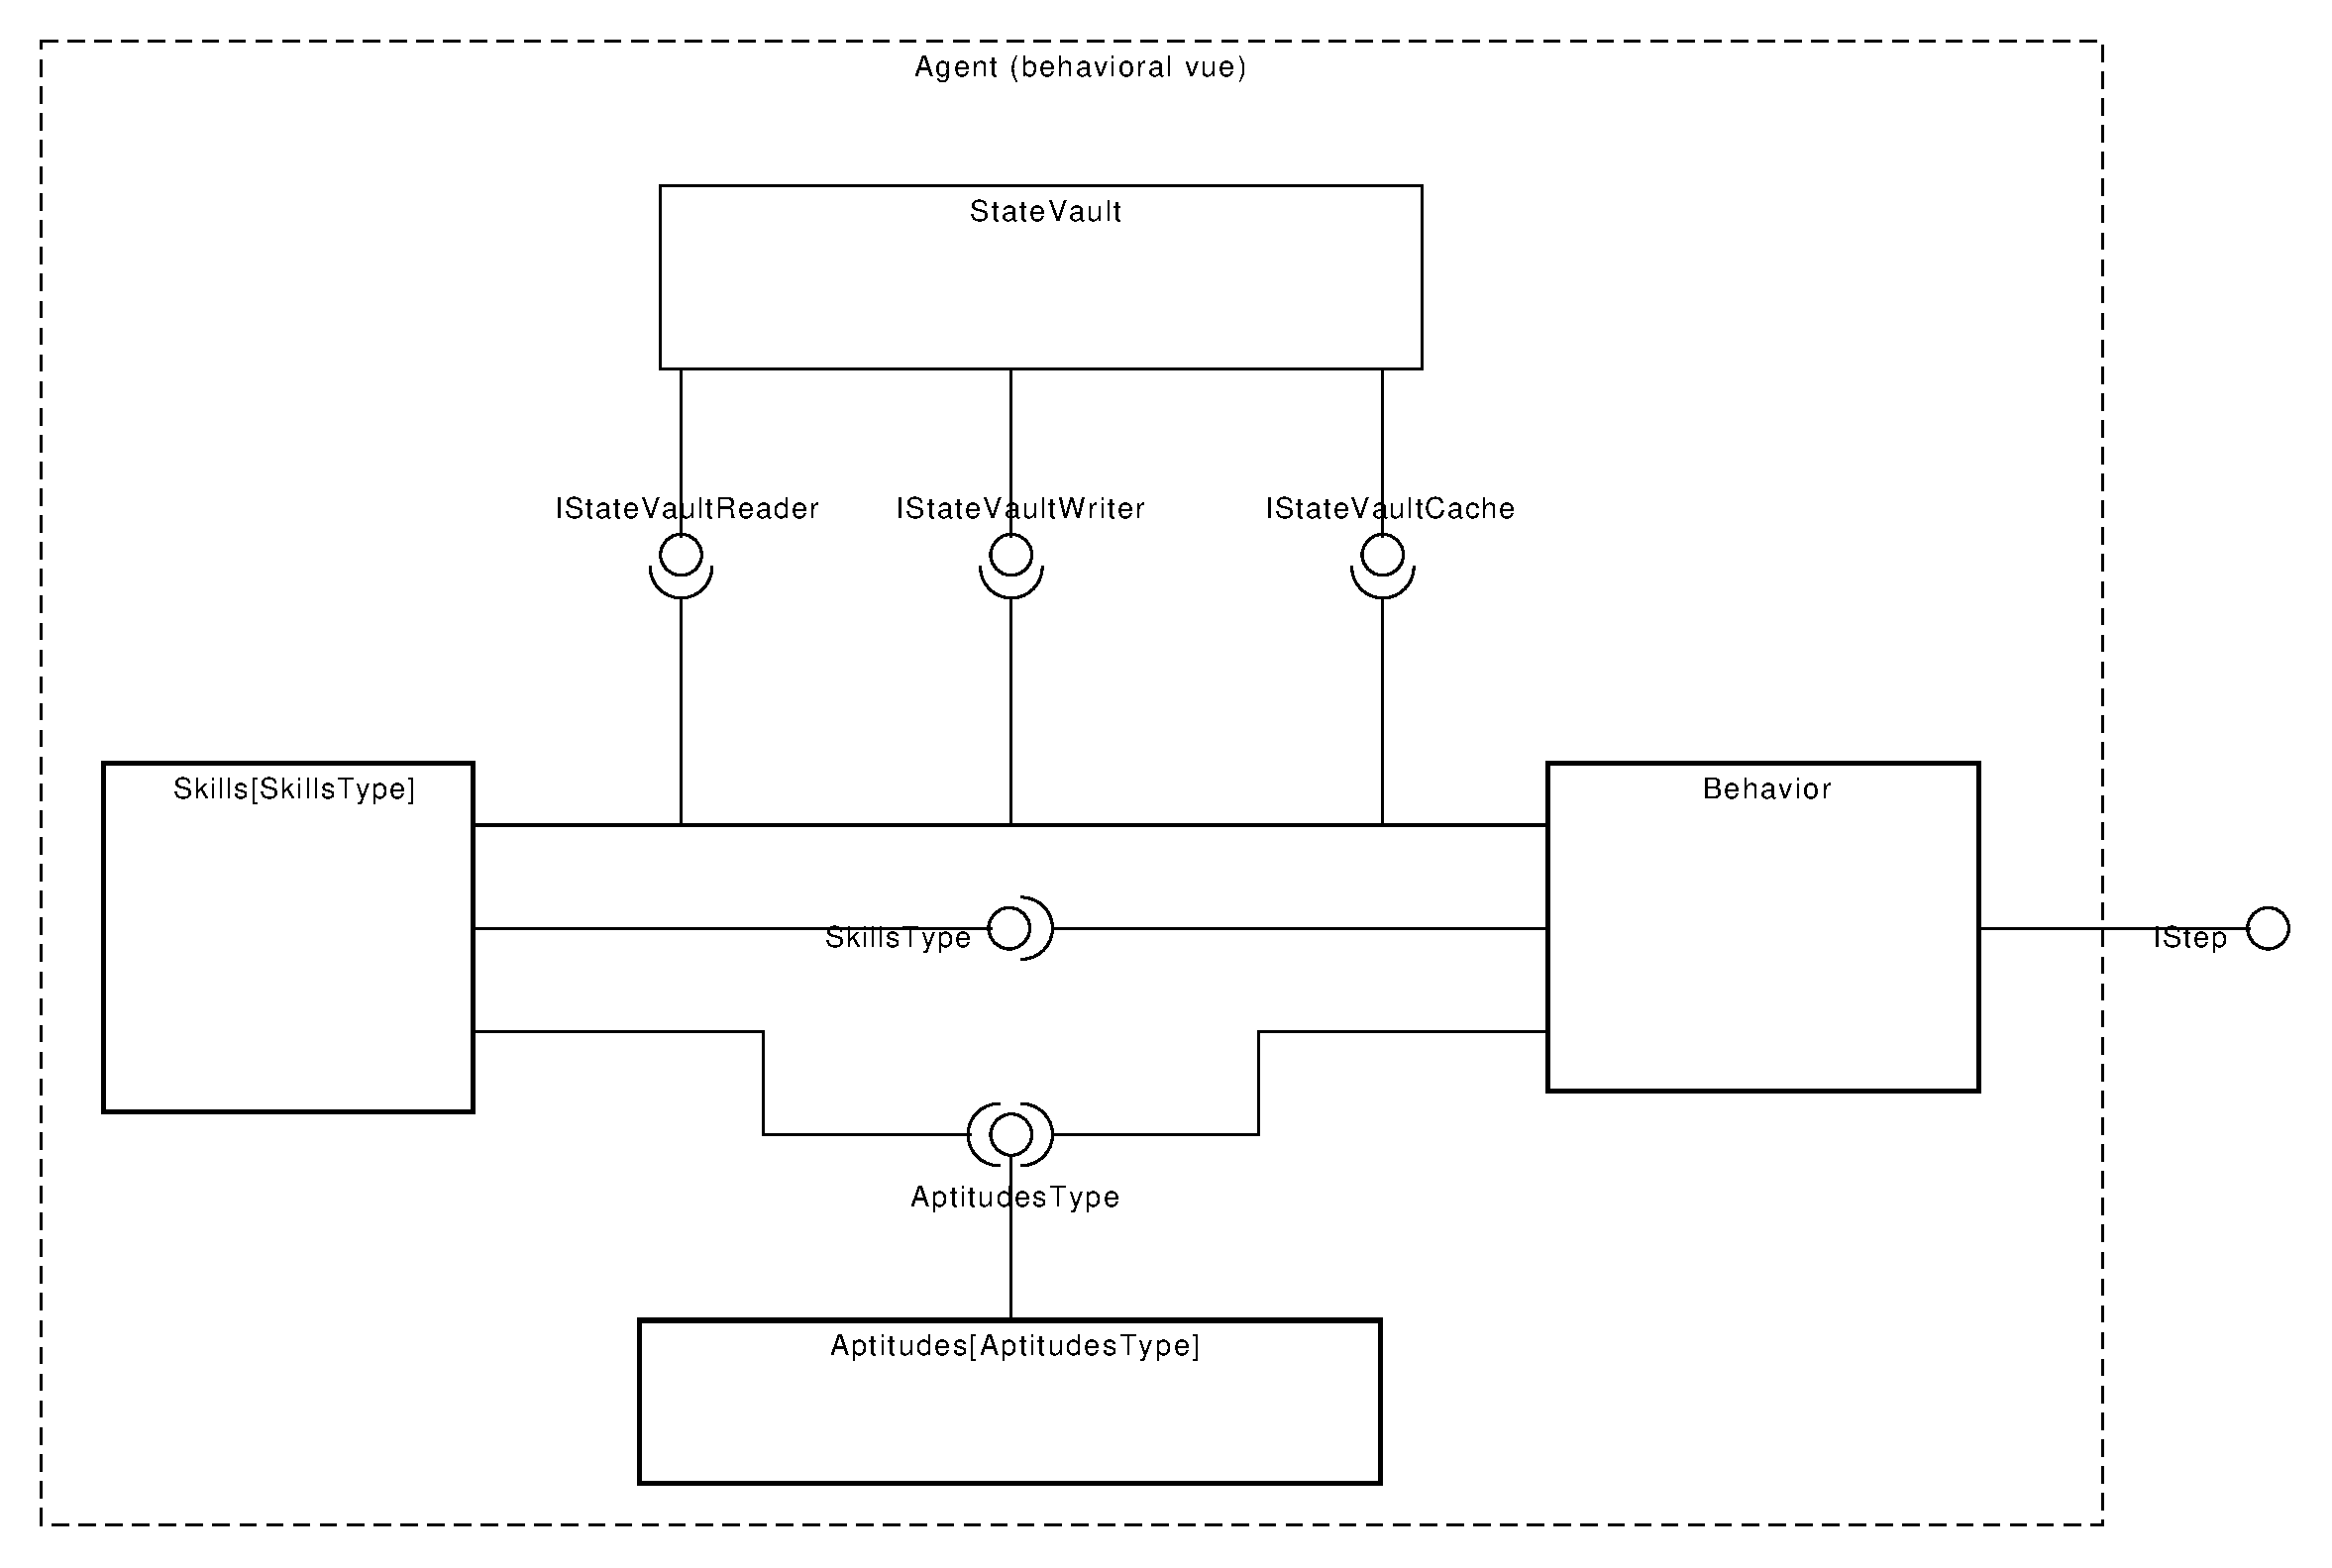
\includegraphics[width=\textwidth]{ID4CS_Speadl_behav}
\caption{Agent Architecture --- Behavior view.}
\label{Arch-behavior}
\end{figure}

The \emph{Behavior} component contains the rules which dictate the behavior of the agent. This component can be seen as orchestrating the architecture. This component exposes to the outside of the environment the \emph{Step} port, which is used to make the agent execute a step. During a step the \emph{Behavior} component executes the agent rules. These rules will in return make use of the other components of the agent. [[RMK MPG: 1 exemple de règles cf 13.1 (??)]]

This behavior component contains the behavioral algorithms presented in chapter \ref{agent_behav_chap}. This component mostly contains the parts regarding the general steps of the agent behavior and making use of the more specialized methods implemented in the \emph{Skills} and \emph{Aptitudes} components (for example, the exact computations involved in the detection of NCS).

The \emph{State Vault} contains the state of the agent. It is used by the components that need to save and read some state variables. Centralizing all the states variables into one component provides several benefits. First it is easier to save and restore the state of the agent, as we just need to save the content of the vault. It is also simple to share some data between components, as long as these components have access to the vault. And it is easy to provide a view of the agent state by just reading the State Vault.\\
This approach has however several drawbacks. It makes the code more verbose, as we need to explicitly read the value from the vault (and possibly store it to the vault if modified). It makes more difficult to track side-effects, as it is not obvious to know which component uses which value. At last there is sadly no way to strictly enforce that components only use the State Vault for storing state values, as neither Java nor MAY can provide such guarantee.

The \emph{Skills} component contains the skills of the agents. Each agent type has its own skills set, and skills can require to read and modify the agent state (thus the link between this component and the \emph{State Vault}). Some skills are used directly from the \emph{Behavior} rules but some skills can also be used by others skills.\\
Some examples of skills are: for a \emph{Variable agent}, the capability to change its value based on the requests it received and its old value. For a model agent, the capability to evaluate an internal model and get its output values.\\
Skills have the somewhat unique properties that they are in themselves stackable, depending on each others. To address this concern we propose to define the \emph{Skills} component itself as a complete components architecture in itself. We discuss this point in more details in section \ref{Skills_component_descr}.

The \emph{Aptitudes} component contains the aptitudes accessible to the agents. Unlike skills, aptitudes are general capabilities which do not rely on the state of the agent. Consequently, all agent types have access to the same aptitudes, and there is only one implementation of the \emph{Aptitudes} component.\\
Some aptitudes are used directly from the \emph{Behavior} rules but some aptitudes can also be used by skills or others aptitudes.
Some examples of aptitudes are: ordering a set of requests from the most to the least important. Make some manipulations on the potentially complex exchanged values (adding, calculate the norm etc., used for example in the manipulation of uncertain values).

The distinction between \emph{skills} and \emph{aptitudes} is not an easy one. The ADELFE method makes the distinction between the two concepts by defining skills to be capabilities of the agents inherent to its function, which cannot be abstracted from the application domain (for example the way a variable agent 
changes it value in response to the requests it receives), while aptitudes are more general \enquote{reasoning} capabilities, which could be reused between distinct systems (for example, using an Adaptive Value Tracker to track a value). The distinction between the two can be somewhat fuzzy, even more as often the firsts can depend on the seconds (for example, in the skill concerning the change of its value, the variable agent will use an AVT).\\
In our implementation, we choose to address this concern by classifying as skills the capabilities of the agents which are related (by using or modifying) the internal state of the agent, while classifying as aptitudes the capabilities which require no such things. Hence the distinction in our component modeling where the \emph{Skills} component requires an access to the internal state of the agent, while this requirement is absent from the \emph{Aptitudes} agent.

\subsubsection{Skills Component Architecture}\label{Skills_component_descr}

As stated, one of the more complex components of the agents is the one which encapsulate its skills. Indeed, each agent type has its own specific skills, and the skills in themselves can intervene at different levels or even be used by other skills. This specificity justifies the implementation of the internals of the \emph{Skills} component itself as component architecture. As skills are, by definition, specific to the application domain this modeling concerns more the explicit handling of the dependencies between \enquote{skillsets} than the reuse of the components. However, as some skills, while being specific to our application, are shared by several agent types. Based on the agent class diagram presented in \figurename{} \ref{SMA_class_diagram}, we derived the skills components tree presented in \figurename{} \ref{skills:graph}. As an example, \figurename{} \ref{skills:example} shows the composition of the \emph{Skills} component of a model agent. As a remark, we see on the left figure that variable and output agents share the same skills. This pragmatic choice comes from the fact that, since the user can act on the problem at any time, a variable agent can become an output agent and \emph{vice versa}.

\begin{figure}[]
\centering
	\begin{subfigure}[b]{0.49\textwidth}
			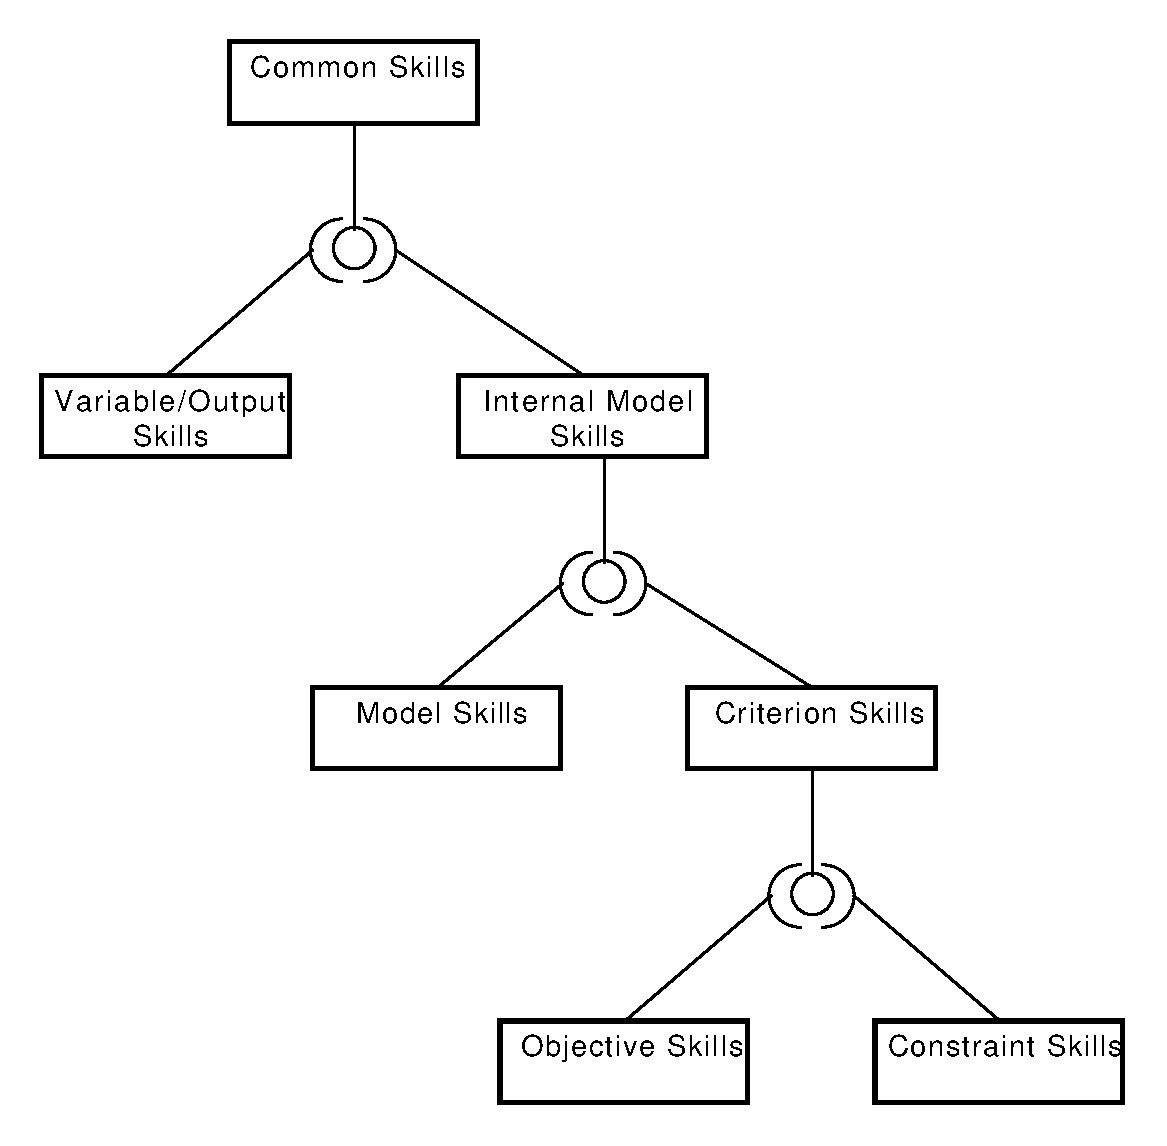
\includegraphics[width=\textwidth]{ID4CS_Speadl_skills}
			\caption{Skills components dependencies tree.}\label{skills:graph}
	\end{subfigure}
	\begin{subfigure}[b]{0.49\textwidth}
			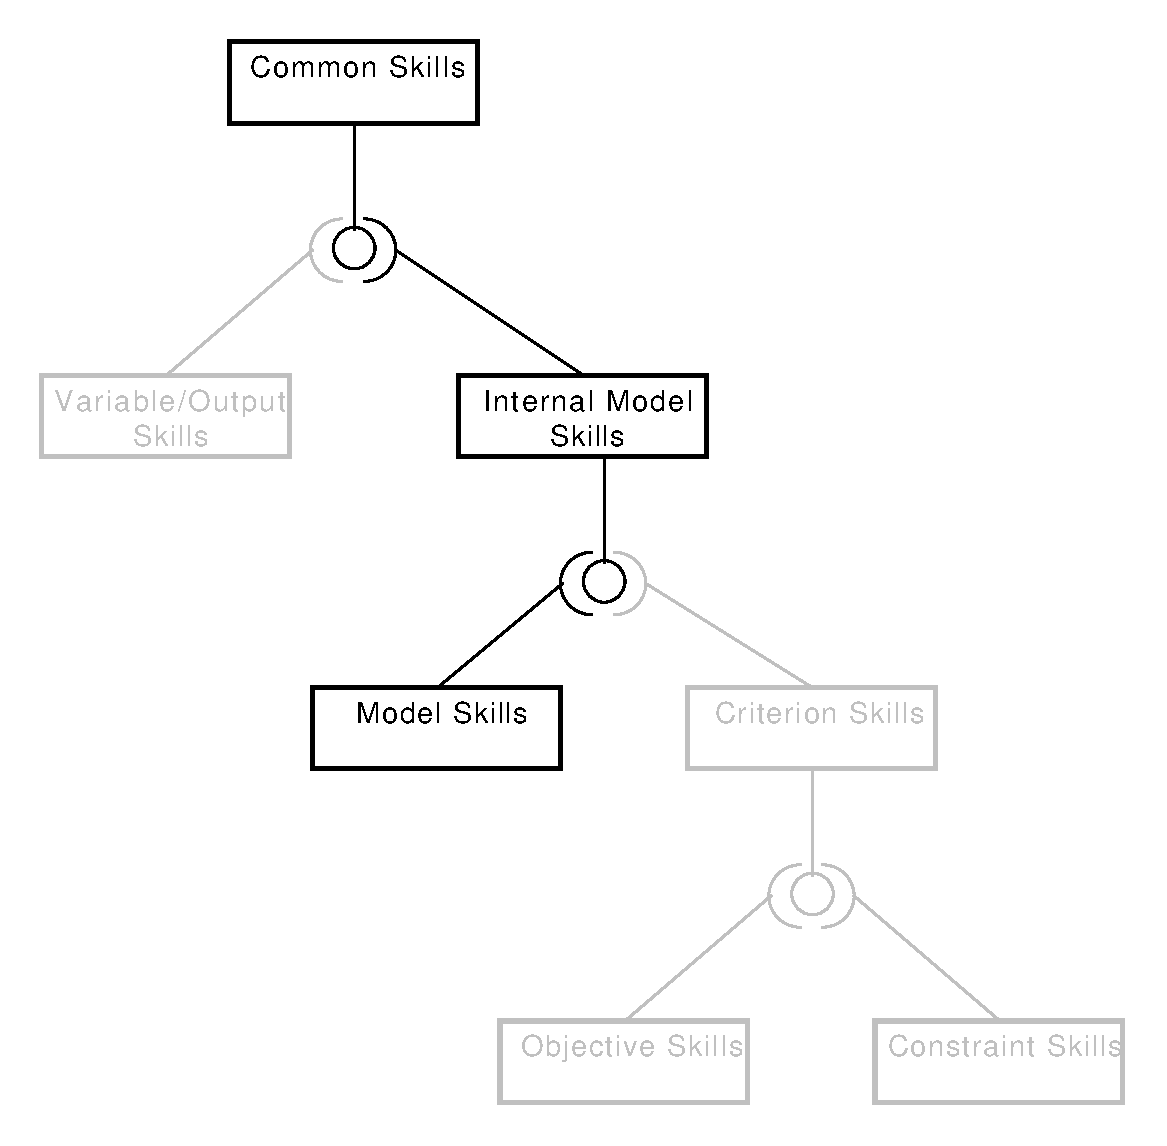
\includegraphics[width=\textwidth]{ID4CS_Speadl_skills_example}
			\caption{Model agent skills composition.}\label{skills:example}
	\end{subfigure}
\caption{\emph{Skills} component internals.}\label{skills}
\end{figure}

This tree-like structure of the skills components is not only a good way from engineering point of view a good way to factor implementation code, but is also efficient in regard of the functioning of NCS. As different NCS are shared by different agent types at different levels, this organization enables an efficient representation of [[correct ? => ]] which cooperative behavior is common to which agents. The NCS corresponding to the different components are shown in \figurename{} \ref{skills:NCS}

\begin{figure}
\centering
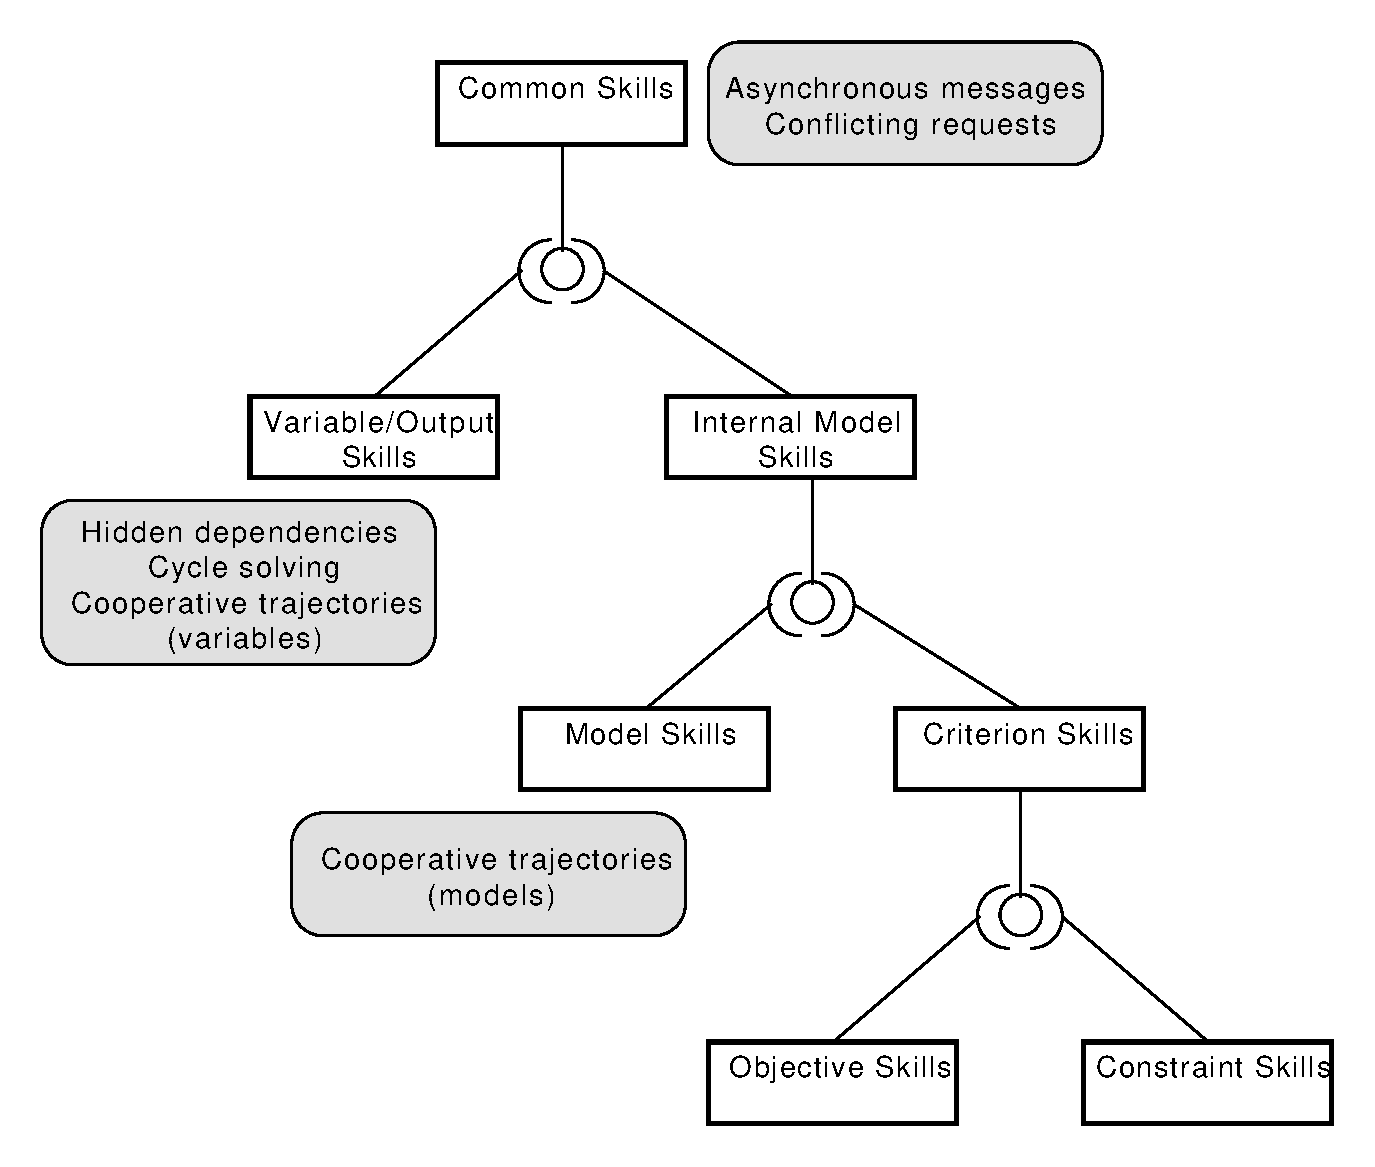
\includegraphics[width=\textwidth]{ID4CS_Speadl_skills_NCS}
\caption{Skills components dependencies tree with corresponding NCS.}\label{skills:NCS}
\end{figure}

\subsection{Communication}

The \emph{communication} view (\figurename{} \ref{Arch-comm}) presents the components related to the communication capabilities of the agent. 

\begin{figure}
\centering
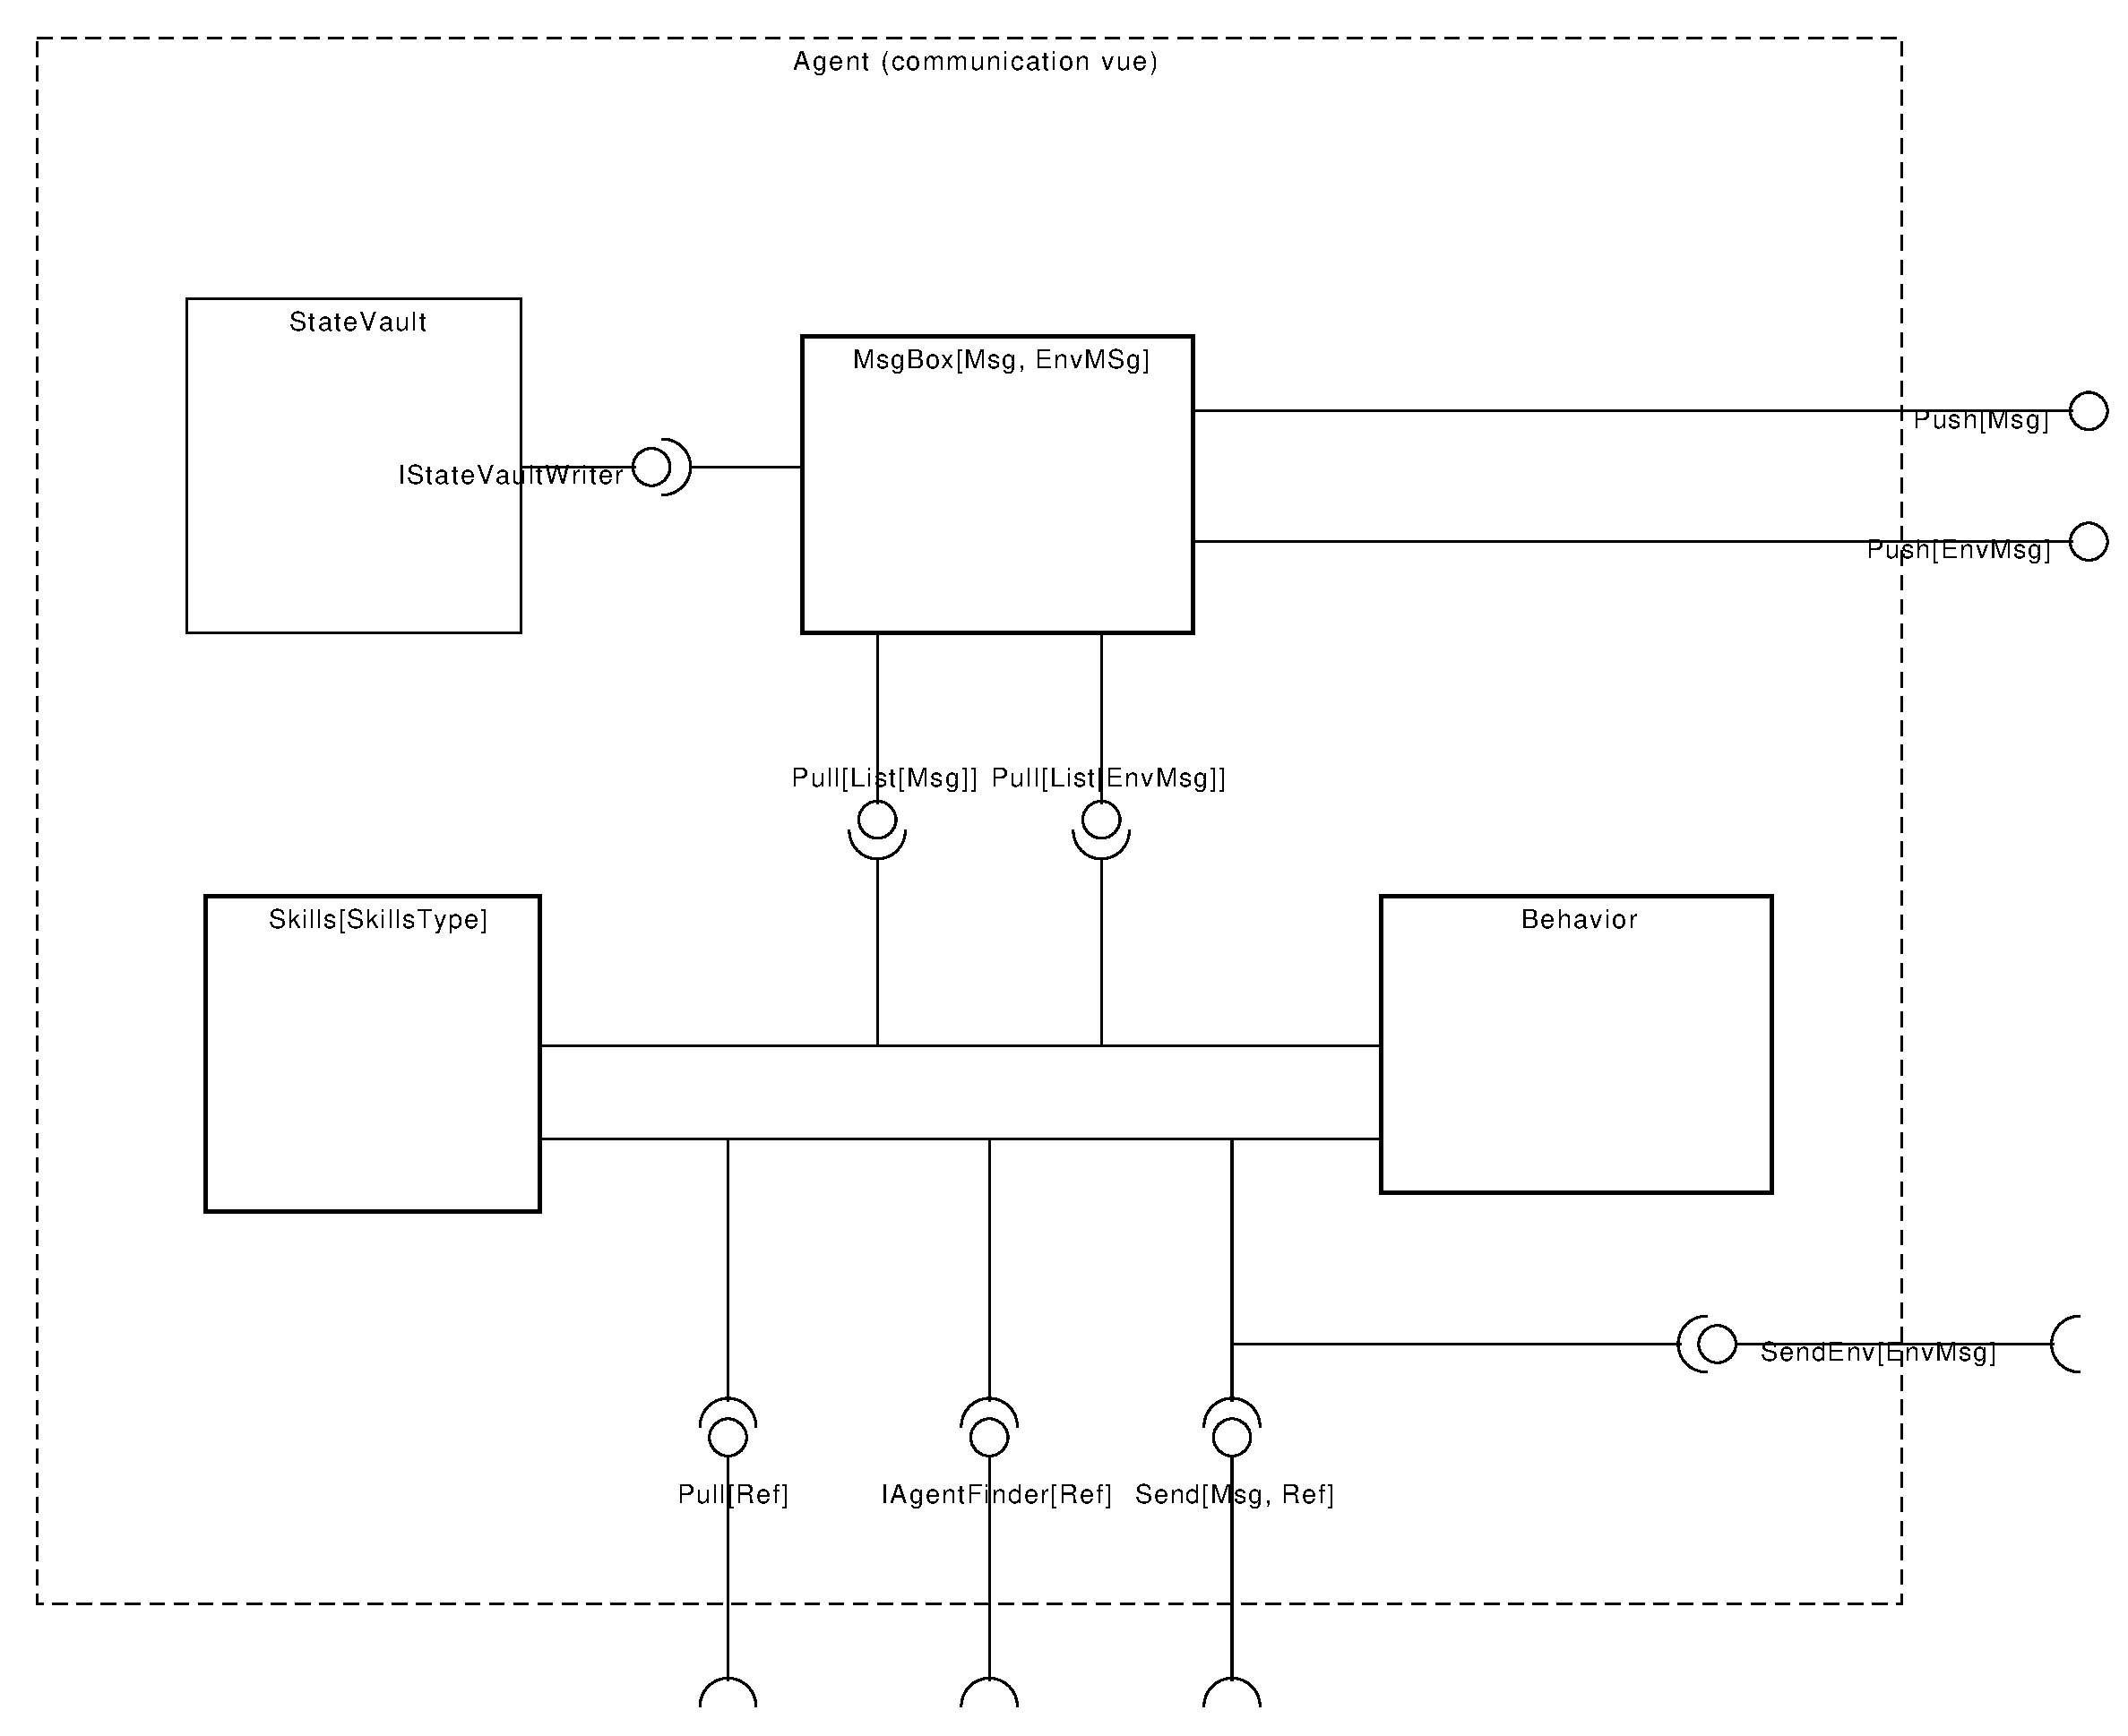
\includegraphics[width=\textwidth]{ID4CS_Speadl_comm}
\caption{Agent Architecture --- Communication view.}
\label{Arch-comm}
\end{figure}

This view contains the \emph{Message Box} component, which contains the messages sent to the agent. The \emph{Message Box} stores the messages into the \emph{State Vault} and provides a direct access to the \emph{Skills} and {Behavior} components.

This figure presents several ports which need to be provided from the environment to the agent. The environment must give an unique \emph{Reference} to the agent, which will be used by the other agents to communicate with it. The environment must also provides some ports to communicate with the other agents and outside of the system.

\subsection{Monitoring}

The \emph{monitoring} view (\figurename{} \ref{Arch-monitor}) presents the components related to the monitoring of the agent. It is used to observe the agents states and their modifications.

The new component introduced in this view is the \emph{Monitor}. The \emph{Monitor} provides two ports to the environment. The first port is used for external monitoring interfaces to subscribe to be informed of changes in the state of the agent. The second is used to provide informations concerning changes of a specific part of the agent. Thus, an external monitoring interface can subscribe in order to be notified when the state of the agent changed using the first port, and then use the second port to access to the specific informations it wants to monitor.

In order to provide its capabilities, the monitor component needs to be informed by the \emph{Behavior} component before and after each step, to read and compare the monitored informations into the \emph{State Vault}.

\begin{figure}
\centering
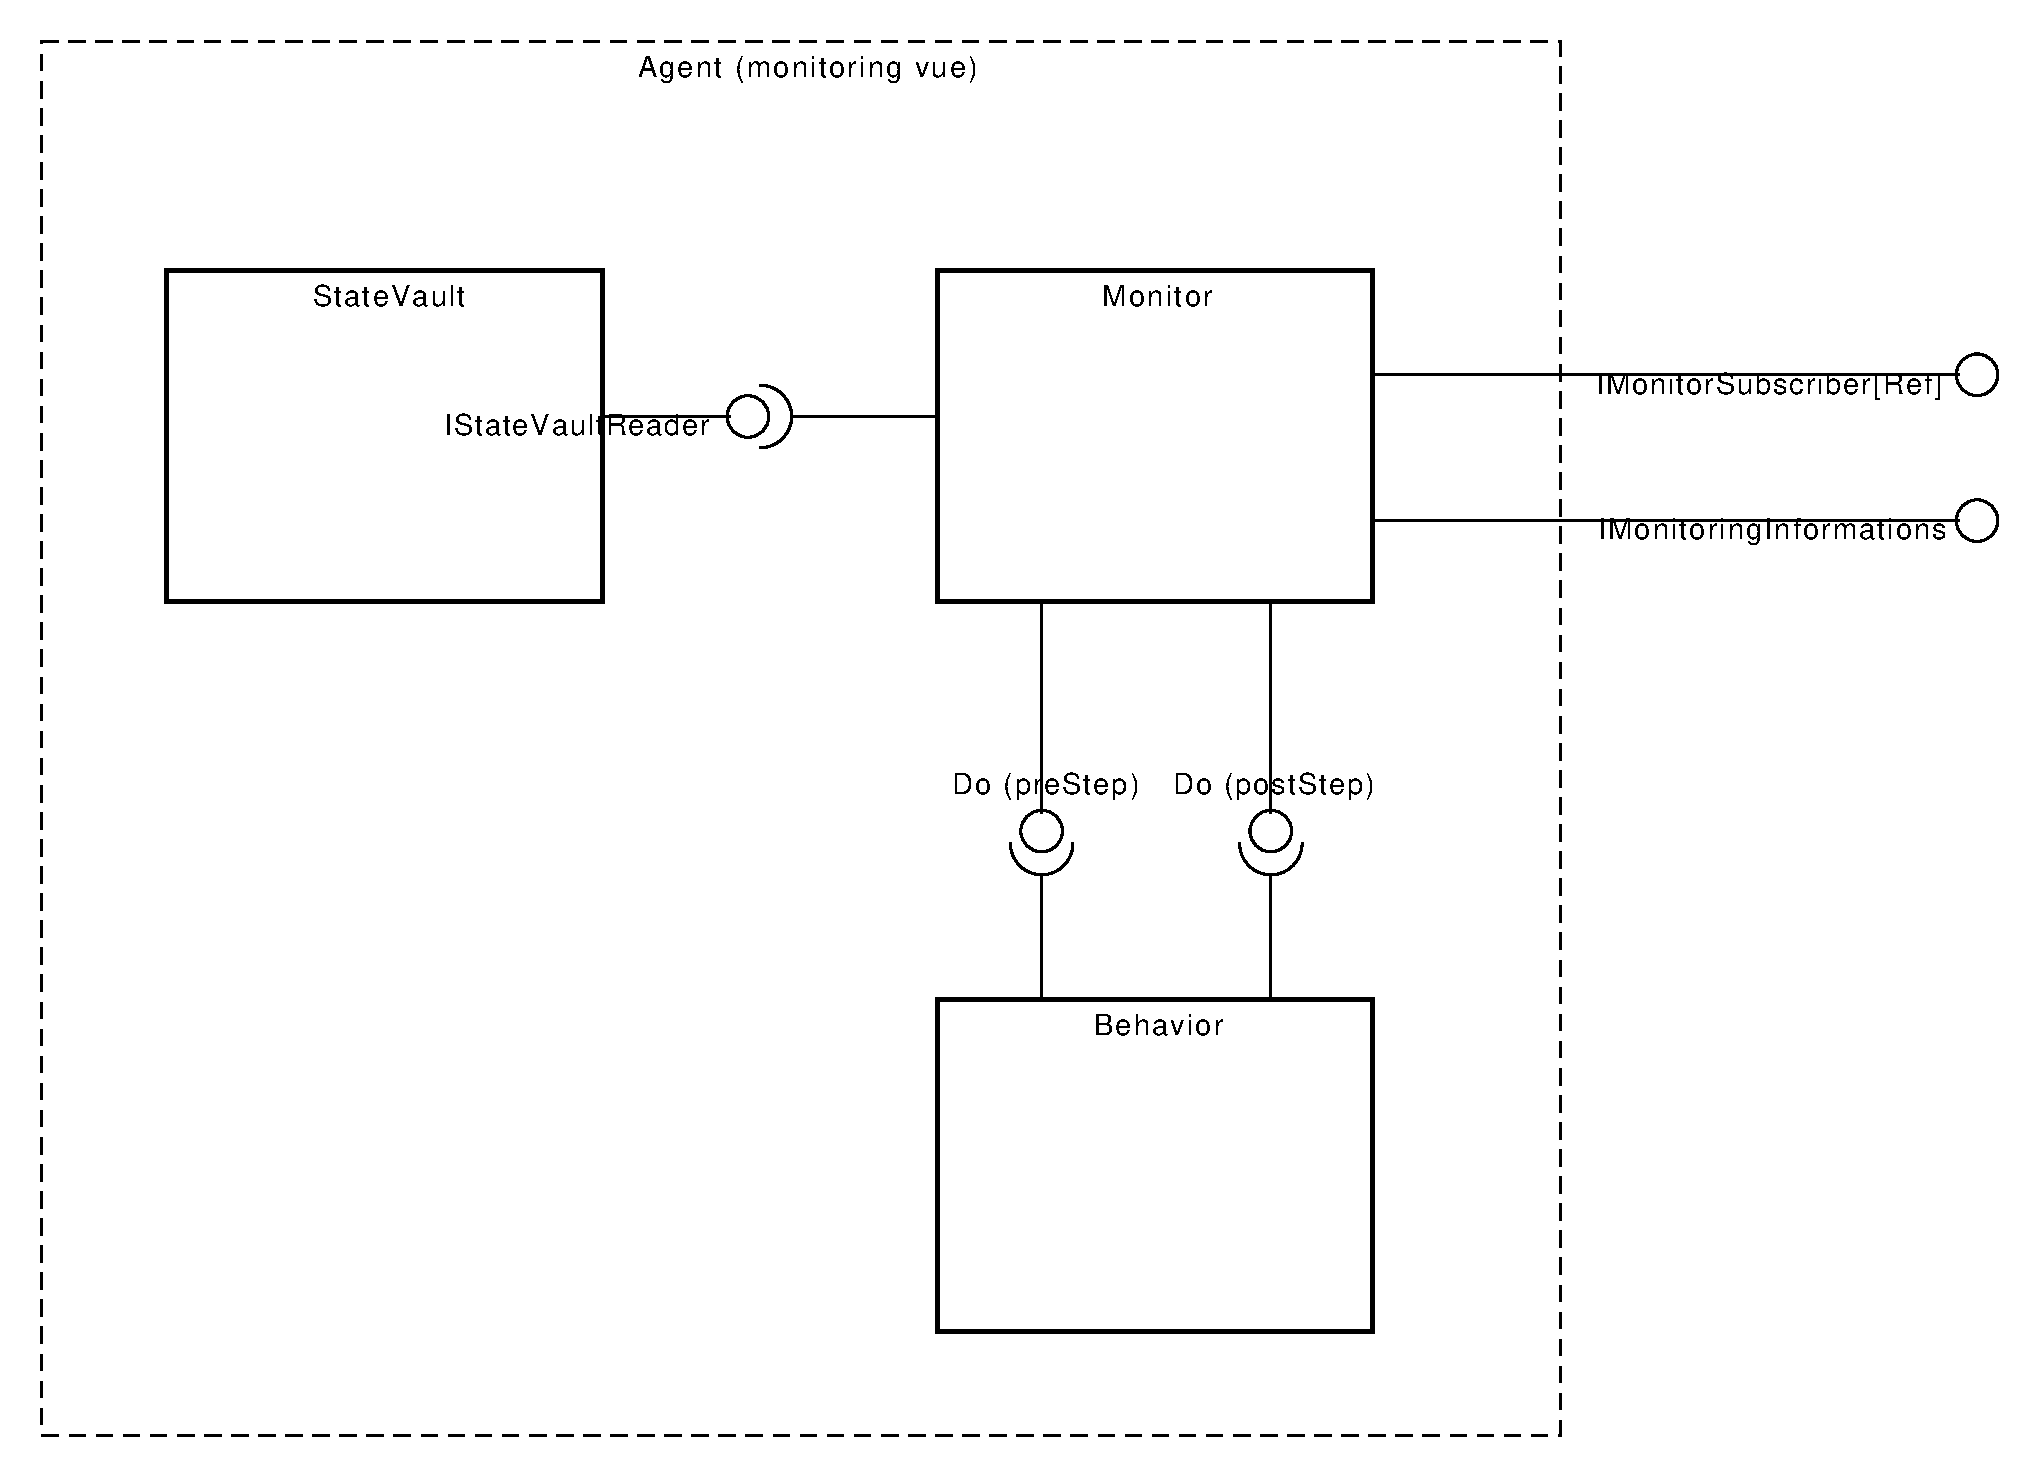
\includegraphics[width=\textwidth]{ID4CS_Speadl_monitoring}
\caption{Agent Architecture --- Monitoring view.}
\label{Arch-monitor}
\end{figure}

\section{MAY MAS Architecture}

The MAY framework does not only allow to design the architecture of the agents, but can also be used to design the whole architecture of the MAS. This MAS architecture defines how the agents can interact among themselves and with their environment. Concerning our prototype, this architecture first provides support for the messages passing among the agents. The architecture of the system, which is explained below, is shown on \figurename{} \ref{Arch-MAS}.

\begin{figure}
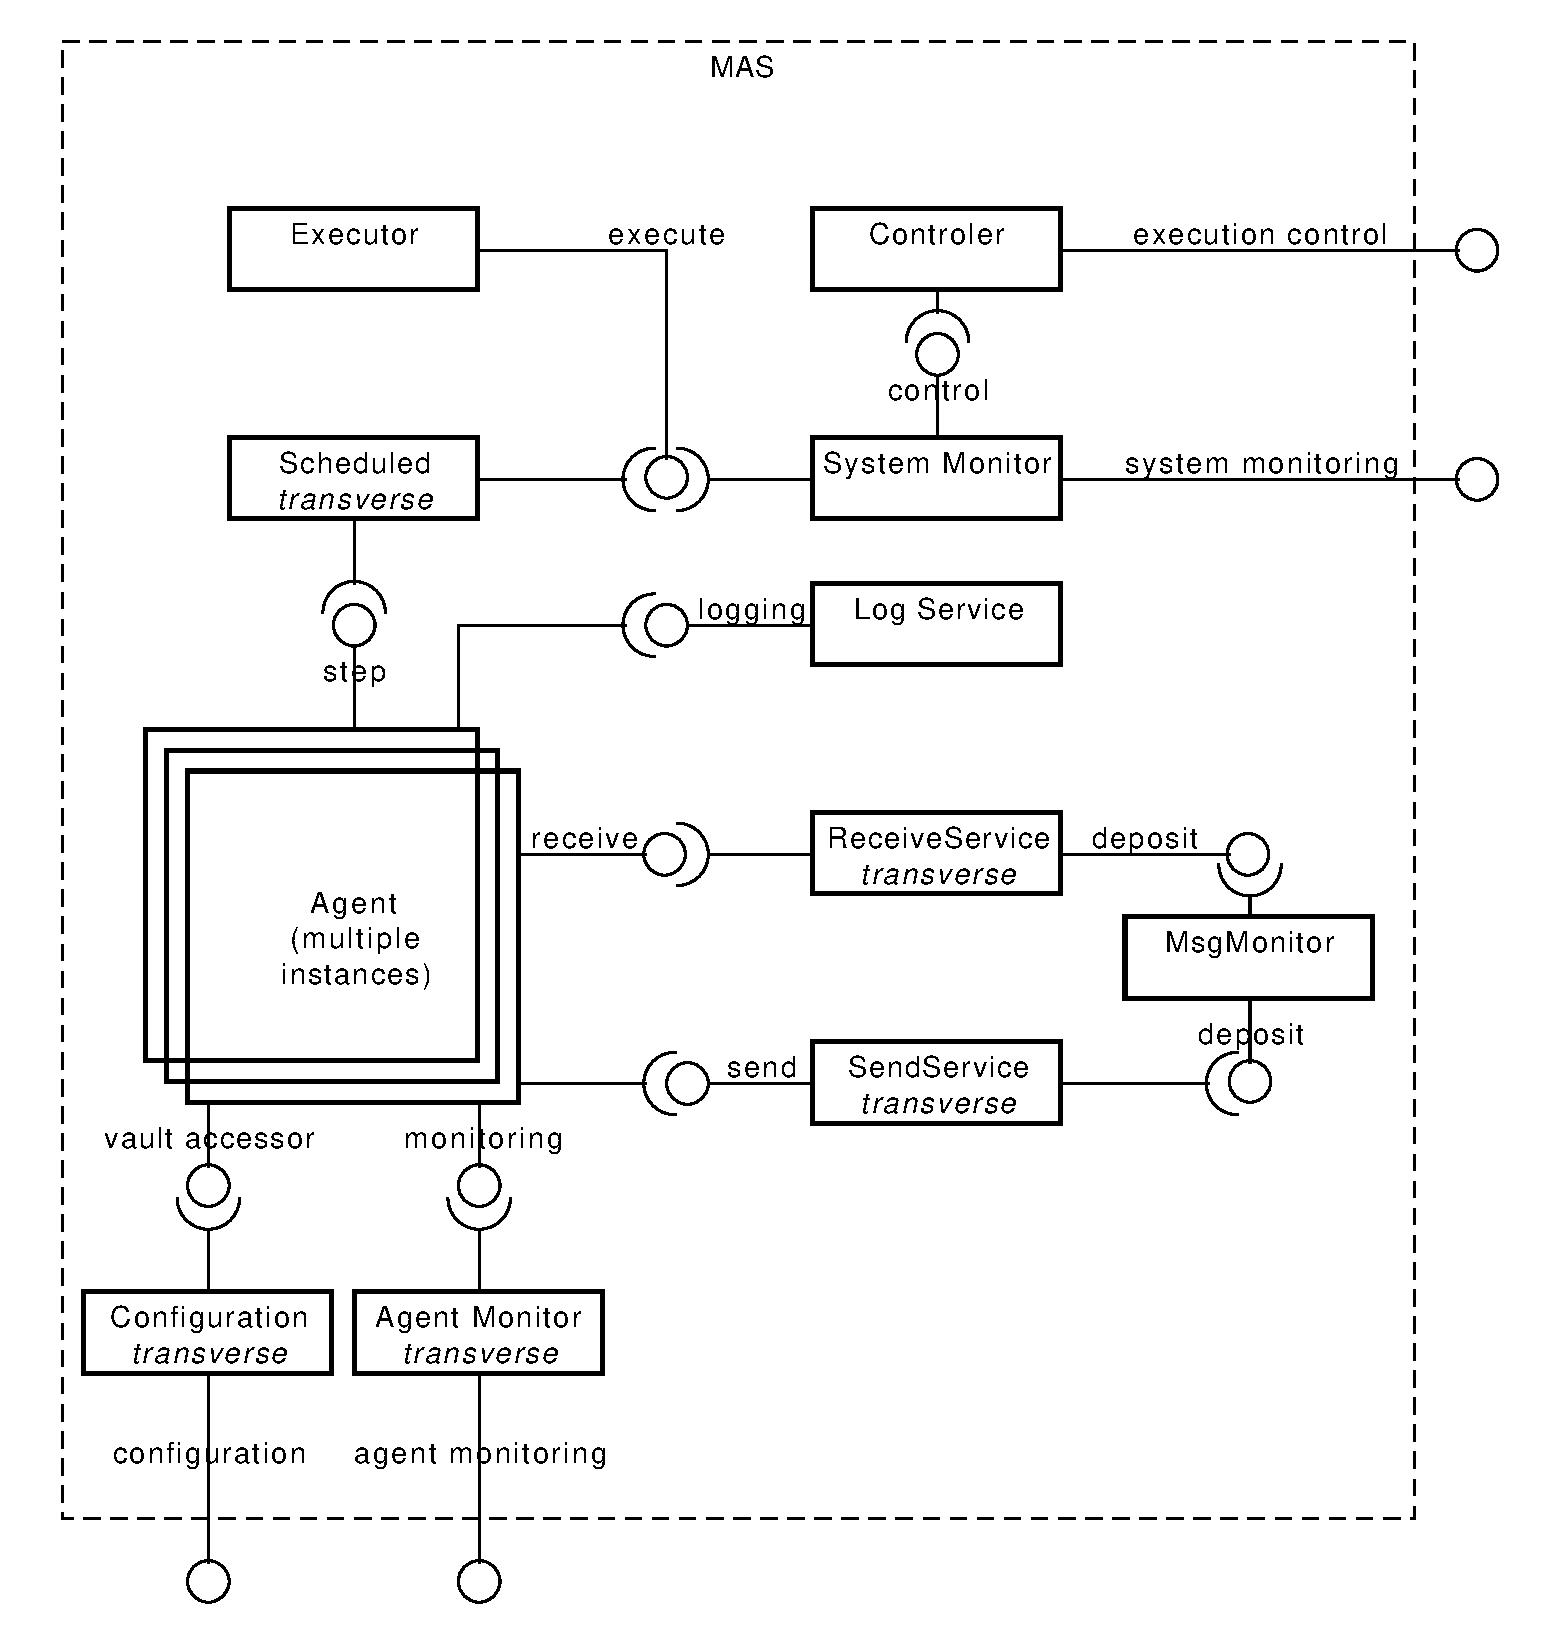
\includegraphics[width=\textwidth]{ID4CS_Speadl_system}
\caption{MAS Architecture.}\label{Arch-MAS}
\end{figure}

In order to support the integration of multiple agent instances into the global system architecture, MAY provides the concept of \emph{transverse}. A transverse is a special kind of component which makes the liaison between a component on one side and multiple instances of a component on the other. The main use of transverses is to connect all agents instances to the others components of the system.

The components \emph{SendService} and \emph{ReceiveService} are MAY components used to exchange messages between the agents. While they are usually directly connected together, we inserted between them a \emph{MsgMonitor} component, which allows us to monitor the messages transmissions. The agents also have the capability to create log messages to be written into log files using the \emph{Log Service} component.

Some interfaces for configuring and monitoring the agents are exposed to the outside of the MAS through the \emph{Configuration} and \emph{Agent Monitor} transverses. The \emph{Agent Monitor} component exposes some representative information on the agents, while the \emph{Configuration} component offers a direct access to the agent state vault, allowing to examine the raw data as well as offering ways to the user to interact with the agents (changing values, constraints thresholds \emph{etc.}).

A more complex monitoring interface is provided by the \emph{System Monitor}. This component not only allows for advanced monitoring functionalities (like subscribing to changes notifications), but also handles the execution of the system though the \emph{Executor} component. The \emph{Executor} handles the low-level execution concerns, like creating threads and executing tasks, and is in charge of executing the code of the agents through the \emph{Scheduled} component. A very similar configuration (not presented on the diagram) allows the agents to exchange messages with the outside of the system. The \emph{System Monitor} is linked to a \emph{Controler} component, which is in charge of exposing a convenient execution control interface for the user or for an external program.

\section{Integration into the Prototype}

This implementation of the MAS was part of a collective development effort to provide a functional prototype. The goal of this prototype is to be a end-user aimed tool of the possibilities offered by agent-based continuous optimization.

The development of the prototype was carried mainly by three partners[[cite them?]], each in charge of a different aspect.

The prototype can be divided in three parts: The Graphical User Interface (GUI), the core module (CORE) and the Multi-Agent System (MAS). The CORE provides a common representation of the manipulated data and is in charge of maintaining consistency between the GUI and the MAS.

These three modules communicate using the OSGi framework\footnote{\url{http://www.osgi.org}}.

\subsection{MAS}

The MAS implementation is the main contribution of this thesis and was already presented in the previous parts. The only additional work was to encapsulate the implementation into an OSGi bundle which exposes the functionalities corresponding to the external services exposed by the MAS architecture and presented in the previous section.

\subsection{CORE}

The CORE module is responsible of maintaining consistency of the manipulated data. It serves as a middle-man between the MAS and the GUI. It also makes possible to enable data persistence by providing a serialization/deserialization service.

\subsection{GUI}

The GUI was build using the Eclipse Rich Client Platform (RCP)\footnote{\url{http://wiki.eclipse.org/index.php/Rich_Client_Platform}}. RCP allows to compose graphical interface components into a user interface. It was used to propose graphical tool inspired by existing development environments, providing the user with the possibility to define workspaces in which it can define problem elements which can then be used to define optimization problems.

\bigskip

By combining these three modules, we obtained a prototype which can be used to create optimization problems. To create a problem, the user can either provide a textual definition or use the graphical tools. In the last case, the user defines different reusable components (variables, models \emph{etc.}). He is then able to drag-and-drop them from an element palette on a graph canvas and to draw links between the different elements, effectively creating the problem using our NDMO graph representation. Either way, the problem is automatically translated in an instance of the MAS, which can be controlled by the user during the optimization process. A screenshot of our prototype, showing the graph canvas on which the graph of a problem is currently being created, is shown on \figurename{} \ref{tool}.

\begin{figure}
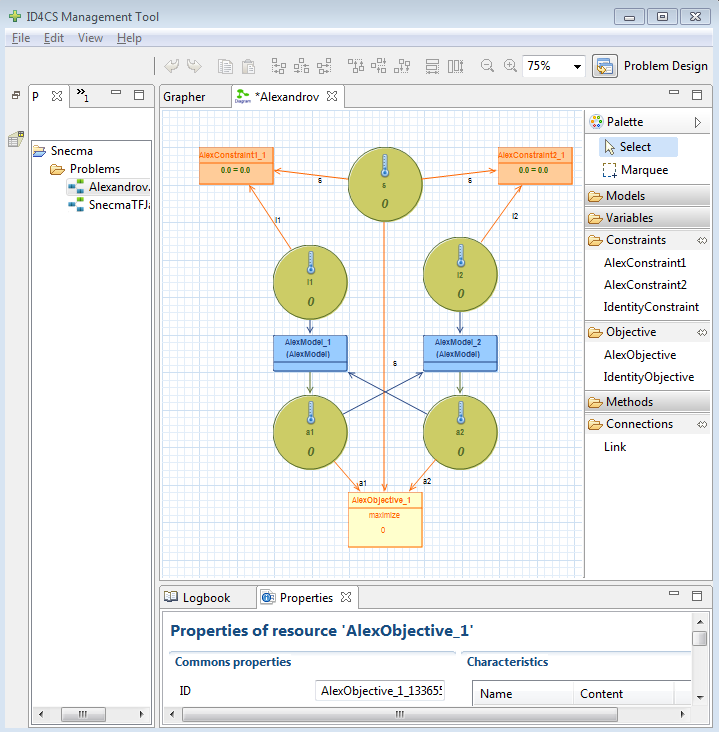
\includegraphics[width=\textwidth]{tool}
\caption{User Interface of our prototype (problem canvas view).}\label{tool}
\end{figure}

\chapter{Collective Problem Solving Patterns}\label{CPSP}

We have seen in the previous chapter how the ADELFE methodology was used for the design of AMAS, from the general requirements to the implementation of the agents. However a current limitation of ADELFE (shared with most of the existing comparable methods) comes from the fact that it aims to be applicable for designing MAS intended for diverse application fields (problem solving, simulation, \emph{etc.}). This desire to be usable for a large spectrum of applications has the drawback that the recommendations and guidelines of ADELFE are often quite abstract and high-level. This makes the task of actually designing an AMAS for a precise application domain difficult for non multi-agent expert.\\
This limitation has already been observed in previous works, and has given birth to an ongoing effort in the SMAC team to provide a modular toolkit named \emph{AMAS for Optimization} (AMAS4Opt), with the goal to supplement ADELFE and assist AMAS designers when designing AMAS for problem solving. In the same way that some contributions have already been proposed in the context of combinatorial optimization (see \cite{Ka2011.6}), we will now see how we can propose to enrich the toolkit in the context of continuous optimization.

In this chapter, we take a step back from the MAS we described in the previous parts[[]] and see how our contribution can be made more general, not only to the benefit of the scientific community, but also for engineers by enriching AMAS4Opt.\\
Continuous optimization was a mostly unexplored application domain in regard to multi-agents based algorithms. By taking the (somewhat ambitious) task to propose a MAS which would be applicable for this domain as a whole, some of the patterns identified and some of the mechanisms we proposed can be used in a more general context than our system.

As continuous optimization is in itself an abstract mathematical field, we too had to abstract ourselves from concrete applications. We did not have the possibility to reduce the set of possible configurations and thus we had the occasion to encounter a variety of problems which have been mostly ignored before. Indeed, the graph representations of numerical optimization problems are quite diverse, and can present some topological properties not present in existing MAS formalisms.

In the description of our system, we presented a set of NCS [[use acronym ?]], and the specifics mechanisms we introduced to handle them. We believe that these NCS are only the instantiation of more general problematic topologies, which we dub \emph{Collective Problem Solving Patterns} (CPSP). The patterns are not restricted to continuous optimization and can potentially be encountered in all sorts of application domains.

Architecture and software development has greatly benefited from the identification of common design patterns. In the same way, we believe that the identification of these patterns as such, as well as of specific solutions to handle them, could lead to a great improvement for the design of agent-based systems as a whole.

Consequently, we will present in this part how the NCS we identified during the design of our system can be abstracted in the broader form of CPSP.


\section{Introduction - Collective Problem Solving Patterns are not Design Patterns}

[[EXPLAIN THE DIFFERENCE WITH EXISTING AGENT PATTERNS]]

Before describing the CPSP in themselves, we must explain how these patterns differ from the existing design patterns for MAS.

There is already an existing (if limited) corpus of design patterns for MAS. These patterns have usually in scope either the design of the organizational structure of system or the design of the behavior architecture of the agents. They concern the \emph{design} of the system itself regarding the target application domain. Consequently they are relevant for the design of the \emph{organization of the system}, according to the application domain.
What we propose here is a different sort of patterns, which concerns the \emph{behavior of the agent}, according to an existing organization. Design Patterns concern the structural aspects of the system, while Collective Problem Solving Patterns concerns its functional aspects.

In this regard, CPSP are less generic than Design Patterns. Indeed the latter can be applied to the whole range of MAS, while the former only concerns MAS designed for problem solving (excluding, for example, MAS for simulation).\\
These two kinds of patterns should be seen as complementary.  First the designer could use design pattern to design the structure of the MAS according to the needs of the application domain. Then he could use CPSP to identify and solve specific problems resulting from such modeling and from the application domain itself.

As we want a description of our patterns which is domain-free, we cannot re-use the NDMO modeling we introduced in \ref{modeling}, which is dedicated to the domain of continuous optimization. Consequently, we will now introduce a higher-level formalism, which concentrates on the relations between the agents of the system. To keep this formalism short and simple, we will make some assumptions about the functioning of the system.

We consider systems composed of autonomous agents and resources. An agent may require that some resources be in a specific state, to accomplish its local goal. We will also suppose that a resource is controlled by one agent and one agent only. We believe that this simplifying assumption does not impede on the generality of the formalism (since a system where two agents share the control of a resource can be viewed as equivalent to a system where both agents send requests to a third one solely in charge of it). At last we will suppose that agents interact among themselves by direct message passing.

\section{Description of a Problem Solving Pattern}

\subsection{Agent Roles}\label{CPSP_roles}

The work of \cite{Ka2011.6} proposed a modeling of agent roles related to the application domain of constrained combinatorial optimization composed of the \emph{Service} and \emph{Constrained} roles. While this taxonomy was adequate for the description of this application domain, it is not general enough for our goal. Since we want the CPSP to be abstracted from any application domain, it is also necessary for the agent role modeling to be abstracted. Concerning the patterns we present in this article, we identified three different types of agent \emph{roles}: Provider, Solicitor and Transformer. There is an obvious matching between \semph{service} and \emph{provider} roles, and between \emph{constrainted} and \emph{solicitor} roles, indicating that these two modelings are essentially representing similar things at different abstraction levels.

The \emph{Provider} role represents the fact that the agent is in charge of a given resource, which can be of use to others agents in the system. The agent is responsible for choosing the state of the resource or giving access to it based on solicitations of the others agents.

The \emph{Solicitor} role represents the fact that the agent requires that some resource(s), which it does not control, be in a specific state, in order to accomplish its goal. Consequently, the agent needs to solicit the agent(s) controlling the relevant resource(s).

The \emph{Transformer} role is a combination of the Provider and Solicitor roles. The transformer agent controls a resource but the state of the resource is dependent of some other resources not controlled by the agent. While this role can be represented by assigning both Provider and Solicitor roles to the agent, we found this role common enough to be worth a specific representation. As we will see, transformer agents sometimes play a specific role in some CPSP, as they can be a source of delay or obfuscation of information.

On \figurename{} \ref{cpsp_class_diag} is shown the very simple class diagram representing the relationships between these three roles.

\begin{figure}
\centering
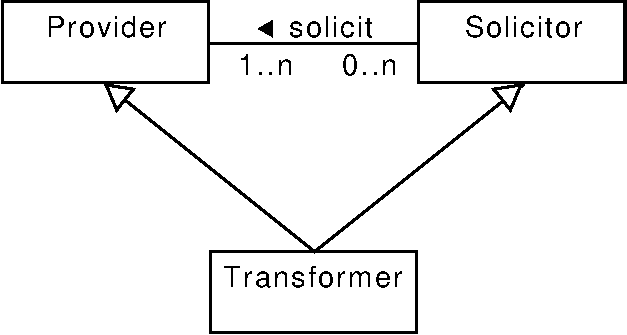
\includegraphics[width=0.5\textwidth]{cpsp_class_diag-crop}
\caption{class diagram of the Provider-Solicitor modeling.}
\label{cpsp_class_diag}
\end{figure}

It is important to understand that an agent is not limited to one role only. For a given system an agent can, depending on the context, assume any combination of these roles. Thus an agent can both solicit others agents regarding a resource, while being  at the same time a provider of another resource.
In this regard, an agent can even be a producer and solicitor of the same resource. For example the agent is in charge of a specific resource, but also benefit from it. In this case the agent can possibly be in conflict with others agents regarding the state of the resource, and decides (as a producer) to go against its own interest (as a solicitor) in order to help another agent deemed more important.
Obviously, in most implementations, the different roles of the agent would not be as much segregated, and the agent would not strictly communicate with itself using message passing. This distinction should not be a problem in practice (this kind of configuration can however trigger other CPSP, see for example \ref{NCS_async}).

For example, in the case of our system, the different agent types have relatively defined and fixed roles. A design variable agent linked with at least one other agent has a \emph{provider} role. Constraint and objectives agents are \emph{solicitors}. Models agents have a \emph{transformer} role, as for output agents which are in input of at least one model or criterion agents.\\
The only agents which do not have roles corresponding to this taxonomy are the variable and output agents which are not used as input by any other agent. And indeed in our system these agents would have a basically non-existent role. Of course the user can still manually intervene to change the topology of the problem, changing at the same time the roles of these agents.

\subsection{Pattern Description}

For each CPSP, we provide a short description. This description will obviously be quite similar to the description of the NCS[[s]] in \ref{NCS_pres}, as they correspond to the same pattern, only from different abstraction levels.

As we already presented the details of the different mechanisms in section \ref{NCS_pres}, we will not detail them again in this part. Moreover, the CPSP aim to be general patterns applicable to multiple domains, consequently it is not possible to fully specify them. A part of the instantiation work  must still be done by the designer. However we discuss some conditions which are necessary in order to instantiate to the domain the handling mechanisms we proposed.

For each CPSP, we also provide a synthetic \enquote{blueprint} which is composed of two parts:
\begin{compactenum}
\item a representative agent configuration of the CPSP (using the agent roles introduced in section \ref{CPSP_roles}) 
\item a summary of the mechanisms involved in the solving of the CPSP.
\end{compactenum}
These blueprints are based on the template shown on \figurename{} \ref{blueprint_template}.

\begin{figure}
\centering
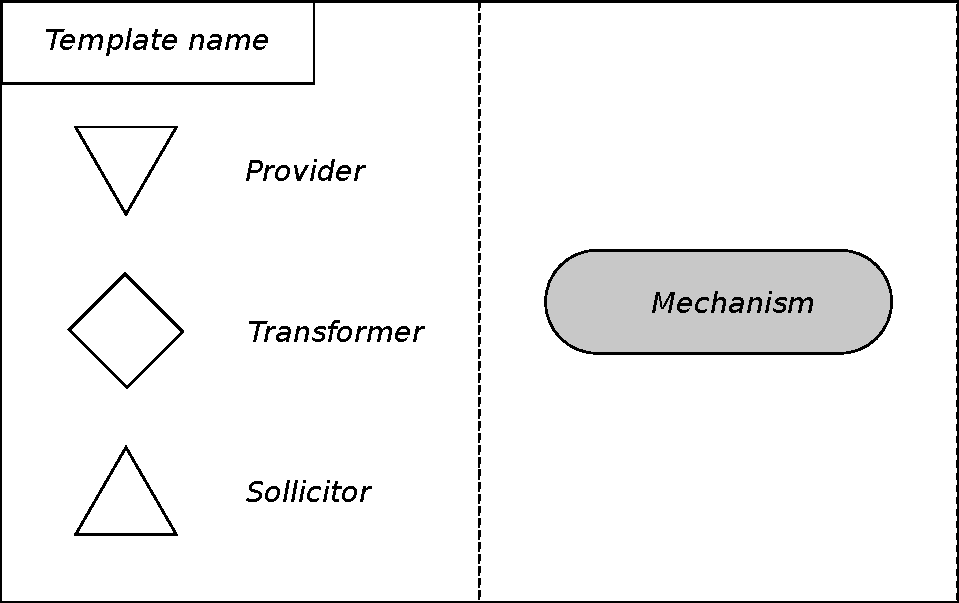
\includegraphics[width=0.6\textwidth]{blueprint_template}
\caption{Template on CPSP blueprints.}\label{blueprint_template}
\end{figure}

\section{Identified Collective Problem Solving Patterns}

In this section, we present the CPSP we identified from the NCS we encountered during the design of our MAS.

\subsection{Conflicting Requests}

In this situation a provider agent is requested to do different conflicting actions from several solicitors agents. This CPSP is probably the simplest one and was already identified as a recurring situation in previous works on AMAS, as it is the direct instantiation of the \emph{Conflict} NCS category (as presented in section \ref{amas_theory}).

The blueprint of this CPSP is shown on \figurename{} \ref{blueprint_conflicts}.

\begin{figure}
\centering
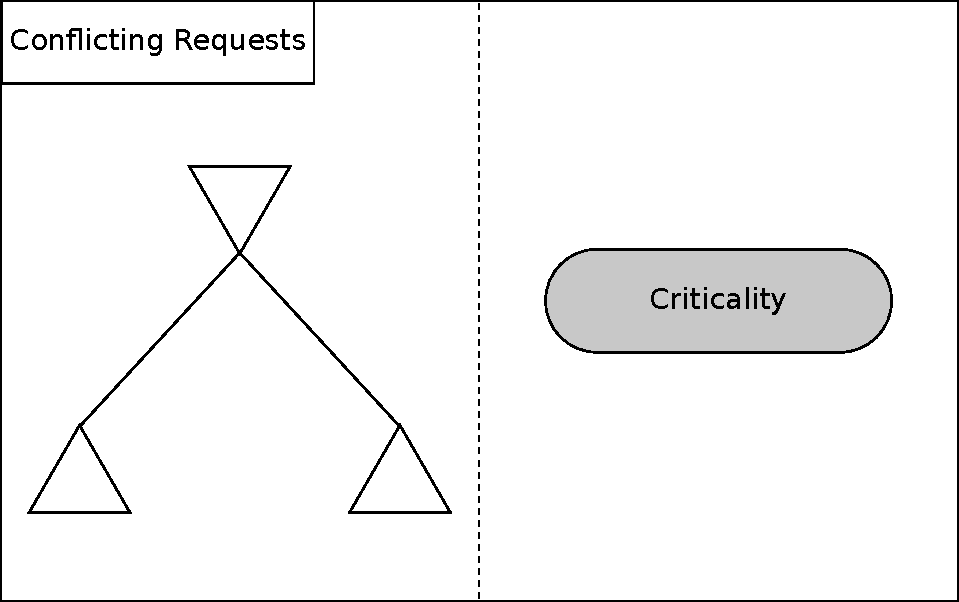
\includegraphics[width=0.6\textwidth]{blueprint_conflicts}
\caption{Conflicting Requests blueprint.}\label{blueprint_conflicts}
\end{figure}

In order to apply the blueprint, the designer must be able to define a common and comparable measure of the \enquote{dissatisfaction} state of the solicitors. This \emph{criticality} must be transmitted with the requests made by the solicitor agent.

The use of a criticality measure as way to discriminate between the different requests is a \enquote{tried-and-true} technique which has been applied to multiple AMAS applications [[cite some]].\\
As a remark, a measure of dissatisfaction presents an advantage over a measure of satisfaction in the fact that it is often possible to estimate the state of maximal satisfaction of the agent (every requirement is perfectly satisfied), but not always possible to do so for the maximal dissatisfaction. Consequently a measure of satisfaction would have a upper bound but no lower bound, while a measure of dissatisfaction has a lower bound and no upper bound. This latter is easier to manipulate and reason with as it can be easily be represented by an unbounded positive value.

\subsection{Cooperative Trajectories}

[[TODO]]

\begin{figure}
\centering
	\begin{subfigure}{0.49\textwidth}
		\centering
		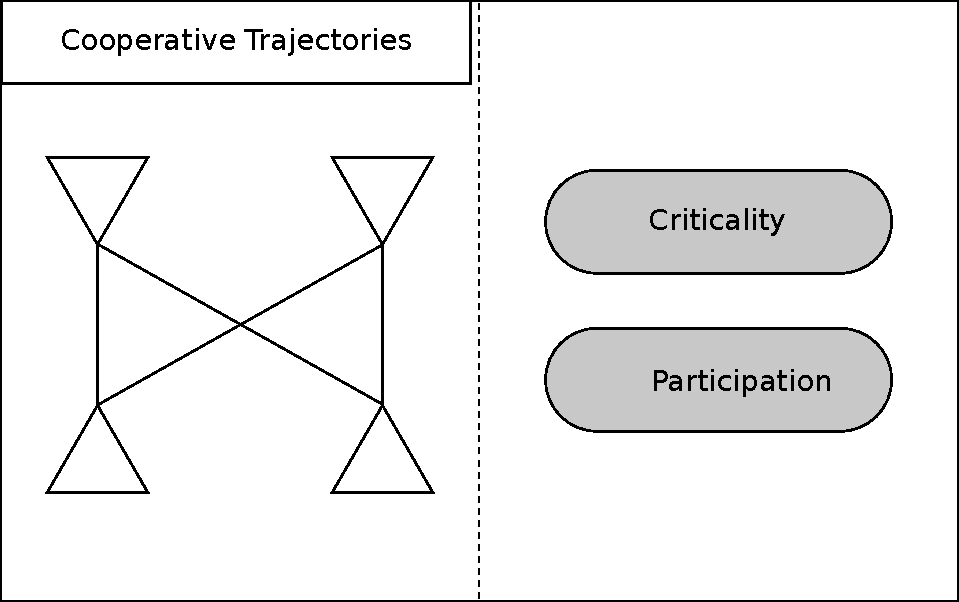
\includegraphics[width=\textwidth]{blueprint_coop_traj_var.pdf}
		\caption{Direct.}
	\end{subfigure}
	\begin{subfigure}{0.49\textwidth}
		\centering
		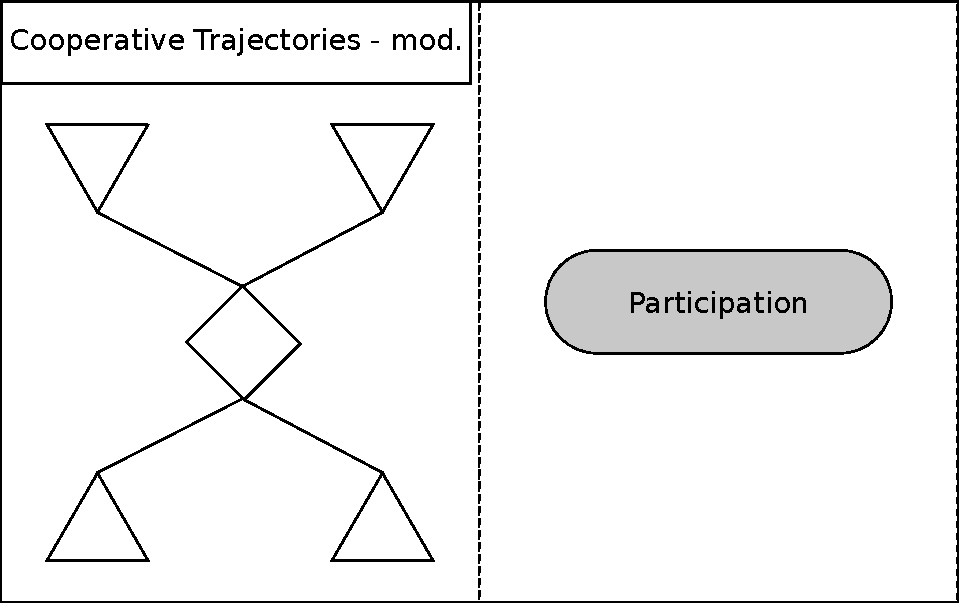
\includegraphics[width=\textwidth]{blueprint_coop_traj_model.pdf}
		\caption{With a Transformer agent.}
	\end{subfigure}
\caption{Cooperative Trajectories.}\label{blueprint_coop_traj}
\end{figure}

[[REALLY DO TWO FIGURES ? ONE IS BASICALLY A VARIANT OF THE OTHER]]

\subsection{Cycle Solving}

[[TODO]]

\begin{figure}
\centering
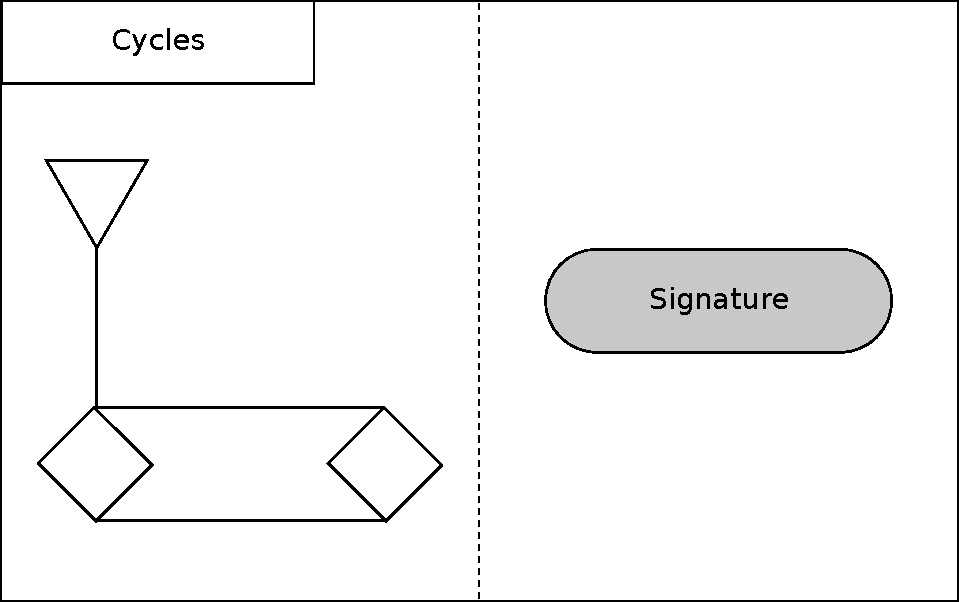
\includegraphics[width=0.6\textwidth]{blueprint_cycles}
\caption{Cycle Solving blueprint.}\label{blueprint_cycles}
\end{figure}

\subsection{Hidden Dependencies}

The hidden Dependency CPSP arises when a solicitor agent assumes the agents to which it sends requests are independent providers, while one of them is in fact dependent of the other (transformer role). This pattern leads to a suboptimal behavior when the solicitor agent sends requests which are contradictory for the \enquote{top-most} provider agent. The blueprint of this CPSP is shown on \figurename{} \ref{blueprint_hidden_dep}.

\begin{figure}
\centering
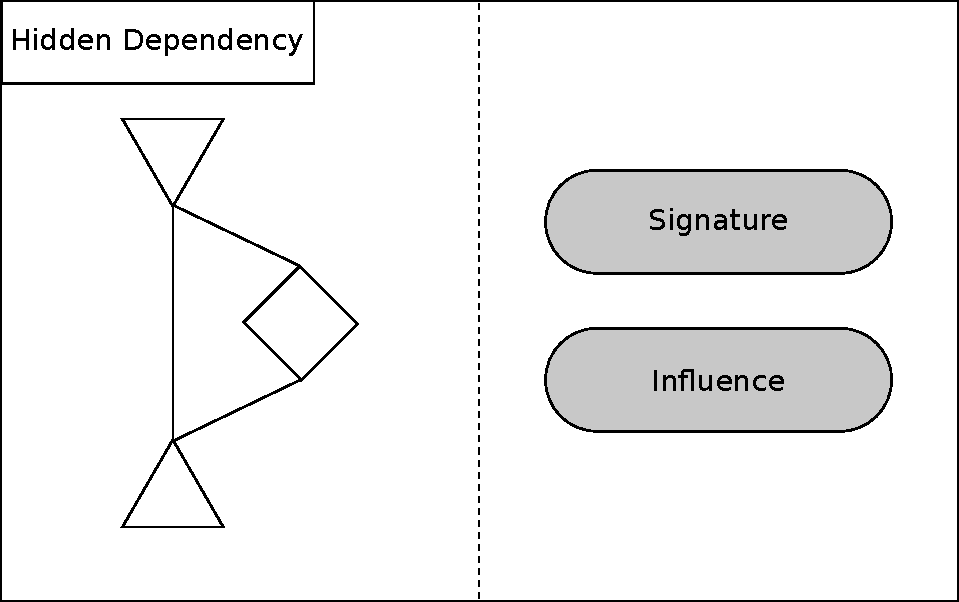
\includegraphics[width=0.6\textwidth]{blueprint_hidden_dep}
\caption{Hidden Dependencies blueprint.}\label{blueprint_hidden_dep}
\end{figure}

To apply this blueprint, the designer has to complement the messages exchanged by the agents with unique signatures containing an immutable \emph{origin}, which uniquely identify the agent that is the origin of the request. The designer must also be able to define an \emph{influence} measure to be transmitted with the request, that represent the impact of the recipient on the solicitor. These \emph{influences} measures must be comparable for a same origin.

\subsection{Asynchronous Requests}

This CPSP arises when a provider agent receives requests from multiple solicitor agents, but these requests arrive in a desynchronized manner. A possible suboptimal behavior can happen when the provider agent decides to satisfy a request from a solicitor, and receives afterward a more important request contradicting the first one. The blueprint of this CPSP is shown on \figurename{} \ref{blueprint_async}.

\begin{figure}
\centering
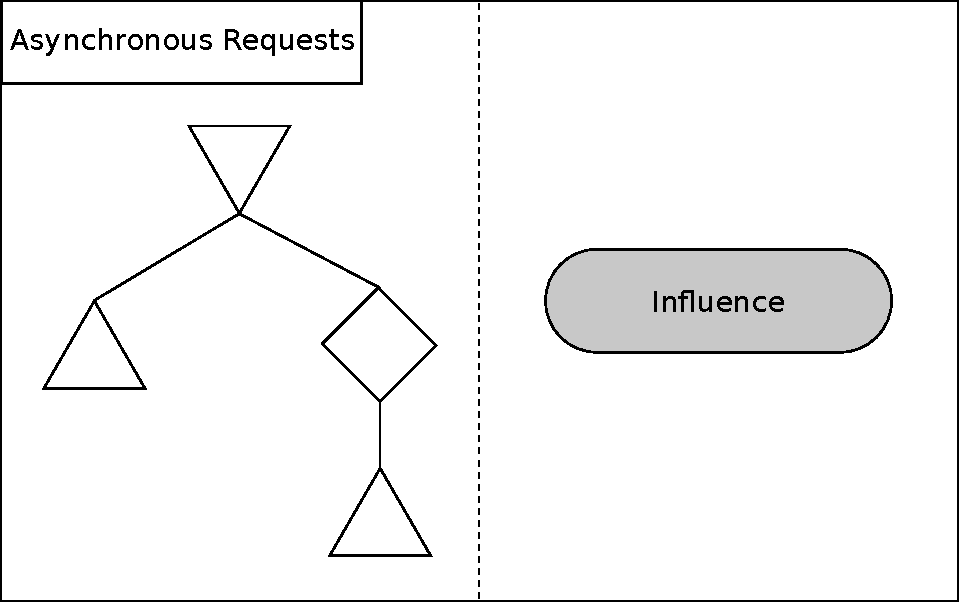
\includegraphics[width=0.6\textwidth]{blueprint_async}
\caption{Asynchronous Requests blueprint.}\label{blueprint_async}
\end{figure}

To apply this blueprint, the designer must be able to define an \emph{influence} measure for each solicitor agent to estimate, that represents the impact of the recipient on the solicitor. This \emph{influence} will allow the solicitor agent to determine when it received enough informations to make a sufficiently informed decision, without needing to wait for \emph{all} the answers to its requests.\\
Alternatively, if answer delay of the solicited agents is negligible, or if for any other reason it is deemed acceptable that a solicitor agent waits for all the answers before taking a decision, the mechanism can be adapted to avoid using \emph{influence} altogether.

\section{Conclusion on Collective Problem Solving Patterns}

We have seen previously that the main contribution of this thesis was the proposal of a novel agent-based algorithm for the solving of complex continuous optimization problem. In this chapter we present an addition contribution in the form of general Collective Problem Solving Patterns. These CPSP are the generalization of the different NCS we identified during the design of our MAS and have for goal to assist the designer of the system in the identification of potentials problems which may arise from the agents organization, as well as to propose some possible handling mechanisms to handle them.

We presented a general agent role modeling which is abstracted from any precise application domain. This modeling presents the \emph{Provider} and \emph{Solicitor} roles, and their extension by the \emph{Transformer} role.

Using this modeling, we presented some CPSP \emph{blueprints} which expose in a synthetic manner the base agent pattern and the mechanisms involved in the solving of the CPSP. We also presented some of the conditions required for the designer to be able to instantiate the solving mechanism for his system.

Our agent role modeling is an extension of the one in \cite{Ka2011.6}, in which a first abstraction work has been done to identify general agent roles for constrained optimization. This previous work led to the identification of the \emph{service}and  \emph{constrainted} roles. However this previous modeling was restricted the field of AMAS for constrained optimization. In this regard it was not adequate for the description of the CPSP . Moreover, by explicitly introducing the \emph{transformer} role in our Provider-Solicitor modeling, we are able to express more clearly some of the CPSP (\emph{e.g.} the Hidden Dependency pattern).\\
Consequently, these two modelings must not be seen as conflicting or redundant, but as complementary. The Provider-Solicitor model being more general, but more abstracted, and the Service-Constrained modeling being more specialized but more detailed in its guidelines to the designer.

As a final remark, we would like to point out how NCS-based agent behaviors, such as proposed by the AMAS theory, make a perfect fit for instantiating behavioral patterns such as CPSP. Indeed, subsumption-based behavior architectures are very appropriate to model this kind of \enquote{exception}-like situations. Should this kind of patterns identification and reuse becomes more widely used, one could expect this way of modeling agent behavior to becomes quite popular.

\part{Experiments and Validation}

In this part we present some of the results we obtained with our system on several experiments.

Our validation approach for our system was divided in three phases:
\begin{compactitem}
\item Validating the mechanisms of our system on simple representative test cases
\item Evaluating the optimization performances and comparison with existing methods on benchmark test cases
\item Testing the raw performances and scalability capabilities of our stytem using automatically generated optimization problems.
\end{compactitem}

The first type of optimization problems are small enough to be solved by classical optimization techniques, however they exhibit interesting properties representative of complex optimization problem. We used these problem to identify and tune the required cooperative mechanisms for our system.\\
We also made additional experiments in order to evaluate others functionalities of our systems: uncertainties propagation and adaptations to changes.

The second type of optimization problems correspond to test cases used by the scientific community as benchmark for comparing MDO methods.

The third type of optimization problems are algorithmically generated with the purpose of producing a base of problems of different sizes and topologies. This allows us to study the behavior when modifying the size of the problems to solve.

In every experiments, we tested the system with only the internal optimization mechanisms of the agents, without providing them with external optimization tools.

\chapter{Behavior Validation using Academic Test Cases}

This section presents some of the results we obtained on several test cases: Turbofan Problem, Viennet1, Rosenbrock's valley and Alexandrov. These test cases are not big enough to be truly qualified of \enquote{complex}, but exhibit specific properties which can be found in complex test cases. Consequently they are useful to study and validate the cooperative behavior of the agents.

In each test cases, the MAS consistently converges towards the best (or one of the best) solution.

\section{Turbofan Problem}

We previously introduce the turbofan problem in \ref{modeling}. As stated before, the problem concerns two \emph{design variables} $pi\_c$ and $bpr$. $pi\_c$ is defined inside the interval [20 - 40] and $bpr$ inside [2 - 10]. The model produces three variables $Tdm0$, $s$ and $fr$.

The problem has two objectives, maximizing $Tdm0$ and minimizing $s$, under the constraint \(s \leq 155\) and \(fr \geq 4\).
This problem exhibit contradictory criteria that need to be handled at different levels ($min s$ and $s \leq 155$ needs to be handled by $s$, the resulting request from $s$ and the others criteria must be handled by $Turbofan Model$), with cooperative trajectory requirements for $bpr$ and $pi\_c$.

On \figurename{} \ref{snecma_res}, the system is executed 100 times with random starting points for each \emph{design variable}, using only internal optimization mechanisms. As we can see, the system consistently converges toward the same optimal solution.

\begin{figure}[h]
	\begin{subfigure}[b]{0.4\textwidth}
		\centering
		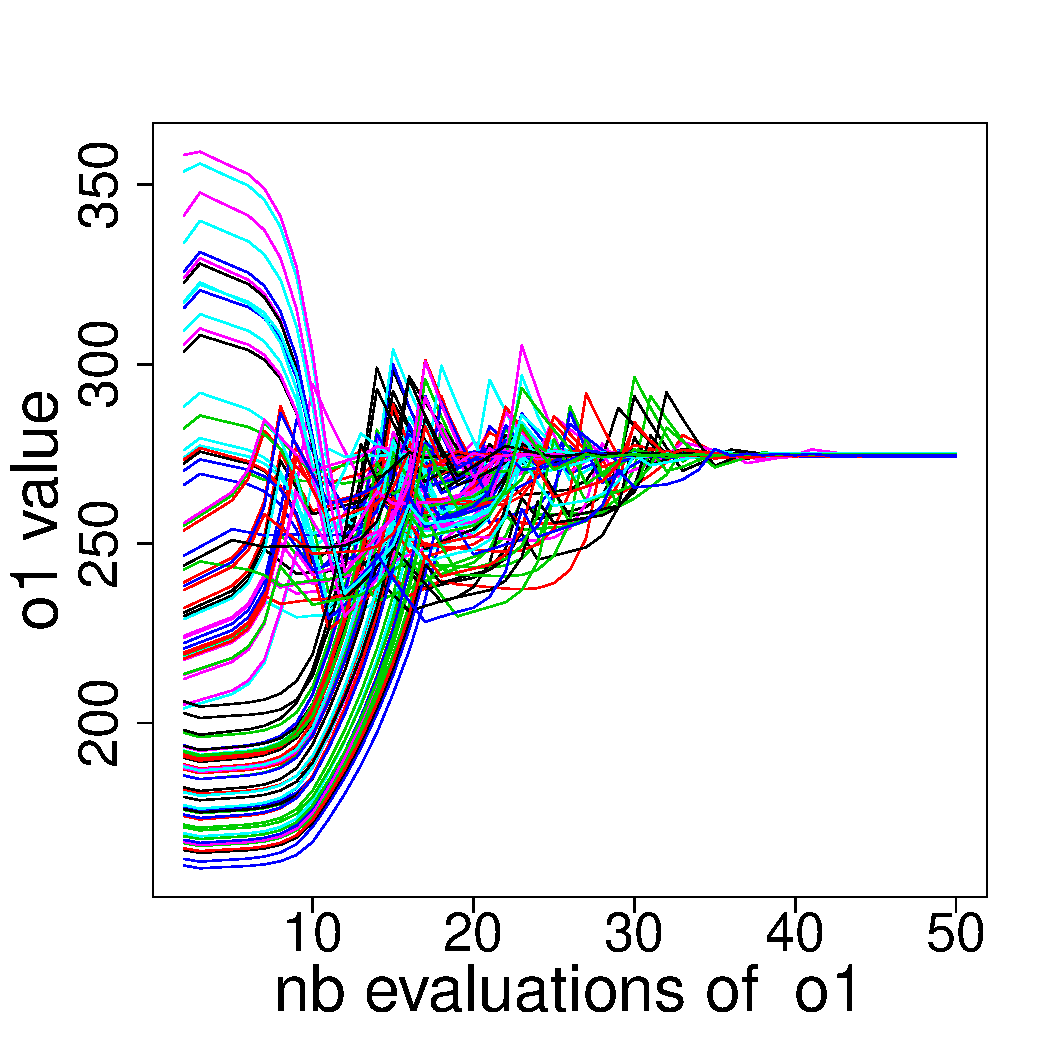
\includegraphics[width = \textwidth]{./R_figs/generated/o1}	
	\end{subfigure}
	\hfill%for spacing
	\begin{subfigure}[b]{0.4\textwidth}
		\centering
		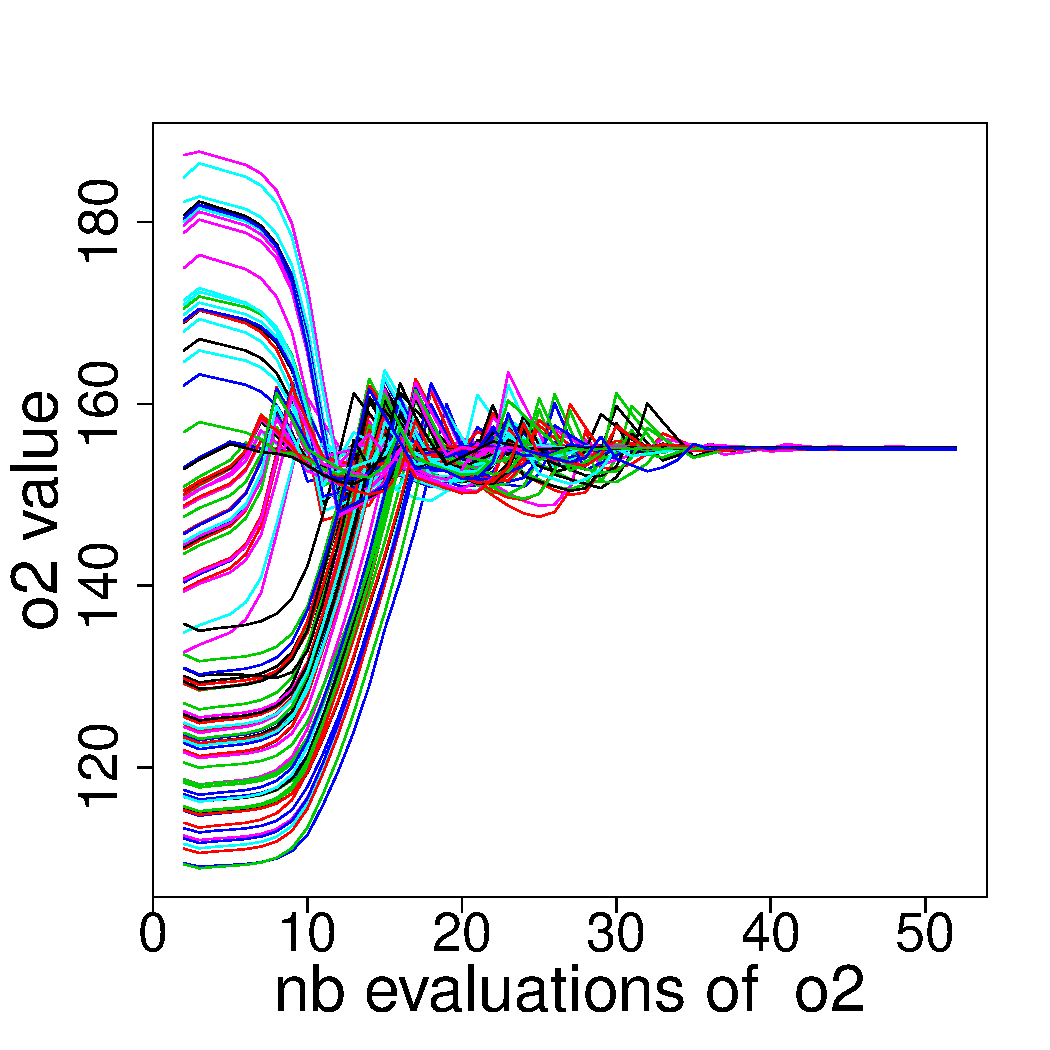
\includegraphics[width = \textwidth]{./R_figs/generated/o2}	
	\end{subfigure}
	\caption{Convergence of the Turbofan objectives for 100 random starting points.}
	\label{snecma_res}
\end{figure}

\section{Viennet1}

The Viennet1 test case is part of a series of problems proposed in \cite{viennet1996multicriteria} to evaluate multi-criteria optimization techniques. This problem involves three objectives. Its analytical formulation is:
\begin{align*}
\text{Minimize } 	&o1 = x^2 + (y-1)^2 \\
								&o2 = x^2 + (y+1)^2 \\
								&o3 = (x-1)^2 + y^2 +2\\
\text{where } 		&x, y \in [-4;4]						
\end{align*}				

\figurename{} \ref{viennet_res} illustrates the convergence of the system toward a valid solution with 100 executions from randomly chosen starting points, using only internal optimization mechanisms.

\begin{figure}[h]

	\begin{subfigure}[b]{0.32\textwidth}
		\centering
		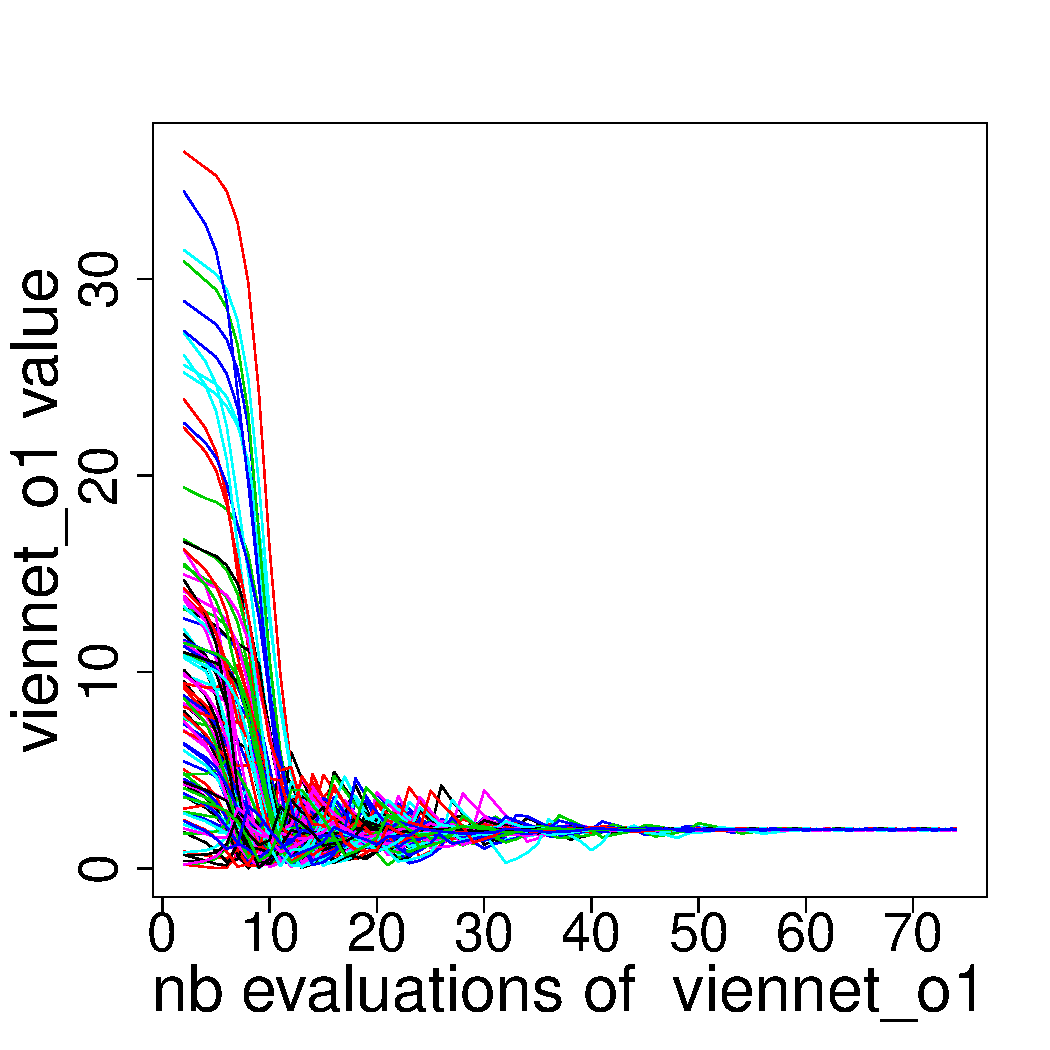
\includegraphics[width = \textwidth]{./R_figs/generated/viennet_o1}	
	\end{subfigure}
	\hfill%for spacing
	\begin{subfigure}[b]{0.32\textwidth}
		\centering
		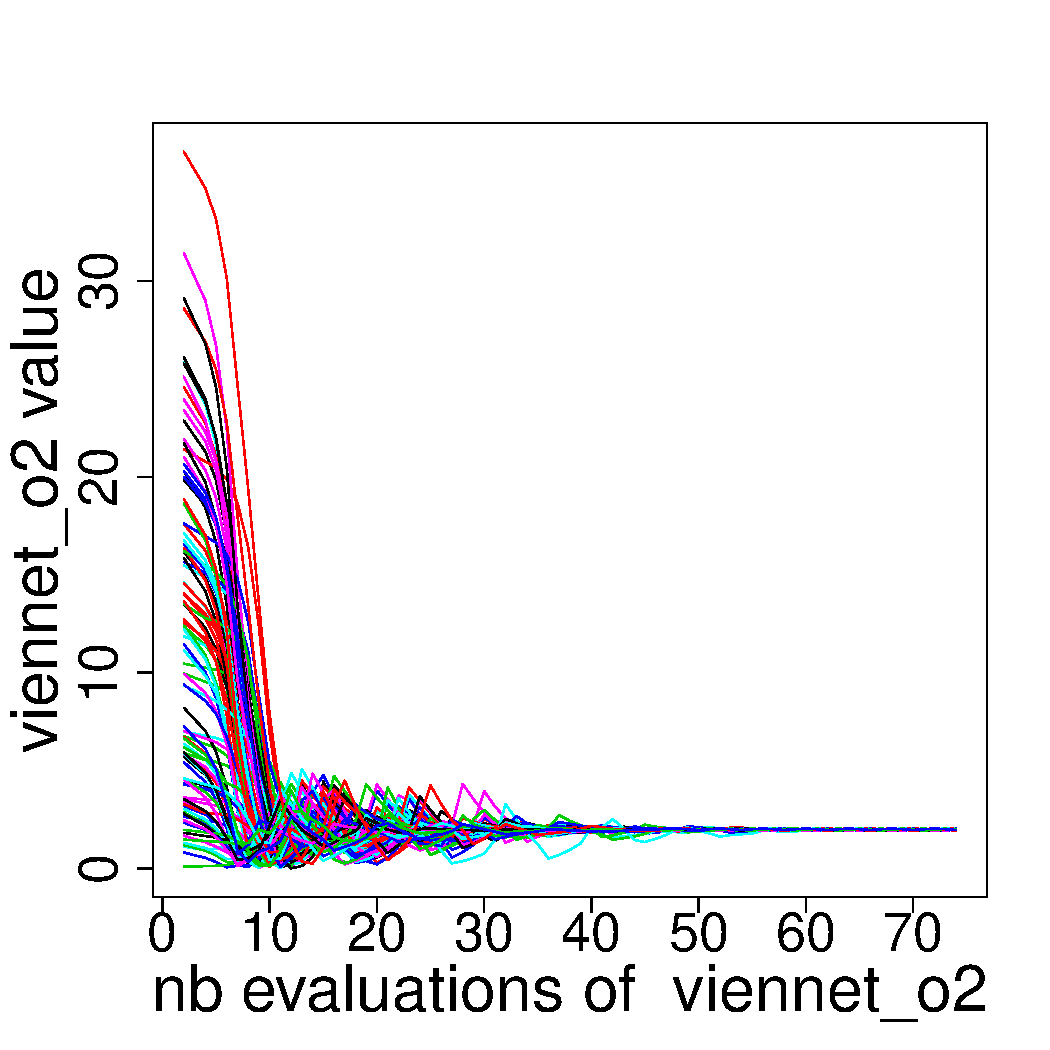
\includegraphics[width = \textwidth]{./R_figs/generated/viennet_o2}	
	\end{subfigure}
	\hfill%for spacing
	\begin{subfigure}[b]{0.32\textwidth}
		\centering
		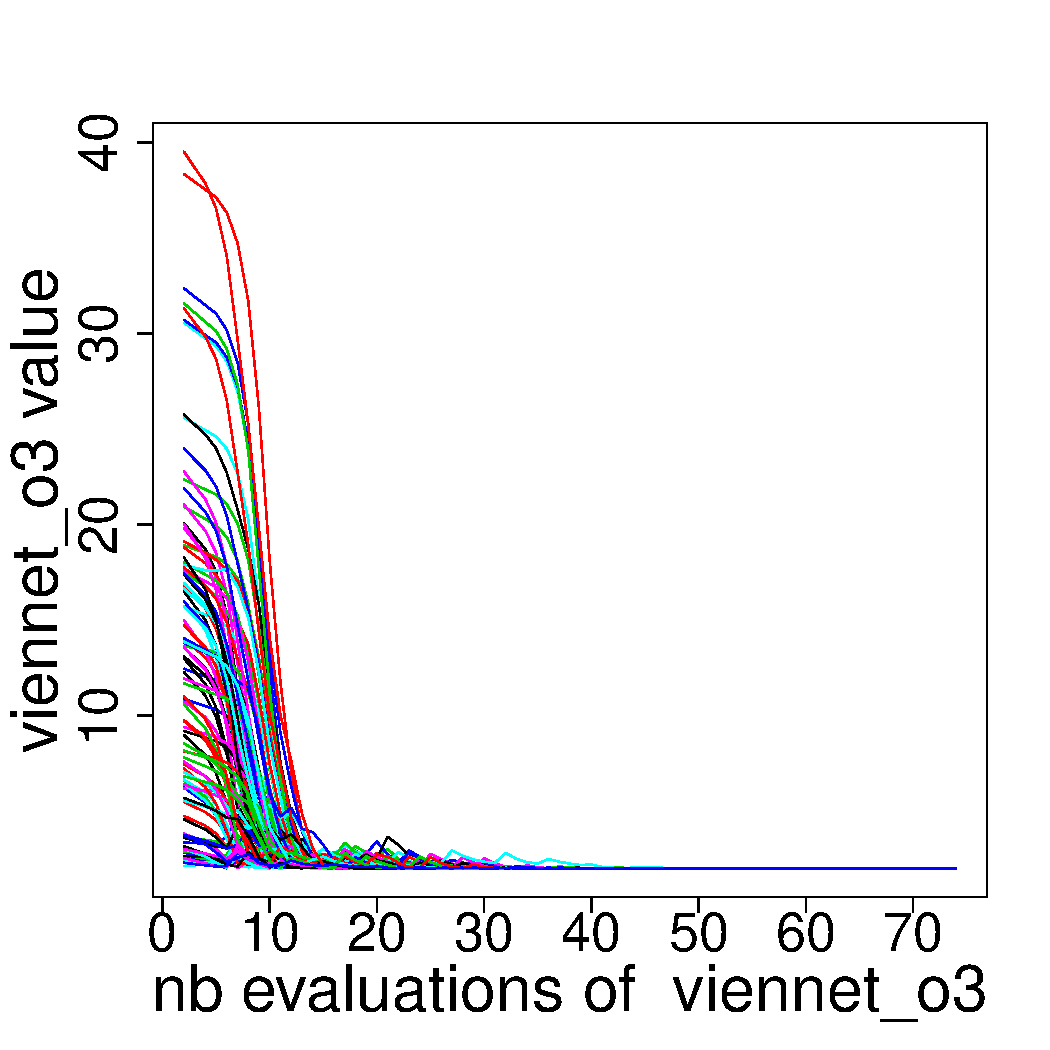
\includegraphics[width = \textwidth]{./R_figs/generated/viennet_o3}	
	\end{subfigure}
	\caption{Convergence of Viennet1 objectives for 100 random starting points.}
	\label{viennet_res}
\end{figure}

\section{Rosenbrock's valley}

Rosenbrock's valley is non-convex function commonly used to test convergence capabilities of an optimization method \cite{Rosenbrock01011960}.

The analytical formulation of this problem (for two dimensions) is 
$$\text{Minimize } f(x,y) = (1-x)^2 + 100(y - x^2)^2$$

The Rosenbrock's valley problem is interesting in the fact that the global minimum is \enquote{hidden} into a narrow parabolic valley. The optimization method must thus get down into the valley and manage to follow its bottom until reaching the global optimum. Consequently it is a very adequate problem to test the cooperative trajectories mechanisms of our system.

The results presented on \figurename{} \ref{rosenbrock_res} are for the two-dimensional version of the problem with a definition domain of [-5; 5] for each \emph{design variable}.

\begin{figure}
\centering
	\begin{subfigure}{0.45\textwidth}
		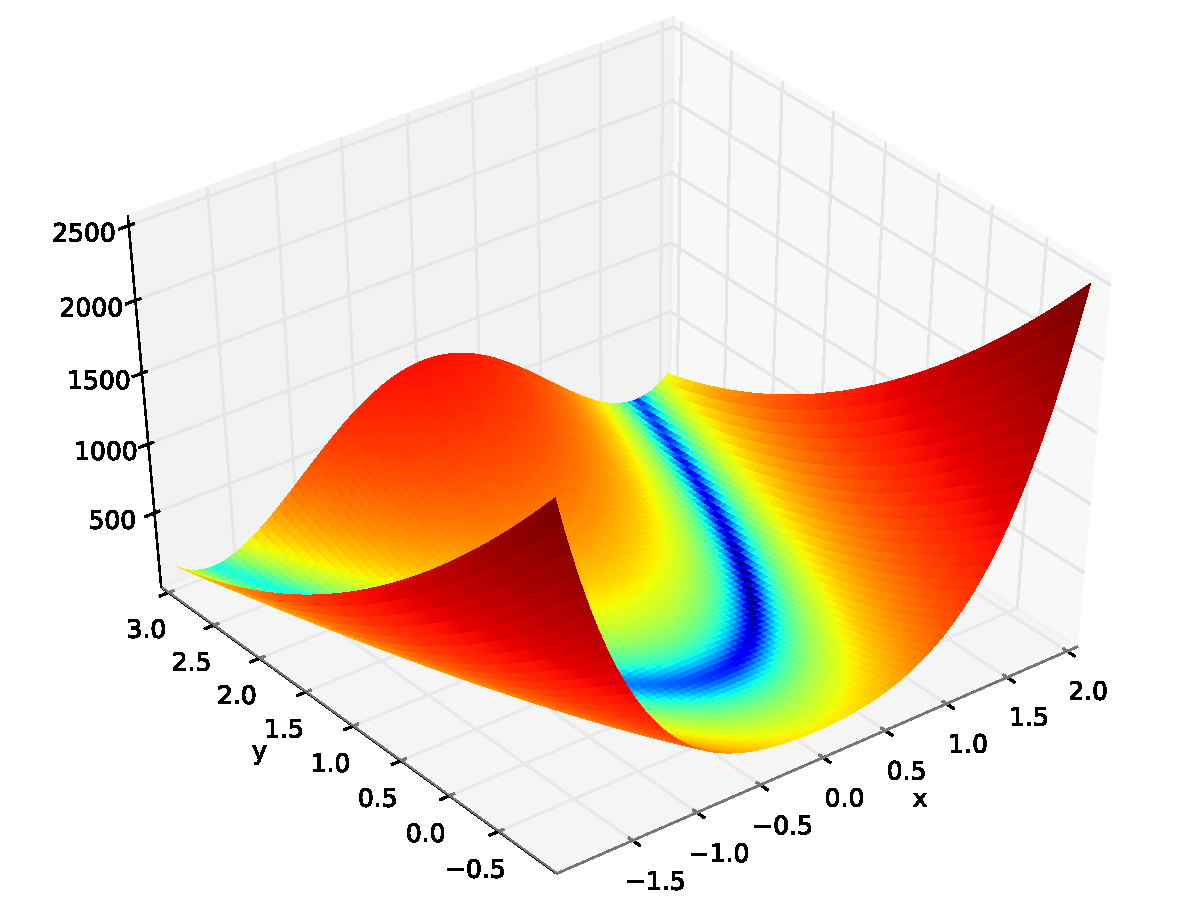
\includegraphics[width=\textwidth]{Rosenbrock_function}
		\caption{Rosenbrock's valley (from \href{http://commons.wikimedia.org/wiki/File:Rosenbrock_function.svg}{Martin Doege}).}\label{rosenbrock_plot}
	\end{subfigure}
	%
	\hfill%for spacing
	%
	\begin{subfigure}{0.45\textwidth}	
		\centering
		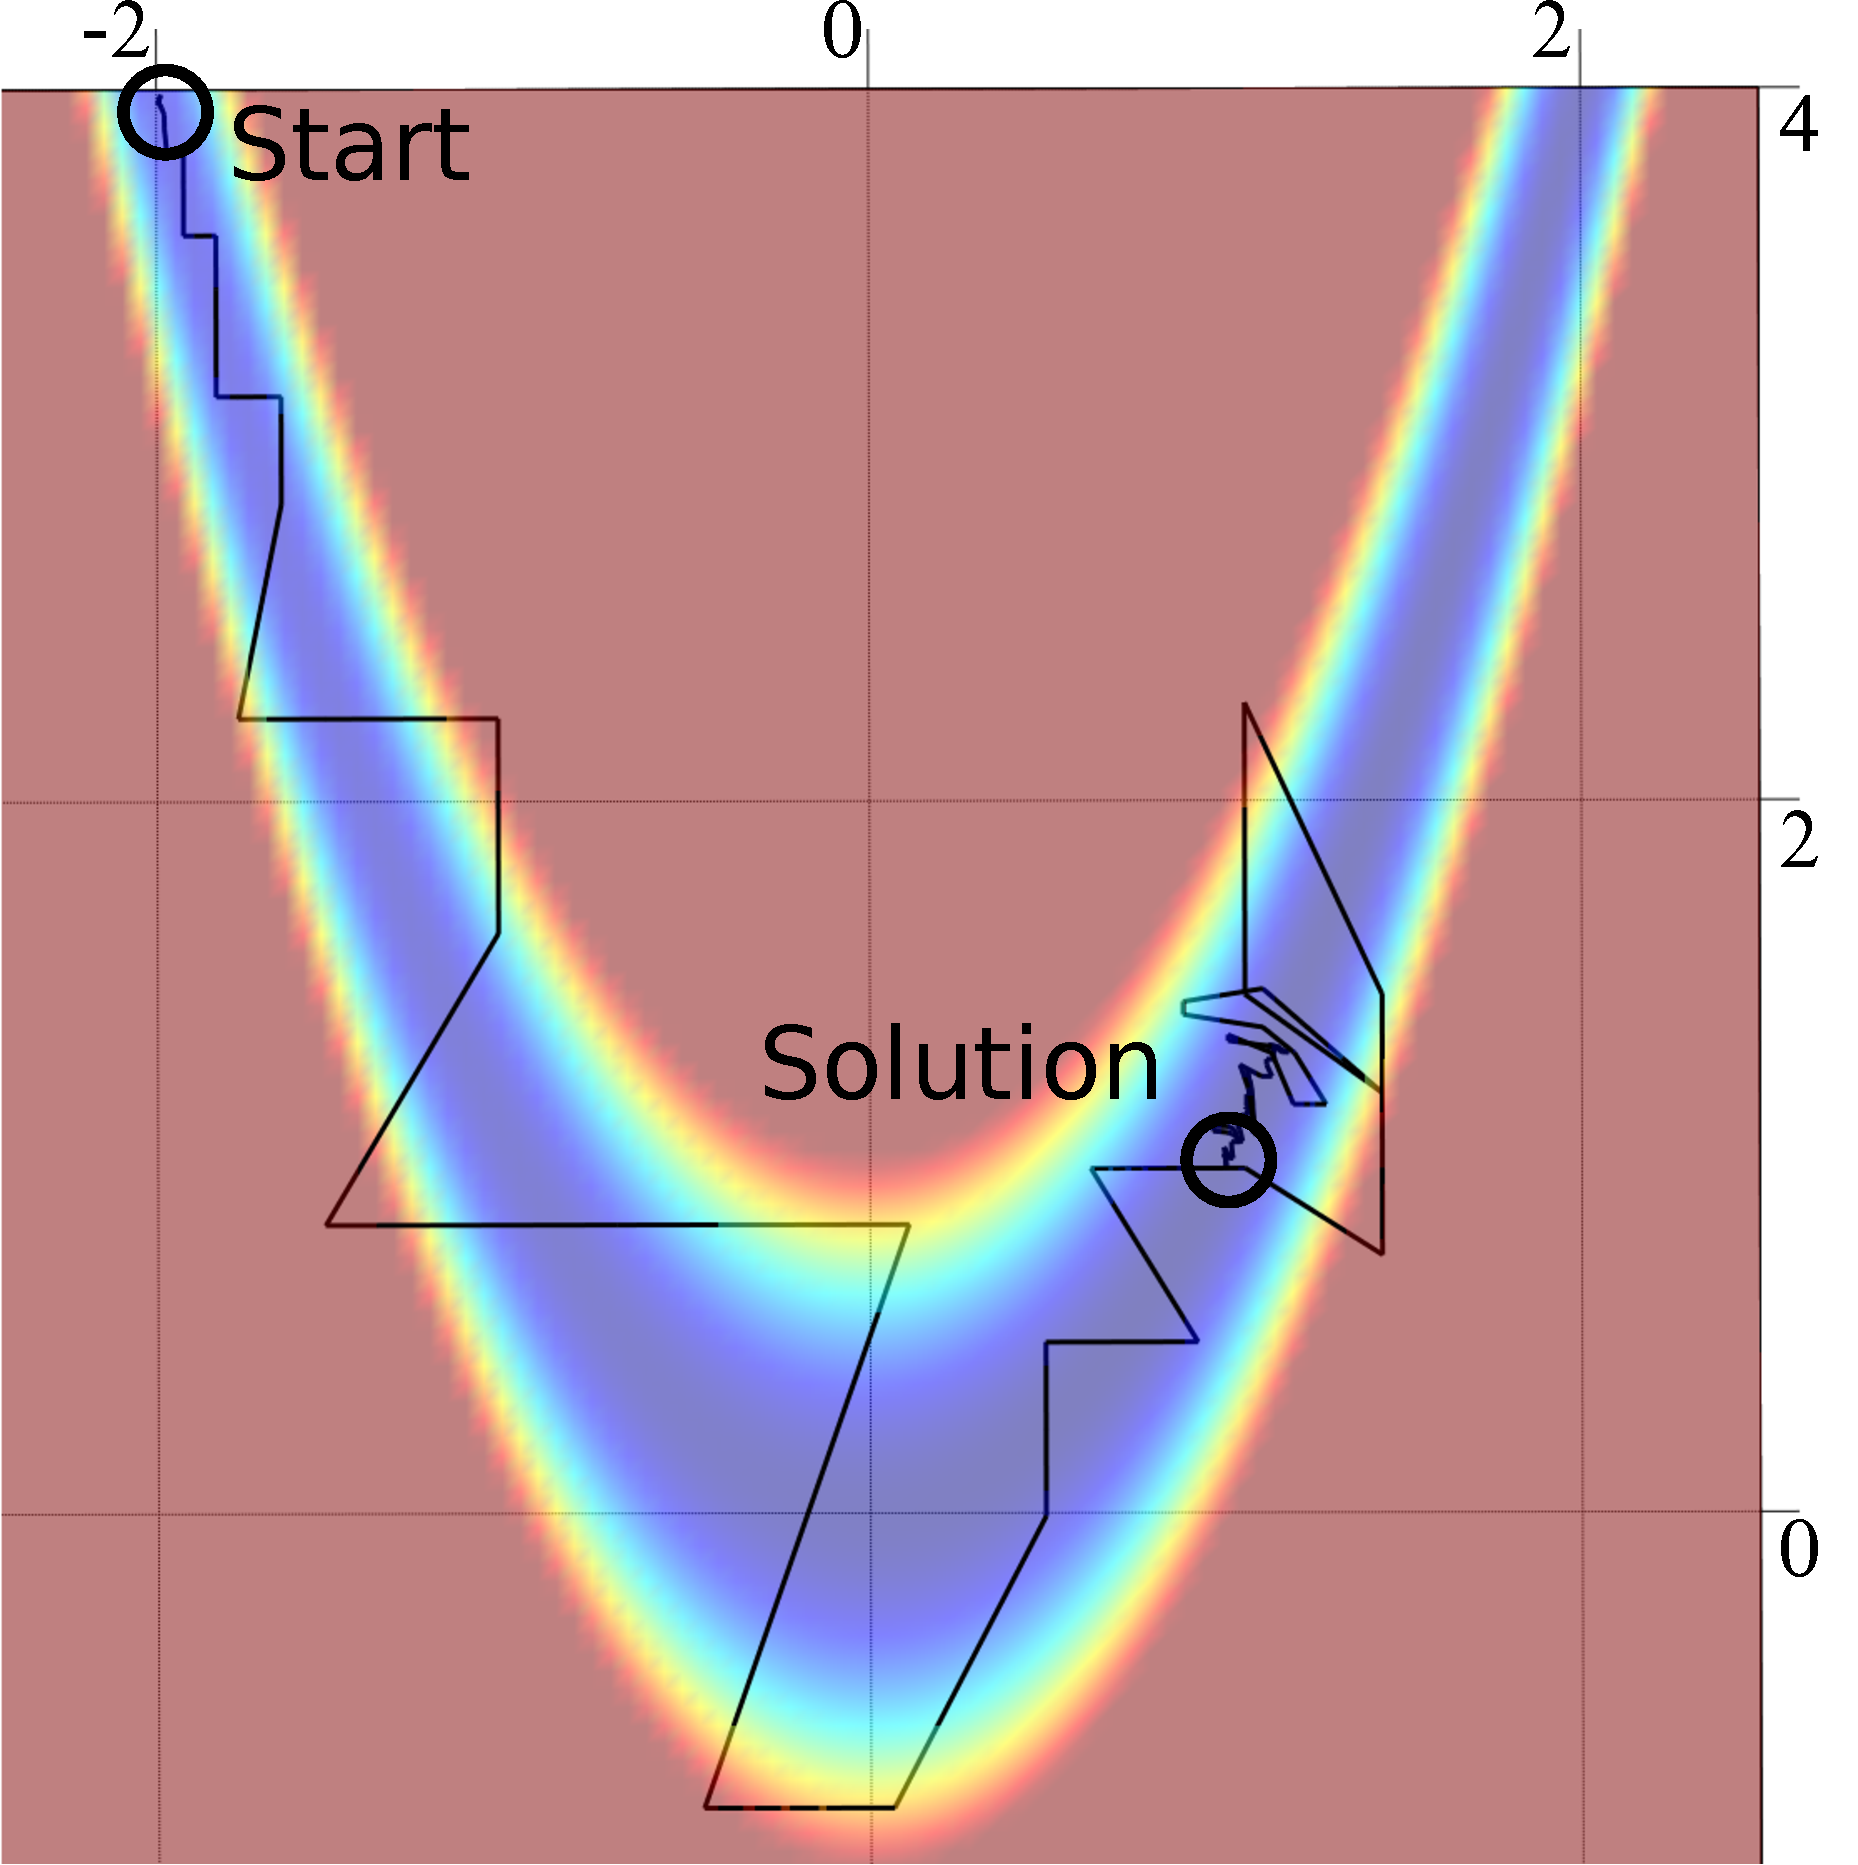
\includegraphics[width=\textwidth]{cooperative_trajectories_example}
		\caption{Example of cooperative trajectories on Rosebrock's valley (starting point (-2, 4)).}\label{collective_traj_rosenbrock_plot}
	\end{subfigure}
	
	\begin{subfigure}{0.4\textwidth}
		\centering
		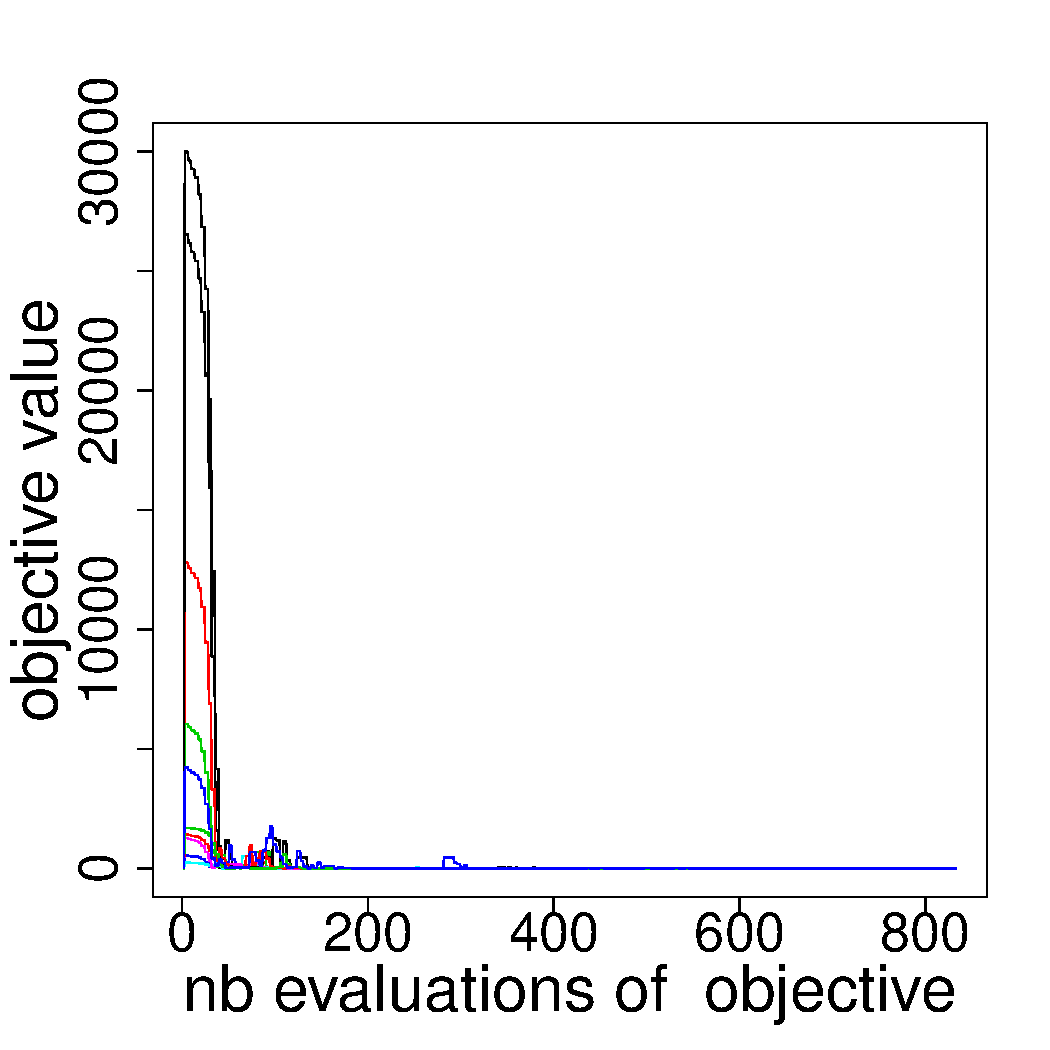
\includegraphics[width = \textwidth]{./R_figs/generated/objective}	
		\caption{Convergence of Rosenbrock objective for 100 random starting points.}\label{rosenbrock_res}
	\end{subfigure}
\caption{Rosenbrock's valley.}
\end{figure}

This problem was also used in \cite{Ilan:1994:MOM:887207} as an application example of the Collaborative Optimization method, presented in chapter \ref{MDO_chapter} (with performances varying from 141 to 1556 total iterations depending on the additional information used).

\section{Alexandrov Problem}

Our last test case is inspired from an academic example taken in literature by Alexandrov \emph{et al}\cite{alexandrov2002analytical}. This example presents many of the commons characteristics of MDO problems: a cycle (albeit converging) and multiple criteria requiring cooperative trajectories. In the original article, the example was used to illustrate some properties of Collaborative Optimization, which we presented earlier, in terms of reformulation. While the paper only gave the structure of the problem, we adapted it with meaningful values and equations.

The mathematical formulation of the problem and the corresponding agent graph can be seen in \figurename{} \ref{alexandrov}. Interestingly, the NDMO representation is quite similar to the one adopted by the original authors of the problem.

\begin{figure}
\centering
	\begin{subfigure}[b]{0.4\textwidth}
		$\begin{array}{c}
			a_1 = (l_1 - a_2)/2 \\
			a_2 = (l_2 - a_1)/2 \\
			min \; \frac{1}{2}(a_1^2 + 10a_2^2 + 5(s-3)^2) \\
			subject \; to \\
			s + l_1 \leq 1 \\
			-s + l_2 \leq -2
		\end{array}$
		\caption{mathematical formulation.}\label{alexandrov:math}
	\end{subfigure}
	\hfill%for spacing
	\begin{subfigure}[b]{0.59\textwidth}
		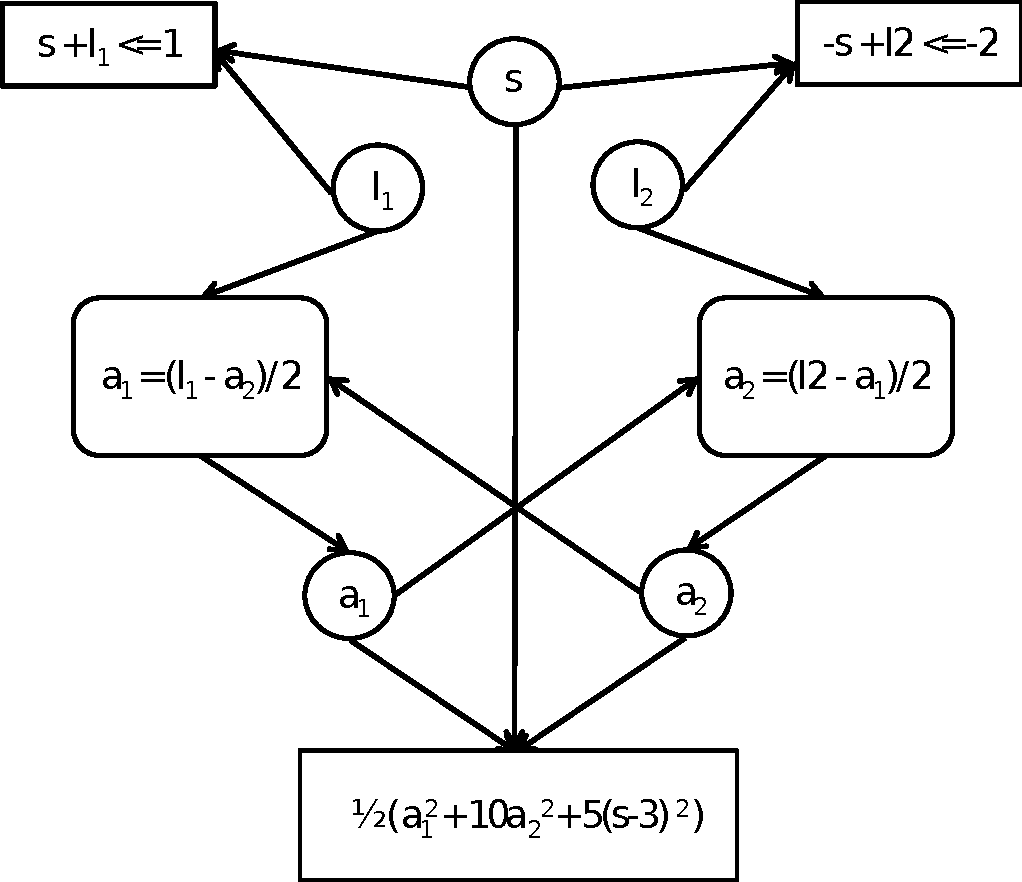
\includegraphics[width=\textwidth]{testcases-Alexandrov}%screen_Alexandrov}%}
		\caption{corresponding agent graph.}\label{alexandrov:graph}
	\end{subfigure}
\caption{Alexandrov problem.}\label{alexandrov}
%\vspace{-20pt}
\end{figure}

On \figurename{} \ref{alexandrov_res_one}, the behavior of the \emph{design variables} agents l1, l2 and s, as well the evolution of the objective, can be observed on one instance of the problem with random starting points.

\begin{figure}
\centering
	\begin{subfigure}[b]{0.4\textwidth}
		\centering
		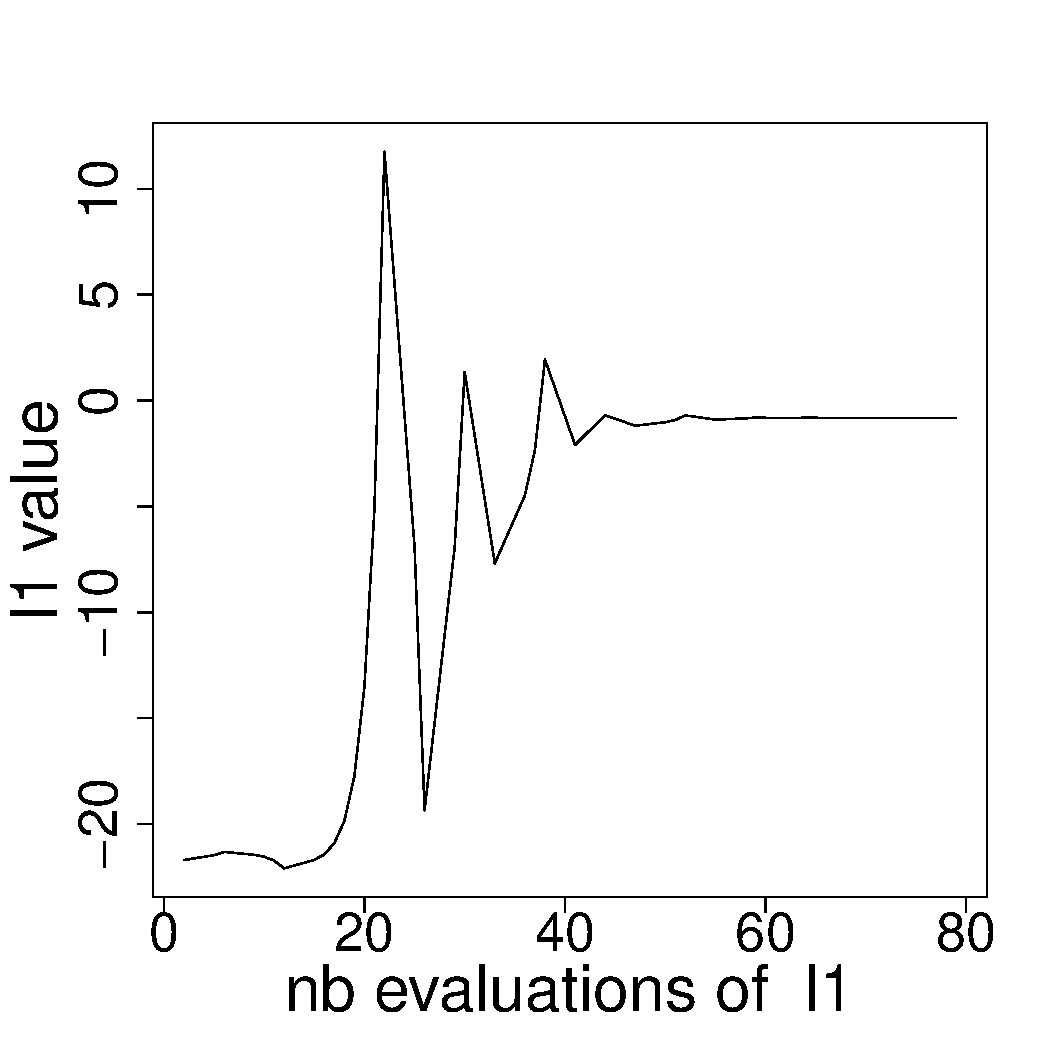
\includegraphics[width=\textwidth]{./R_figs/generated/l1_one_run}
		%\vspace{-20pt}
		\label{alexandrov_res_one:l1}
	\end{subfigure}
	\begin{subfigure}[b]{0.4\textwidth}
		\centering
		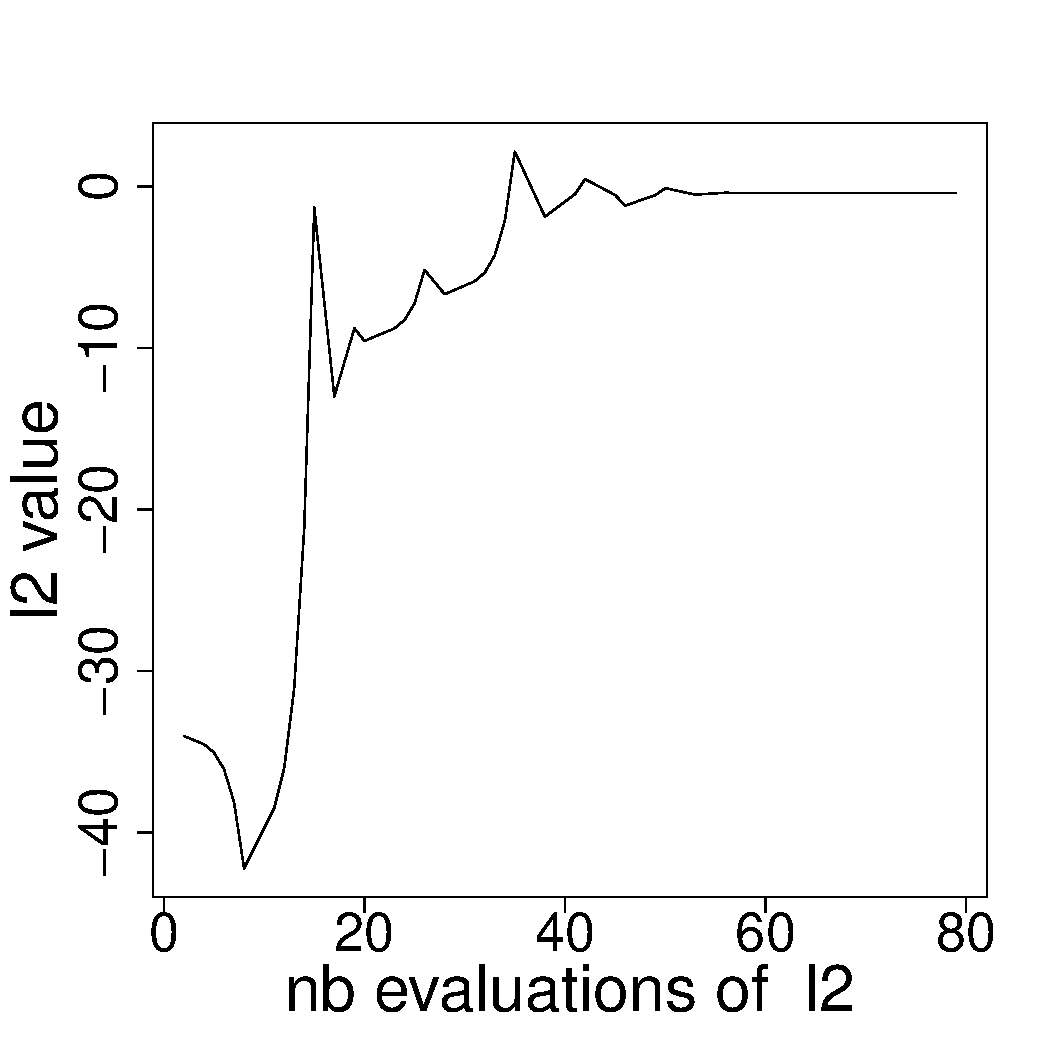
\includegraphics[width=\textwidth]{./R_figs/generated/l2_one_run}
		%\vspace{-20pt}
		\label{alexandrov_res_one:l2}
	\end{subfigure}
	\vspace{-20pt}
	\\
	\begin{subfigure}[b]{0.4\textwidth}
		\centering
		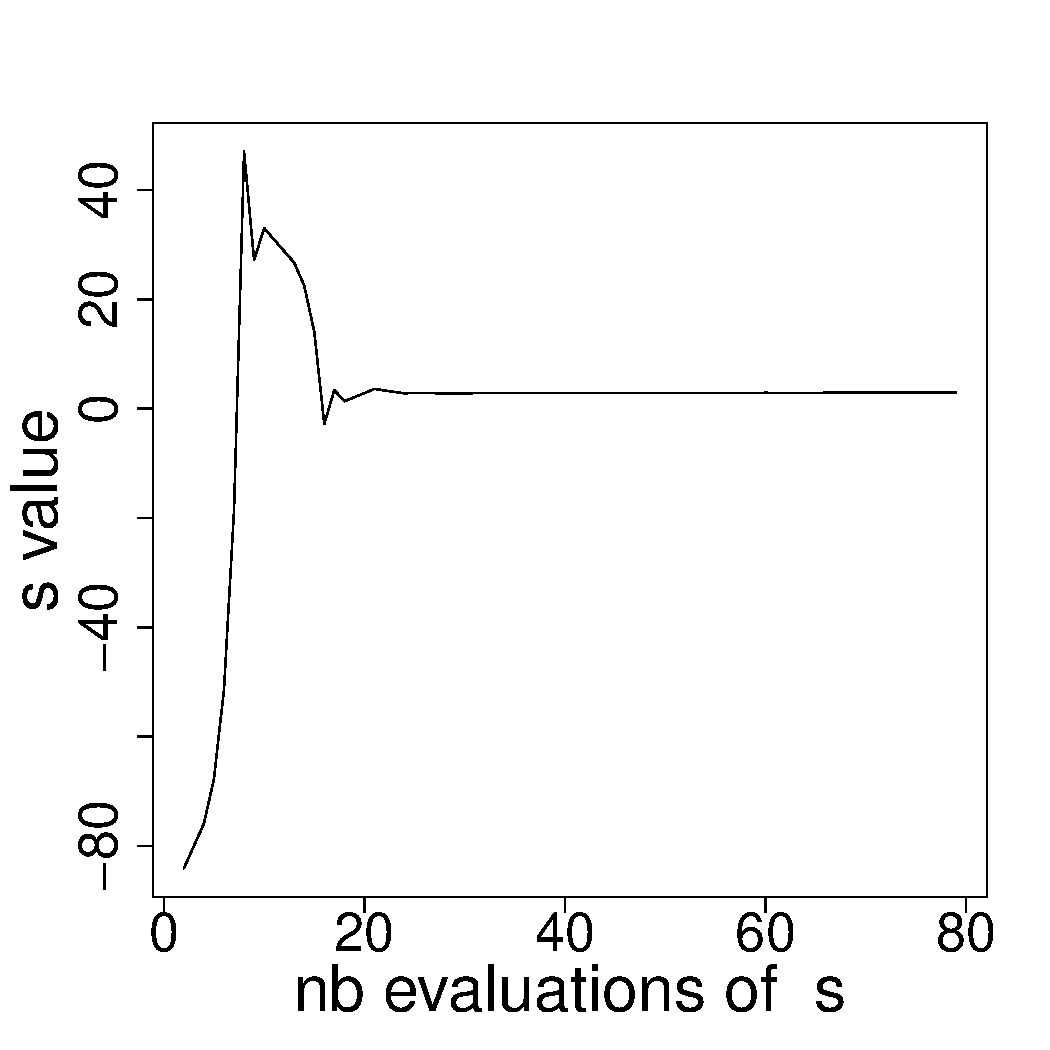
\includegraphics[width=\textwidth]{./R_figs/generated/s_one_run}
		%\vspace{-20pt}
		\label{alexandrov_res_one:s}
	\end{subfigure}
	\begin{subfigure}[b]{0.4\textwidth}
		\centering
		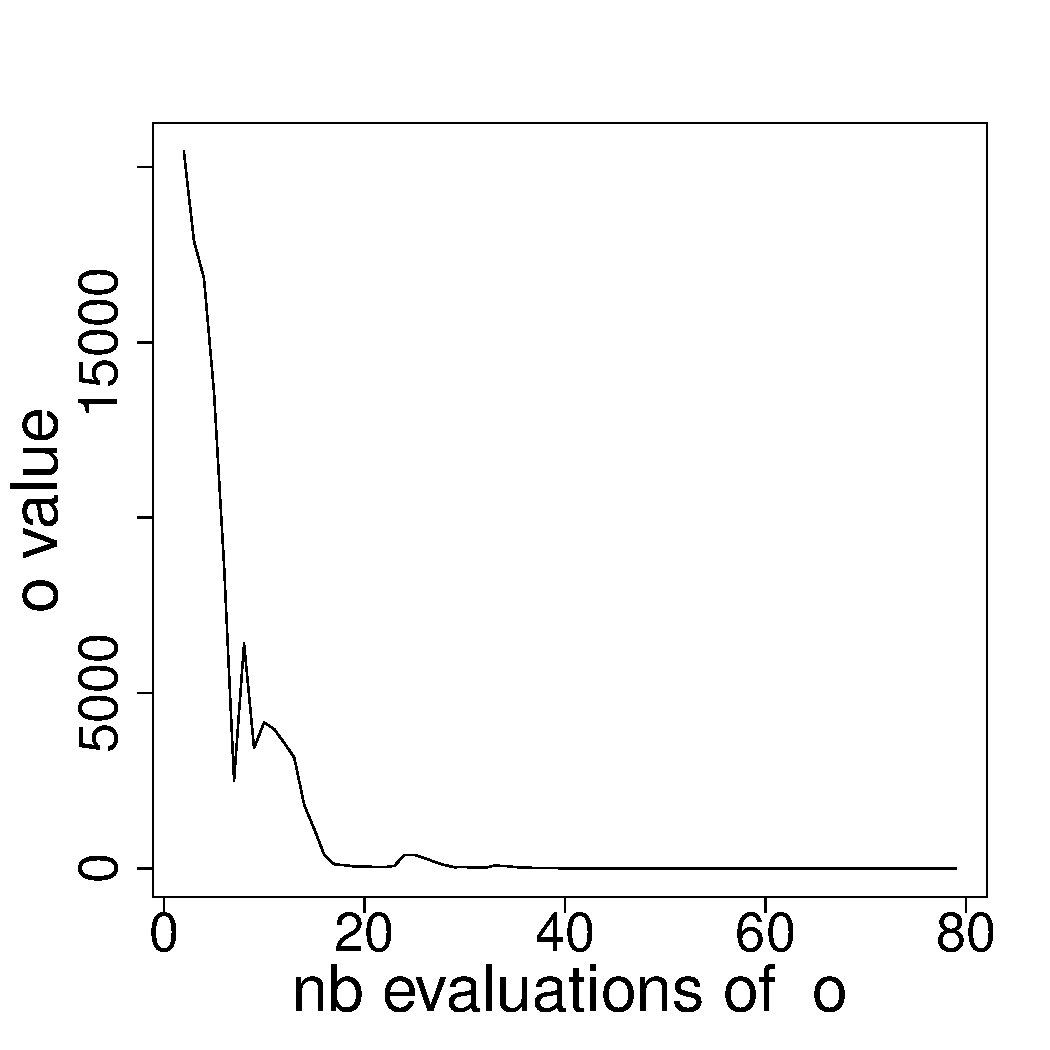
\includegraphics[width=\textwidth]{./R_figs/generated/o_one_run}
		%\vspace{-20pt}
		\label{alexandrov_res_one:o}
	\end{subfigure}
	
	\caption{Alexandrov agents behavior.}
	\label{alexandrov_res_one}

\end{figure}

On \figurename{} \ref{alexandrov_res}, we show the evolution of the objective over 100 iterations with starting points for each \emph{design variable} randomly drawn over the interval [-100; 100]. We can see how the system converges towards the same optimum despite the wildly different initial conditions.

\begin{figure}
\centering
	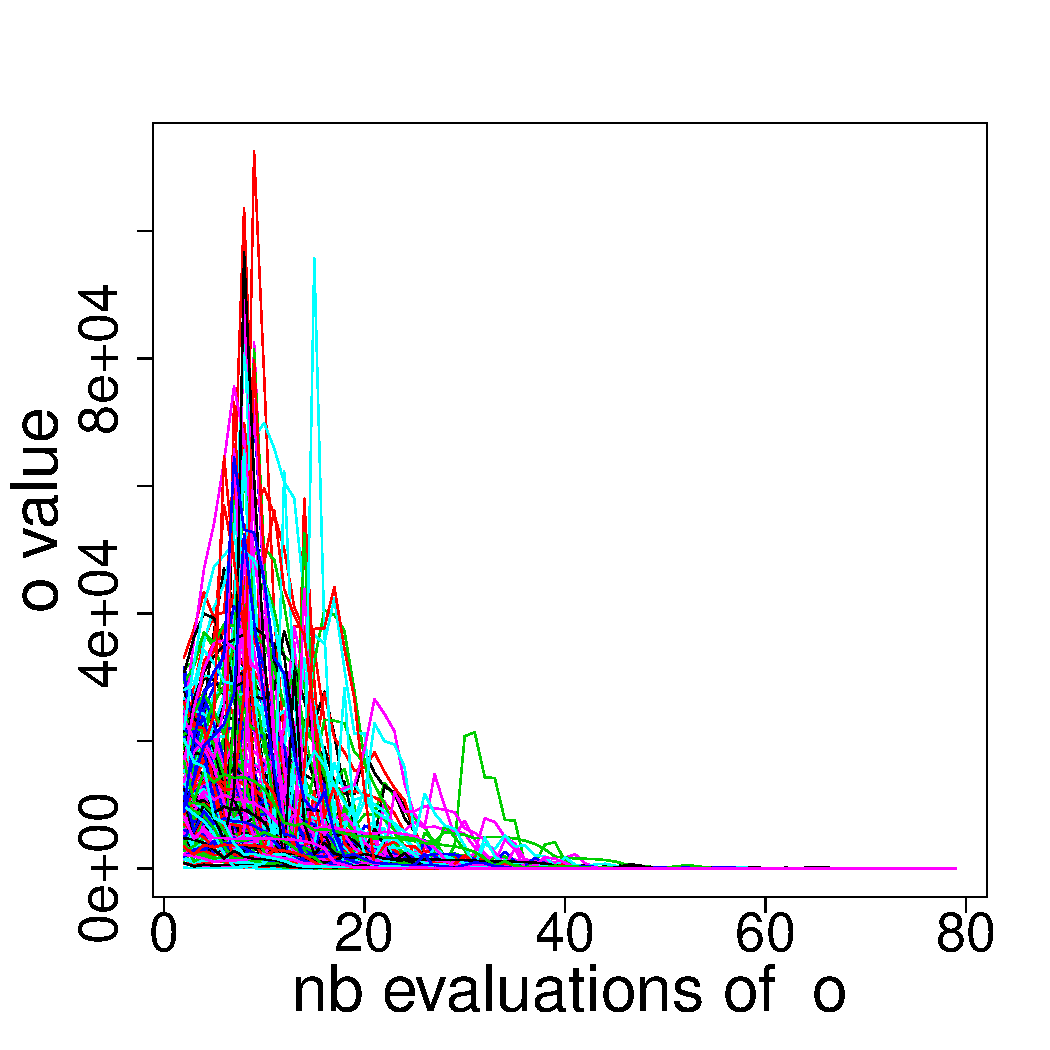
\includegraphics[width=0.4\textwidth]{./R_figs/generated/o}
	\caption{Convergence of the Alexandrov objective for 100 random starting points.}
	\label{alexandrov_res}
\end{figure}

\section{Analysis of Academic Test Cases}

In this section we presented several academic test cases exhibiting classical properties of complex continuous optimization problems. We shown how the system was able to consistently converge on each test case toward an optimum solution, for multiple starting points.

Summarized results illustrating the convergence of the system. are presented on \tablename{} \ref{experiments_res}. The first group of values represents the number of evaluations which was needed for respectively 10\%, 50\% and 90\% of the instances to find the best solution. The second group represent the average distance to the best solution (truncated at $10^{-3}$) among all instances at different times (0\% being the start 100\% being the end of the solving in the worst case).

\begin{table}
\caption{Summary of experiments results for the tests cases}\label{experiments_res}

\centering
\begin{tabular}{cccc|cccc}
	\toprule
		& \multicolumn{3}{c|}	{nb. evaluations to best}
		& \multicolumn{4}{c}	{average distance to best} \\
	\cline{2-8}
		&	10\%		& 	50\%	&		90\%	&	0\% (start)		& 	30\%	&		60\%	&	100\% (end)\\
	\toprule
	Turbofan\_o1 & 22 & 38 & 50 & 67.654 & 21.563 & 1.78 & 0.313\\
	Turbofan\_o2 & 14 & 23 & 32 & 23.876 & 2.485 & 0.387 & 0.101\\
	\midrule
	Viennet\_o1 & 8 & 17 & 29 & 8.514 & 0.458 & 0.033 & 0.021\\
	Viennet\_o2 & 9 & 15 & 27 & 9.412 & 0.37 & 0.043 & 0.021\\
	Viennet\_o3 & 9 & 14 & 23 & 10.622 & 0.102 & 0.001 & 0.0	\\
	\midrule
	Rosenbrock & 19 & 47 & 56 & 13749.427 & 123.44 & 4.564 & 2.201\\
	\midrule
	Alexandrov & 36 & 52 & 70 & 13109.169 & 1236.501 & 15.434 & 0.059\\
	\bottomrule
\end{tabular}

\end{table}

These results tend to validate the correctness of our approach, proving that the conjunction of the agents nominal behaviors and cooperative mechanisms allows to solve correct solution to diverse optimization problems.

We will now present the second part of our validation, by making experiment on larger test cases in order to validate the system behavior on complex problem and to compare the performances of our system with other complex optimization methods.

\section{Optimization under Uncertainties}

While it is not the focus of our system, we worked with our partners of the ID4CS project to illustrate the uncertainties propagation capabilities presented in section \ref{mas_uncertainties}. To this end, we were provided with a preliminary aircraft design test case inspired from \cite{scholz2008preliminary}. The test case is declined into two versions: a deterministic optimization problem and an optimization problem under uncertainties.

The deterministic version is the following:

\begin{align*}
	\text{min }& f = \dfrac{2 g^3 L \sigma S_d}{C_L (A M^m {\sigma}^n \eta_{P,Cr} E)^2 \sigma (H)} \dfrac{1}{ \left( \dfrac{m_{MTO}}{S_W} \right) } \left(\dfrac{P_{TO}}{m_{MTO}}\right)^3  \\
	\text{s.t. } & g_1 = \dfrac{m_{MTO}}{S_W} - \dfrac{k_L \sigma C_{L, max, L} S_{LFL}}{ m_{ML}/m_{MTO}}\leq 0 \\
						&	g_2 = \dfrac{k_{TO} V g }{s_{TOFL} \sigma C_{L, max, TO} \eta_{P, TO}} - \dfrac{P_{TO}/m_{MTO}}{m_{MTO}/S_W} \leq 0\\
						&	g_3 = V_{CR}\dfrac{V_{md}}{E \eta_{P, CR} A M^m {\sigma}^n} \sqrt{\dfrac{\pi A e {\rho}_0 \sigma(H)g}{4 E_{max}}} - \dfrac{P_{TO}}{M_{MTO}} \sqrt{\dfrac{m_{MTO}}{S_W}} \leq \\
\end{align*}

where $\dfrac{m_{MTO}}{S_W}$ and $\dfrac{P_{TO}}{m_{MTO}}$ are the two design variables of the problem, representing respectively the power/mass ratio and the wing loading of the aircraft, and the other values are constants. The three constraints concern respectively the takeoff length, landing length and cruising speed. The solution to the deterministic problem is $\dfrac{m_{MTO}}{S_W} = 377$ and $\dfrac{P_{TO}}{m_{MTO}} = 187$, for $f = 2.15E+08$.

In the version with uncertainties, normal distribution laws are associated with some variables of the problem. The variables and associated uncertainties are shown in \tablename{} \ref{uncertainties_values}

\begin{table}
\caption{Uncertainties associated with the variables}\label{uncertainties_values}
\centering
\begin{tabular}{lrr}
\toprule
Variable & Expected value & Standard deviation\\
\midrule
$C_{L,max,L}$			&	2.50		&	0.250	\\
$C_{L, max, TO}$	&	2.10		&	0.210	\\
$E$								&	12.49	&	1.249	\\
$\eta_{P, CR}$			&	0.86		&	0.086	\\
\bottomrule
\end{tabular}
\end{table}

The new objective is not to minimize $f$ but to minimize $E(f)$, the expected value of the function. The new constraints are $P(g_i \leq 0) \geq 0.9, \; \forall i \in \{1, 2, 3\}$.

We slightly adapted our MAS to mimic a classical sequential optimization scheme. The basic idea of this type of method is to start by doing a deterministic optimization of the problem and, when the optimization has converged, to switch to an optimization under uncertainties using the deterministic solution point as a starting point. For our MAS, we instantiated this method by making the agents start doing a deterministic optimization. When a certain convergence condition is detected, the agents automatically switch to  optimization under uncertainties. A difference is that the system is not interrupted between the deterministic optimization and optimization under uncertainties. The agents handle the transition automatically by switching to uncertain values.

The solution to the problem under uncertainties is $\dfrac{m_{MTO}}{S_W} = 329$ and $\dfrac{P_{TO}}{m_{MTO}} = 244$

For the uncertainties propagations, the agents are provided with Monte-Carlo propagators. These propagators draw 50000 random values on the inputs following the uncertainties associated with each input, and return a set of points for each outputs. The constraints and objectives can directly use these sets of points, as explained in chapter \ref{mas_uncertainties}.

The trajectory of the system is shown on \figurename{} \ref{sequential_optim_fig}. The red dashed curves represent the deterministic constraints. The blue and green circles represent respectively the deterministic and robust solution points. The starting point (300, 300) is indicated by the letter S. We can see on the figure how, in the first part, the system converges toward the deterministic solution point and, on the second part, how it switches to uncertainties and changes its direction to converges on the robust solution point.

\begin{figure}
\centering
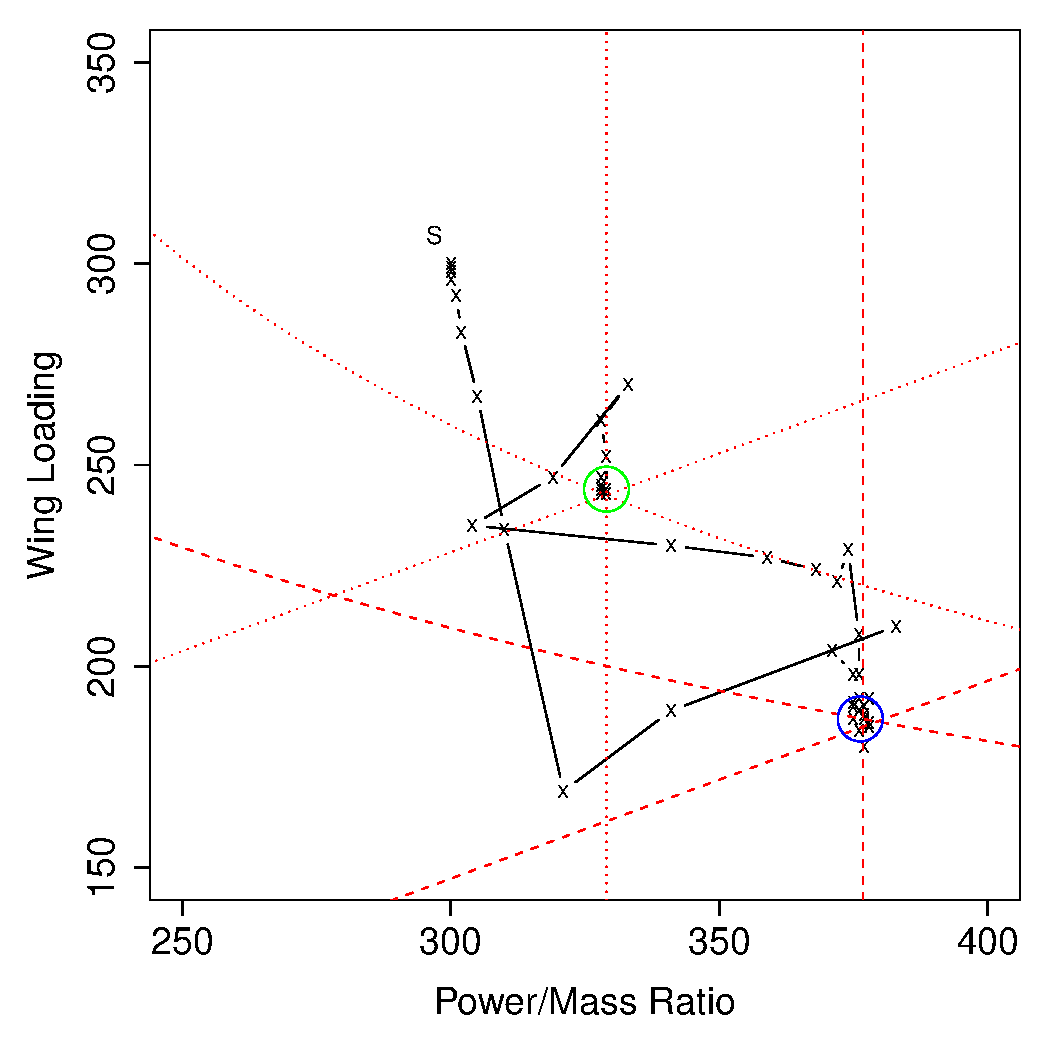
\includegraphics[width=0.7\textwidth]{uncertainties/uncertainties}
\caption{Sequential optimization trajectory.}\label{sequential_optim_fig}
\end{figure}

\section{Adaptation to Perturbations}

\subsection{Perturbated Alexandrov Problem}
 
On \figurename{} \ref{alexandrov_res_pert}, we can observe the reaction of the multi-agent system to a perturbation. During the solving of the previous experimentation on the problem, we changed the threshold of the constraint $s + l_1 \leq 1$ to $s + l_1 \leq -4$ (the change is indicated by a dotted line on the charts). The system dynamically adapts to the constraint changed and converges towards a new solution which satisfies the updated constraint.

\begin{figure}[]
\centering
	\begin{subfigure}[b]{0.4\textwidth}
		\centering
		\includegraphics[width=\textwidth]{./R_figs/generated/l1_pertubated}
		\label{alexandrov_res_pert:l1}
	\end{subfigure}
	\begin{subfigure}[b]{0.4\textwidth}
		\centering
		\includegraphics[width=\textwidth]{./R_figs/generated/l2_pertubated}
		\label{alexandrov_res_pert:l2}
	\end{subfigure}

	\begin{subfigure}[b]{0.4\textwidth}
		\centering
		\includegraphics[width=\textwidth]{./R_figs/generated/s_pertubated}
		\label{alexandrov_res_pert:s}
	\end{subfigure}
	\begin{subfigure}[b]{0.4\textwidth}
		\centering
		\includegraphics[width=\textwidth]{./R_figs/generated/o_pertubated}
		\label{alexandrov_res_pert:o}
	\end{subfigure}
	
	\caption{Alexandrov agents behavior with perturbation (constraint change at dotted line).}
	\label{alexandrov_res_pert}
	
\end{figure}

\subsection{Perturbated Turbofan Problem}

\begin{figure*}
\centering

	\begin{subfigure}[b]{0.32\textwidth}
		\centering
		\includegraphics[width=\textwidth]{./R_figs/generated/turbofan_perturbated_pi_c}
		\label{turbofan_res_pert:pi_c}
	\end{subfigure}
	\begin{subfigure}[b]{0.32\textwidth}
		\centering
		\includegraphics[width=\textwidth]{./R_figs/generated/turbofan_perturbated_o1}
		\label{turbofan_res_pert:o1}
	\end{subfigure}
	\begin{subfigure}[b]{0.32\textwidth}
		\centering
		\includegraphics[width=\textwidth]{./R_figs/generated/turbofan_perturbated_c1}
		\label{turbofan_res_pert:c1}
	\end{subfigure}

	\begin{subfigure}[b]{0.32\textwidth}
		\centering
		\includegraphics[width=\textwidth]{./R_figs/generated/turbofan_perturbated_bpr}
		\label{turbofan_res_pert:bpr}
	\end{subfigure}
	\begin{subfigure}[b]{0.32\textwidth}
		\centering
		\includegraphics[width=\textwidth]{./R_figs/generated/turbofan_perturbated_o2}
		\label{turbofan_res_pert:o2}
	\end{subfigure}
	\begin{subfigure}[b]{0.32\textwidth}
		\centering
		\includegraphics[width=\textwidth]{./R_figs/generated/turbofan_perturbated_c2}
		\label{turbofan_res_pert:c2}
	\end{subfigure}
	
	\caption{Turbofan agents behavior with perturbations (changes at dotted lines).}
	\label{turbofan_res_pert}
\end{figure*}


On \figurename{} \ref{turbofan_res_pert}, we illustrate the adaptation capabilities of the system by subjecting turbofan problem we introduced previously to a series of both strong and faster successive small changes to the problem topology (each perturbation is indicated by a dotted line). \\
First we create strong changes by modifying simultaneously both a constraint and the definition domain of $pi\_c$:
\begin{description}
\item[a.] $c1$ changed from $s <= 155$ to $s <= 165$, max bound of $pi\_c$ changed from 40 to 50
\item[b.] $c1$ changed from $s <= 165$ to $s <= 145$, max bound of $pi\_c$ changed from 50 to 30
\end{description}
 Then milder perturbations by only changing the definition domain of the variable:
\begin{description}
\item[c.] max bound of $pi\_c$ changed from 30 to 35
\item[d.] max bound of $pi\_c$ changed from 35 to 40
\item[e.] max bound of $pi\_c$ changed from 40 to 45
\end{description}
The experiments show that the system consistently reacts to these perturbations by adapting itself in order to find a new solution for the modified problem.

\chapter{Comparison with Existing Methods}

In this chapter we provide a comparison of our MAS with existing MDO methods. This comparison is based on the work of \cite{perez2004evaluation, Yi2008}. These two works are complementary as both of them concern a common subset of representative MDO methods: MDF, IDF, CSSO, BLISS and CO.

The work of \cite{perez2004evaluation} presents an analysis of these methods based on two test cases and rank them on multiple criteria: \emph{Accuracy, Efficiency, Transparency, Simplicity, Portability}.

The analysis of \cite{Yi2008} is based on different criteria, concentrating on the performances regarding the number of functions calls and the additional informations required by each methods. An interesting aspect of this comparison is that it provides several mathematical test cases on which the methods are applied.

For our evaluation we use test cases provided by both works and compare the performances of our system to the existing MDO methods. We then provide a comparison synthesis based on the criteria and analysis presented in \cite{perez2004evaluation}.

In order to obtain comparable results with MDO methods, we adopted a problem modeling based on the disciplines division proposed in these works. To this end, we considered that, for each test case, the natural formulation of the problem matched the proposed disciplines division. Consequently, for each test case, the mathematical models represented by our model agents correspond to the proposed disciplines.

\section{Comparison Criteria}

For our comparisons we use the criteria proposed in \cite{perez2004evaluation}, which are defined as follow:
\begin{compactitem}
\item \emph{Accuracy}: the quality of the solution proposed by the method, based on the distance between the proposed solution and the real optimal values.
\item \emph{Efficiency}: the computational cost to find the proposed solution, based on the number of disciplinary evaluations.
\item \emph{Simplicity}: the ease to instantiate and apply the method to different problems, based on the number of optimizers and variables required to implement the examples.
\item \emph{Transparency}: the capability to understand, modify or extend the method.
\item \emph{Portability}: the feasibility to apply the method in the context of an existing work organization, based on the distributivity capabilities of the method.
\end{compactitem}
 
The \emph{Accuracy} criterion reflects the aptitude of the method to find the input values corresponding to the optimum of the problem.
 
The \emph{Efficiency} criterion concerns the computational cost required by the method to provide its solution. When counting the number of evaluation calls, a distinction is made between discipline evaluations and full problem evaluations, the latter being considered considerably more costly than the former. Our MAS does not require any full problem evaluation, using only disciplines evaluations.
 
The \emph{Simplicity} criterion concerns the amount of work required to instantiate the method to suit different optimization problem. The original authors chose to evaluate this criterion using to measures: the number of optimizers involved and the number of additional variables required by the method.

The \emph{Transparency} criterion is the less well-defined and can be perceived as somewhat subjective. The original authors give as an example that \enquote{a probability-based method can be seamlessly integrated into a transparent formulation, which does not require major changes of the architecture to accomplish the integration.}

The \emph{Portability} criterion concerns the feasibility to integrate the method into an existing organizational structure. This evaluation criterion is based on the capabilities of the method to divide the concerns to match existing expert teams or specializations.

\section{Comparison Problem 1}

Our first comparison test case comes from \cite{perez2004evaluation}. It was originally introduced in \cite{sellar1996response} to study the performances of the CSSO method. Its formulation is the following:

\begin{align*}
\text{min }		&	f =x_2^2 + x_3 + y_1 + e^{-y_2}\\
\text{s.t. }			&	g_1 = \dfrac{y_1}{3.16} - 1 \geq 0\\ 
							&	g_2 = 1 - \dfrac{y_2}{24} \geq 0\\
\text{where }	&	y_1 = x_1^2 + x_2 + x_3 - 0.2y_2\\
							&	y_2 = \sqrt{y_1} + x_1 + x_3\\
\text{with }		& -10 \leq x_1 \leq 10\\
							& 0 \leq x_2, x_3 \leq 10
\end{align*}

The problem is divided into two disciples. The discipline 1 corresponds to the computation of $y_1$ and $g_1$, while the discipline 2 corresponds to the computation of  $y_2$ and $g_2$. The authors use the same initial points $x_1 = 1$, $x_2 = 5$, $x_3 = 2$ for each analysis. The optimum for this problem is located at $x_1 = 1.9776$, $x_2 = 0$, $x_3 = 0$, for which the value of $f$ is $3.1834$.

We present here the comparison of our method with the ones evaluated in \cite{perez2004evaluation}, based on the different comparison criteria. The authors originally compared the MDF, IDF, CSSO, CO and BLISS methods. We reproduce their results here and add our method to the comparisons under the term \textbf{AMAS}.

Regarding the simplicity criterion, the relevant measures are shown in \tablename{} \ref{bench1_simplicity}.

\begin{table}
\caption{Comparison Problem 1 -- Simplicity}\label{bench1_simplicity}
\centering
\begin{tabular}{lrr}
\toprule
Method & No. Optimizers & Additional variables\\
\midrule
MDF					&	1	&	0	\\
IDF						&	1	&	2	\\
CSSO					& 3	&	3	\\
CO						&	3	&	9	\\
BLISS					&	3	&	3	\\
\textbf{AMAS}	&	2	&	0	\\
\bottomrule
\end{tabular}
\end{table}

In regard of the transparency criterion, the authors in \cite{perez2004evaluation} note that MDF and IDF are the most transparent, as the mathematical models and objectives are easily formulated and modified. The CO method requires a little more attention in the formulation of the disciplinary objectives. CSSO and BLISS are the more complex, needing respectively approximation models and a sensitivity analysis.\\
Our method, as MDF can be directly derived from the analytical expression of the problem, without requiring further work from the expert. However, as the problem is divided in two disciplines, it will require two optimizers.

Concerning the portability criterion, the authors note that  MDF and IDF, being centralized methods, are not flexible and cannot adapt to existing organizational structures. CO, CSSO and BLISS on the other hand can be adapted to existing organization or distributed computing requirements. However CSSO requires not only for each discipline to provide an approximation of their state but need also an entire system analysis at each iteration. BLISS requires additional calculations to calculate the sensitivities of the disciplines.\\
Our method is similar to CO, CSSO and BLISS as the experts can choose how to divide the problem to match the organization of the disciplinary groups, without imposing additional requirements concerning the formulation of the problem. It is also naturally distributable, as each agent is an independent process.

In regard of the efficiency, the number of evaluations for each methods is detailed in \tablename{} \ref{bench1_efficiency}.

\begin{table}
\caption{Comparison Problem 1 -- Efficiency}\label{bench1_efficiency}
\centering
\begin{tabular}{lrrr}
\toprule
Method & Coordination evaluations & Discipline 1 Evaluations & Discipline 2 Evaluations\\
\midrule
MDF					&	24	&	216		&	216	\\
IDF						&	62	&	54		&	54	\\
CSSO					&	20	&	528		&	528	\\
CO						&	249	&	6106	&	4515	\\
BLISS					&	40	&	95		&	95	\\
\textbf{AMAS}	&	0	&	201	&	201	\\
\bottomrule
\end{tabular}
\end{table}

Results for the accuracy are shown on \tablename{} \ref{bench1_accuracy}. While MDF and IDF find the correct solution, CSSO, CO and BLISS present slight errors. The authors note that CO and CSSO introduce discrepancies in the computation of the outputs due to the approximation these methods make.

\begin{table}
\caption{Comparison Problem 1 -- Accuracy}\label{bench1_accuracy}
\centering
\begin{tabular}{lllllll}
\toprule
Method & $x_1$ & $x_2$ & $x_3$ & $y_1$ & $y_2$ & $f$ \\
\midrule
MDF					&	1.9776	&	0	&	0	&	3.16	&	3.7553	&	3.1834	\\
IDF						&	1.9776	&	0	&	0	&	3.16	&	3.7553	&	3.1834	\\
CSSO					&	1.9778	&	0	&	0	&	3.16	&	3.7675	&	3.1831	\\
CO						&	1.9776	&	0	&	0	&	3.16	&	3.7556	&	3.1835	\\
BLISS					&	1.9770 	&	0	&	0	&	3.15	&	3.7544	&	3.1804	\\
\textbf{AMAS}	&	1.97764	&	0	&	0	&	3.16	&	3.75528	&	3.18339	\\
\bottomrule
\end{tabular}
\end{table}

Note that in our case, the rounding is done at a lower precision than in the other test cases. This is voluntary to illustrate the fact that the constraint $y_2$ is actually violated, but this violation is lower than the rounding decimal, as per the criticality mechanism of constraint agents we explained in \ref{conflicting_requests_mechanism}.

\section{Comparison Problem 2}

For our second comparison test case, we selected one of the problems presented in  \cite{Yi2008}\footnote{the original authors originally introduced two additional variables $z_1^{nc}$ and $z_2^{nc}$. However these variables had no impact on the problem in itself, consequently we did not reproduce them here}:

\begin{align*}
\text{min }		&	f =(z_1 - 0.5)^2  + (z_2 - 0.5)^2\\
\text{s.t. }			&	g_1 = 1.0 -  z_1 \leq 0\\ 
							&	g_2 = 1.0 -  z_2 \leq 0\\ 
\text{where }	& z_1 = (b_1 - 2.5) + (b_c -2.0) -0.5z_2\\
							& z_2 = (b_2 - 3.5) + (b_c -2.0) -0.7z_1\\
\end{align*}

The problem is divided into two disciplines, the first one corresponding to the computation of $z_1$ and $g_1$, while the second one corresponds to the computation of $z_2$ and $g_2$.

We did not include MDOIS in the comparisons, as it is a specialized method applicable only to specific problem topologies, and not a general MDO method (see section \ref{MDOIS_desc}). On \tablename{} \ref{bench2_simplicity} is shown the number of design variables and additional equality constraint for each method.

\begin{table}
\caption{Comparison Problem 2 -- Simplicity}\label{bench2_simplicity}
\centering
\begin{tabular}{lrr}
\toprule
Method & No. Design Variables & No. Equality Constraints\\
\midrule
MDF					&	3	&	0 \\
IDF						&	5	&	2 \\
AAO					& 7	&	4 \\
CSSO					&	7	&	2 \\
BLISS					&	3	&	0	\\
CO						&	9	&	2	\\
\textbf{AMAS}&	3	&	0	\\
\bottomrule
\end{tabular}
\end{table}

Sadly, the authors did not provide the starting points they used for evaluating the number of evaluations of the different methods. Consequently we cannot provide a meaningful comparison of our method on this criterion. For our experiments, we choose to make 100 instances of the problem, with random starting value for the variables drawn between -100 and 100. As an indication, the median number of evaluations for the disciplines required by our method to find the solution is indicated in \tablename{}  \ref{bench2_efficiency}. In \tablename{} \ref{bench2_accuracy} we show the median value obtained over all the experiments for $f$. 

\begin{savenotes}
\begin{table}
\caption{Results on Comparison Problem 2  -- Efficiency}\label{bench2_efficiency}
\centering
\begin{tabular}{lrrrrrr}
\toprule
Method & Coordination evaluations & Discipline 1 Evaluations & Discipline 2 Evaluations \\
\midrule
MDF					&	292	&	0			&	584	\\
IDF						&	0		&	50		&	50	\\
AAO					&	0		&	178		&	178	\\
CSSO					&	449	&	1096	&	445	\\
BLISS					&	358	&	752		&	744	\\
CO						&	0		&	969		&	948	\\
\textbf{AMAS}\footnote{results are median values over 100 iterations}	&	0	&	709	&	709	\\
\bottomrule
\end{tabular}
\end{table}
\end{savenotes}

\begin{savenotes}
\begin{table}[h]
\caption{Results on Comparison Problem 2 -- Accuracy}\label{bench2_accuracy}
\centering
\begin{tabular}{lr}
\toprule
Method & f value \\
\midrule
MDF			&		0.50001	\\
IDF				&		0.49999	\\
AAO			&		0.49957	\\
CSSO			&		0.50992	\\
BLISS			&		0.50105	\\
CO				&		0.49223	\\
\textbf{AMAS}\footnote{results is median value obtained over 100 iterations}	&	0.50001	 \\
\bottomrule
\end{tabular}
\end{table}
\end{savenotes}

\section{Comparison Synthesis}
 
Here we present a synthesis of the comparison between our system and existing MDO methods.

On \tablename{} \ref{comparison_synthesis}, we reproduce the analysis of \cite{perez2004evaluation} and add our own method (indicated as \textbf{AMAS}) to the comparison. Note that the classification of the existing MDO methods is based on the original work. 

\begin{table}
\caption{Classification by criteria (based on \cite{perez2004evaluation})}\label{comparison_synthesis}
\centering
\begin{tabular}{cccccc}
		\toprule
									& Accuracy								& Efficiency						& Transparency	& Simplicity					& Portability			\\
		\midrule
		best 					& MDF										& IDF									& \textbf{AMAS}	& MDF							& \textbf{AMAS}	\\
		\mknode{n1}	& \textbf{AMAS} 					& BLISS, \textbf{AMAS}	& MDF					& IDF, \textbf{AMAS}	& CO						\\
									& IDF											&  		 								& IDF						&  									& CSSO					\\
									& BLISS 										& CSSO								& CO						& CO 								& BLISS					\\
		\mknode{n2}	& CO											& CO									& CSSO					& CSSO 							& IDF						\\
		worst 					& CSSO										& MDF								& BLISS					& BLISS 							& MDF					\\
		\bottomrule
\end{tabular}
\tikz[remember picture,overlay]
	\path[->, very thick] (n1.north) edge (n2.north);
\end{table}

In regard of the accuracy criterion, our method provides good results, consistently converging toward the optimum in both benchmarks. We classed it under MDF, as our method still need to be provided with a precision, and allow for constraint violation under this precision. 

In regard of the efficiency criterion, our method is on part with the most efficient MDO methods.Moreover, our experiments were done using only the agents internal optimization mechanisms. Even better results could be expected if the agents were provided with adequate external optimizers.

In regard of the simplicity criterion, for the number of objectives, our method requires $n$ optimizers ($n$ being the number of models involved). In this regard it is less efficient than MDF and IDF, which only require 1 optimizer, but is better than the other methods which require $n+1$ optimizers (1 by model plus 1 global optimizer). For the number of additional variables, our method in on par with MDF, the best method in regard of this measure, as neither of them require any additional variable.\\
The only method dominating our own in regard of this criterion is MDF. Our method can be considered on part with IDF, as neither of them dominate the other on both measures.

In regard of the transparency criterion, we have shown that our approach was modular and extensible, due to the distribution of roles between the agents and to the explicitly encapsulation of mathematical tools (analytical models, external optimizers). We demonstrated this modularity with the addition of uncertainty propagation mechanisms into the MAS.

In regard of the portability criterion, our method is extremely flexible as it support multiple levels of modeling and multiple reformulations of the problem. Consequently the problem can be \enquote{tailored} to fit the existing organizational structure. Contrary to the MDO methods, our method does not require a \emph{central} authority as the responsibility to maintaining consistency is distributed in the system.

\chapter{Evaluating Scalability Performances using Generated Test Cases}

\section{Generated Problem Graphs}

In this section we present some measures we established in regard of the scalability performances of our MAS. For this part of the experiments we were not concerned with the optimization performances of the system, but more with its capability to handle large agent graphs without suffering from performances degradation.

\subsection{Generating NDMO Agent Graphs}

In order to realize our experiments, we required a large number of test cases of several sizes and comparable complexity. Since such repository of continuous optimization problems is not readily available, we worked on a way to automatically generate them. To this end, we took advantage of the fact that, as demonstrated with our NDMO modeling, an optimization problem can be represented as a graph. Consequently it is possible to use well-known graph generation techniques and directly generate problem graphs.

We propose a very simple method to generate simple problem graphs. First we use a graph generation algorithm to generate a directed graph of size $n$. The nodes of this graph represent the variables of the problem and the arcs their dependencies. If a node is not the head of any arc (\emph{i.e.} there is no arc going to this node), it is a design variable, otherwise it is an output variable.\\
The next step is to insert models. As we stated, the optimization problem in itself is of little importance in this part. Consequently our only requirement for the model is that they must be able to take an arbitrary number of inputs and produce one output. In our experiments we used a simple \emph{Sum} function. For each output variable, we insert a node representing the model in the graph. The links going to the output variable node are redirected to the model node, and a link going from the model node to the output node is create.\\
After this step, criteria are randomly added to variable nodes. In our experiments, we given a 20\% probability of a variable node to be linked to a criterion, with half the chance for the criterion to be an objective and half the change for it to be a constraint. Once more, in order to simplify the problem generation, all objectives are about minimizing the variable, and are constraints are about having the variable higher of equal to zero.

The generation method is summarized in \ref{algo_graph_generation}. After all these steps, the graph is a valid NDMO graph and can be directly transformed into an agent graph.

\begin{algorithm}
\caption{Problem graph generation}
\label{algo_graph_generation}
	$n \leftarrow$ initialization number\;
	$G(nodes, arcs) \leftarrow GraphGenerator(n)$\;
			
		\ForEach{$currentNode \in G.nodes$}{
			tag($currentNode$, \enquote{variable})\;
			$enteringArcs \leftarrow \{arc \in G.arcs, isHeadOf(arc, currentNode)\}$\;
			\If{$enteringArcs \neq \emptyset$}{
				\tcp{$currentNode$ is an output variable}
				$modelNode \leftarrow $ new node\;
				tag($modelNode$, \enquote{model})\;
				$G$.add($modelNode$)\;
				$G$.createArcBetween($modelNode$, $currentNode$)\;
				\ForEach{$arc \in enteringArcs$}{
					$tailNode \leftarrow arc.tail$\;
					$G$.removeArc($arc$)\;
					$G$.createArcBetween($tailNode$, $modelNode$)\;
				}
			}
			\;
			\tcp{check for criteria}			
			$rand \leftarrow drawRandomNumber()$\;		
			\If{$rand \leq	 criteriaProba$}{		
				$critNode \leftarrow$ new node\;
				$G$.createArcBetween($currentNode$, $critNode$)\;
				\eIf{$rand \leq drawRandomNumber/2$}{
					tag($critNode$, \enquote{objective})\;				
				}{
					tag($critNode$, \enquote{constraint})\;
				}
			}		
		}

\end{algorithm}

It must be noted that the final size of problems generated by this algorithm is not fixed, and can be significantly larger than the initialization value $n$. However problems produced using the same initialization number and the same graph generator are of comparable sizes.

We used graph generators proposed by the GraphStream library \footnote{\url{http://www.graphstream-project.org/}}. On \figurename{} \ref{graph_generation_examples} some examples of graphs produced using these generators are visualized using GraphStream visualization tools. It should be noted that, because of the modifications we apply on the graph after it is created using the generator, the final agent graph does not necessarily respect the properties of the initial graph , however we can see on \figurename{} \ref{graph_generation_examples} that, the modifications we apply do not radically modify the characteristic topologies of the different graph types.
 
\begin{figure}
\centering
	\begin{subfigure}[b]{0.45\textwidth}
		\includegraphics[width=\textwidth]{graph_random_euclid_1}
		\caption{Random Euclidean graph example 1.}\label{generatedgraphs:rand1}
	\end{subfigure}
	\begin{subfigure}[b]{0.45\textwidth}
			\includegraphics[width=\textwidth]{graph_random_euclid_2}
		\caption{Random Euclidean graph example 2.}\label{generatedgraphs:rand2}
	\end{subfigure}
	
	\begin{subfigure}[b]{0.45\textwidth}
		\includegraphics[width=\textwidth]{graph_SW_1}
		\caption{Small-World graph example 1.}\label{generatedgraphs:sw1}
	\end{subfigure}
	\begin{subfigure}[b]{0.45\textwidth}
			\includegraphics[width=\textwidth]{graph_SW_2}
		\caption{Small-World graph example 2.}\label{generatedgraphs:sw2}
	\end{subfigure}

\caption{Examples of graph generation.}
\label{graph_generation_examples}
\end{figure}

\subsection{Experimental Results}

Before discussing the results we obtained, let us add a word of warning concerning measuring real-time performances of java applications (java being the programming language used to implement our prototype). The Java Virtual Machine (JVM), which executes java programs, applies a lot of complex optimization steps \emph{during} the execution process. Consequently making some precise and non-biased measurements can be hazardous.\\
Regarding our experiments, we tried to mitigate possible bias by taking the two following precautions:
\begin{compactitem}
\item before running the measured experiments, running multiple problems whose results were discarded, in order to \enquote{heat} the JVM and allowing it to apply its optimization procedures beforehand.
\item running the different experiments multiple times and in different orders, to \enquote{spread} the benefits of possible optimizations happening at runtime.
\end{compactitem}
We believe that these precautions are sufficient to obtain sufficiently meaningful results. Nevertheless, the reader should be warned not to consider the presented values as exact measurements of the system performances.

On \figurename{} \ref{time_by_size_perfo} are presented the results of the execution time of problems of different sizes. We generated agent graphs of different sizes using both Small-World and Random Euclidean algorithms. On the figure are presented the median time needed for all the agents of the problem to execute 800 behavior cycle. Interestingly, while the time performances in regard of small-world based problems graphs increase linearly with the size of the problems, the time needed in the case of random problem graphs seems to increase exponentially.

\begin{figure}
\centering

	\begin{subfigure}[b]{0.45\textwidth}
		\includegraphics[width=\textwidth]{R_figs/graph_problems/time_by_size_watts_strogatz}
		\caption{Small-World graphs.}\label{time_by_size_perfo:ws}
	\end{subfigure}
	\begin{subfigure}[b]{0.45\textwidth}
			\includegraphics[width=\textwidth]{R_figs/graph_problems/time_by_size_random_eclidean}
		\caption{Random Euclidean graphs.}\label{time_by_size_perfo:re}
	\end{subfigure}

\caption{Time performances by MAS size.}\label{time_by_size_perfo}
\end{figure}

This seemingly poor performance can however easily be explained by looking at \figurename{} \ref{degree_by_size}, on which are shown the median degree (that is, the number of arcs entering of exiting a node) of the nodes in each generated problems. We can see, that, whatever the size of the problem, the median degree of a node in Small-World problems is mostly constant. However, in the case of Random Euclidean graphs, the median degree increases linearly with the size of the problem. Consequently, the exponential increase in time regarding Random Euclidean graphs can be explained by the conjugated effects of the increase in number of agents and the increase of the neighborhood size of the agents (whose impact in the behavior algorithm complexity has been exposed in section \ref{NCS_pres}).

\begin{figure}
\centering
			\includegraphics[width=0.45\textwidth]{R_figs/graph_problems/degree_by_size_comparison}
\caption{Comparison of nodes median degree by graph type.}\label{degree_by_size}
\end{figure}

In order to corroborate this analysis, we studied the impact increasing the nodes degree has on the execution time of the MAS. On \figurename{} \ref{experiment_degrees}, we show the results of another experiment using agent graphs generated using a Barabasi-Albert generator, which has the advantage of being able to easily generate graphs with different median degree sizes at the cost of only a slight increase of node numbers. On the figure is shown the average time for all the agents to make a behavior cycle in function of the median degree of the agents (using Barabasi-Albert based graphs of sizes between 510 and 550 nodes). We can see that the neighborhood size of the agents (the degree of the node) has the predicted effect on the time needed by the agents to execute their behavior.

\begin{figure}
\centering
	\begin{subfigure}[b]{0.45\textwidth}
		\includegraphics[width=\textwidth]{graph_barabasi_albert}
		\caption{Barabasi-Albert graph example.}\label{experiment_degrees:graph}
	\end{subfigure}
	\begin{subfigure}[b]{0.45\textwidth}
			\includegraphics[width=\textwidth]{R_figs/graph_problems/time_by_degree_barabasi_albert}
		\caption{Average time for a step (by median degree).}\label{experiment_degrees:res}
	\end{subfigure}
\caption{Time performances by node degree.}
\label{experiment_degrees}
\end{figure}

\subsection{Analysis of Performances}

Overall, we can conclude by observing these results that the time required for the agents to make a behavior cycle is not meaningfully impacted by the size of the problem. This property is an expected benefit of restricting the agents to local perception and decision process.\\
The results also shown the impact of increasing the neighborhood size of the agents. The time increase correspond to the analysis we made concerning the computational complexity of the agent behavior (in \ref{NCS_pres}). This analysis illustrates once more the importance of maintaining the behavior of the agents at a local level. Had the agent decision process involved not only its immediate neighbors, but also a large group of agent, the computational cost would have increased even more sharply with the size of the problem.\\
As a remark, let us add that our implementation of the agent behavior was far from optimal from a performances point of view. In order to modify and experiment more easily on the agents, we voluntary kept separated into distinct modules the different solving mechanism of the agents. A more efficient implementation could factor several of the treatments in order to reduce the computational complexity, obtaining a non-negligible performances improvement in the process.

\section{Springs Networks}

The automated agents graphs we detailed in the previous sections are useful to study raw scalability performances on different problem sizes. They are limited, however, by the fact that the problems they represent are meaningless. Consequently this kind of automated graphs are not useful to study the performances of the system in regard to the convergence toward a solution.

In this section, we propose a method to automatically generate another kind of problems graphs. The idea is to use graphs representing springs networks, where the edges linking the vertices represent springs whose extremities are tied together. Some of the nodes are fixed to arbitrary positions, while the goal of the problem is to find the position of the free nodes for which the spring network is stable, that is, where all the tensions of the springs connected to a node are at an equilibrium.\\
The interest of such problem is that the springs network can be generated using classical graph generator algorithms and that there is a unique (as long as at least one node has a fixed position) and easily verifiable solution.

\subsection{Representing Springs Networks with NDMO}

A major difference with the previous generated problems is that, in the case of the springs networks, the generated graph does not represent directly the agent graph. We must propose a NDMO modeling of the springs network in order to be able to apply our method.

The springs networks can be represented in 1, 2 or even more dimensions, each additional dimension adding a new coordinate for the position of the nodes. Interestingly, each dimension is independent in the sense that the strengths applied by the springs to the nodes can be computed independently for each dimension.

We present here the procedure to generate the NDMO graph for springs of one dimension, which can easily be generalized to n dimensions:
\begin{compactitem}
\item First of all the springs network is generated using a given graph generator.
\item Each spring (\emph{i.e.} the edges of the graph) is given a random tension strength. In our experiments the tension strengths were drawn randomly between 1 and 100.
\item Each node has a random chance of becoming a fixed node (in our experiments this probability was fixed to 0.3). If the node is fixed, then its current coordinate is set as a constant value.
\item For each free node, a variable agents are created, representing its coordinate.
\item For each spring linked to at least one free node, a model agent is created, representing the current tension of the spring based on its initial tension and the coordinate of the nodes to which the spring is linked. The exact computations for calculating the tension strength of a spring is shown on \figurename{} \ref{springs_model}. This model takes in input the value of the variable agents of the linked nodes (if one of the node is fixed, its coordinate is used as a constant value). For each model agent an output agent is created representing the output value of the model.
\item For each variable agents, a model agent is created, representing the sum of the spring strengths applied to the node. This model agent takes in input the output agents representing the strengths applied by the linked springs.
\item For each of these model agents, an output agent is created. To this output agent is linked a constraint agent representing the fact that the value of this output must be equal to 0 (the springs strengths are at
equilibrium).
\end{compactitem}


\begin{figure}
TODO

\caption{Sum of springs strengths model computation.}\label{springs_model}
\end{figure}

The generation procedure is synthesized in algorithm \ref{algo_springs}.

\begin{algorithm}
\caption{Springs network problem generation}
\label{algo_springs}
	$n \leftarrow$ initialization number\;
	$G(nodes, edges) \leftarrow GraphGenerator(n)$\;
	
	\ForEach{$e \in G.edges$}{
		$e.initTension \leftarrow random(1,100)$\;
	}
			
	\ForEach{$n_i \in G.nodes$}{
		$rand \leftarrow random(0,1)$\;
		\eIf{$rand \leq 0.3$}{
			\tcp{fixed node}
			tag($n_i$, \enquote{fixed})\;
			\tcp{create constant $c_i$}
			$c_i \leftarrow$ coordinate of $n_i$\;
		}{
			\tcp{free node}
			tag($n_i$, \enquote{free})\;
			$x_i \leftarrow$ new variable agent\;
		}
	}
	\ForEach{$e_i \in G.edges$}{
		\If{ ($e_i.n_1$ is free) $\vee$ ($e_i.n_2$ is free)}{
			\tcp{create tension model}
			$tension_i \leftarrow$ new tension model agent\;
			\eIf{$e_i.n_1$ is free}{
				link($x_{n_1}$, $tension_i$)\;				
			}{
				addConstant($c_{n_1}$, $tension_i$)\;
			}
			\eIf{$e_i.n_2$ is free}{
				link($x_{n_2}$, $tension_i$)\;				
			}{
				addConstant($c_{n_2}$, $tension_i$)\;
			}
			$t_i \leftarrow$ new output agent\;
			link($tension_i$, $t_i$)\;
		}
	}
	\ForEach{$x_i \in $ Variable agents}{
		\tcp{create sum of strengths model agent}
		$sum_i \leftarrow $ new sum model agent\;
		\ForEach{$e_j \in n_i.edges$}{
			link($t_j$, $sum_i$)\;
		}
		$s_i \leftarrow $ new output agent\;
		link($sum_i$, $s_i$)\;
		\;
		\tcp{create constraint}
		$c_i \leftarrow$ new constraint agent\;
		link($s_i$, $c_i$)\;
	}
\end{algorithm}

An example of transformation is presented on \figurename{} \ref{springs_example}. On \figurename{} \ref{springs_example:springs} is shown a simple springs network with a fixed node A and two free nodes B and C. The nodes are linked by edges 1 and 2. The corresponding agent graph (for one dimension) is shown on \figurename{} \ref{springs_example:agents}.\\
Notice how, since the node A is fixed, the model $tension_1$ takes in input only the coordinate of B. It can also be seen that, since B is linked to two springs, the model $sum_B$ representing the sum of strengths applied to B takes two values as inputs, while, since C is linked to only one spring, $sum_C$ only takes one input.

\begin{figure}
\centering
\begin{subfigure}[b]{0.3\textwidth}
\includegraphics[width=\textwidth]{springs_example_springs}
\caption{Spring network.}\label{springs_example:springs}
\end{subfigure}
\qquad
\begin{subfigure}[b]{0.35\textwidth}
\includegraphics[width=\textwidth]{springs_example_NDMO}
\caption{Corresponding agents graph.}\label{springs_example:agents}
\end{subfigure}

\caption{Example of springs network transformation.}\label{springs_example}
\end{figure}

\subsection{Springs Networks Experiments}

In this section we study the impact of the problem size on the problem on the convergence speed of the system. To this end we created 2D springs networks generated with the presented procedure, using Small-World graph generators to obtain graphs of different sizes. In each instance we executed the system until it found the correct solution (\emph{i.e.} the positions of the nodes for which the system is at equilibrium). On \figurename{} \ref{springs_res} is show the result of our experiments. Each dot corresponds to an instance, with the agents number and the number of evaluations required to find the correct solution. We also shown the linear regression trend line corresponding to the data set as a red dotted line.

\begin{figure}
\centering
\includegraphics[width = 0.5\textwidth]{/R_figs/graph_problems/springs}
\caption{Number of evaluations required by agents number}\label{springs_res}
\end{figure}

We can see that, while the number of evaluations can vary greatly for two instances of similar sizes, the number of agents has a relatively weak impact on the convergence time of the system. These two observations are consistent with our previous analysis, confirming that the convergence is greatly impacted by the topology of the problem, but is able to scale with the size of the problem.

\newpage
\section*{Analysis of Experiments and Future Works}

In this part we presented several of the experiments we did on our system. These experiments show the validity of our agents behaviors on classical optimization problems, as well as the good performances of our system compared to other complex problems optimization methods. We also demonstrated the adaptation capabilities of our system, as well as its extensibility using uncertainties.\\
Using automatically generated problems, we were able to study the scalability properties of our system and the impact of various criteria on its performances. The observations we made were coherent with our analysis of the agents behaviors.

Of course, the results presented in this part, especially for the comparison with MDO methods and the scalability properties, can only show a limited view of our system.\\
For this reason, we continue our experiments in the different categories of test cases we have presented. New academics test cases are experimented upon in order to detect potential new NCSs. In the context of the ID4CS project, we are currently in a validation phase using real-world large optimization problems provided by our industrial partners (such as the one illustrated on \figurename{} \ref{test_case_airbus}).\\
We also continue to work on new ways to experiments on optimization with uncertainties using different optimization schemes. In parallel, we continue our comparison work by applying our system on additional benchmark test cases.\\
At last, we have seen that the scalability properties of the system is influenced by the topology of the agents graph. For this reason we pursue our scalability experiments on generated test cases, using addition graph generation algorithms in order to study more in depth what are the more relevant impacting criteria.

\begin{figure}[b]
\centering
\includegraphics[width=\textwidth]{airbus_testcase.png}
\caption{Example of ID4CS test case validation.}\label{test_case_airbus}
\end{figure}

%%%%%%%%%%%%%%%%%%%

\Conclusion{Conclusion and Perspectives}

In this thesis we identified a severe limitation of current continuous optimization methods regarding the handling of complex continuation problem. These problems are usually  too complex to be solved by classical optimization methods, because of multiple factors: the interdependencies of their components, their heavy computational cost, their nonlinearities \emph{etc.}. Because of this reason, specific methods have been developed to distribute the optimization process. However these methods are often difficult to put in practice and cumbersome, not suiting the need of a flexible and iterative process often associated with such problems.

We presented in this work a \emph{new approach for solving complex continuous problems using an adaptive multi-agent system}. This system, designed following the AMAS theory, proposes a decentralized way to automatically distribute the optimization process among the agents. This system is build upon a \emph{general continuous problem modeling we named NDMO}, which transform the optimization problem into an entities graph. This transformation is, once more, fully automatic, and does not require any simplification, modification or reformulation of the original problem. While our system is the first instance of MAS using this modeling, this graph representation is generic and can be re-used as a base to propose other comparable systems.\\
Following the AMAS theory, we kept the agent perceptions and capabilities at a local level, allowing them to communicate and interact only with their immediate neighbors. Doing so, we are able to handle the problems complexity, as each agent keeps a local point-of-view. In order to maintain a global consistency, the agents exchange inform and request messages that are propagated into the system.



%%%%%%%%%%%%%%%%%%%

\appendix
\Partie{Appendix}

%%%%%%%%%%%%%%%%%%%

\chapter*{Author's Bibliography}	% my biblio
\addcontentsline{toc}{chapter}{Author's Bibliography}
\printbibliography[env=nolabelbib,heading=subbibliography,title=International Conferences and Workshops with\\Referenced Proceedings,keyword=mine,maxnames=99,keyword=international,keyword=proceedings]
\printbibliography[env=nolabelbib,heading=subbibliography,title=International Conferences and Workshops without\\Referenced Proceedings,keyword=mine,maxnames=99,keyword=international,keyword=noproceedings]
\printbibliography[env=nolabelbib,heading=subbibliography,title=National Conferences and Workshops without\\Referenced Proceedings,keyword=mine,maxnames=99,keyword=national,keyword=noproceedings]
\printbibliography[env=nolabelbib,heading=subbibliography,title=Demos and Posters,keyword=mine,maxnames=99,keyword=other]

%biblio
\printbibliography[heading=bibintoc,notkeyword=mine,category=cited] %display only cited articles

%%%%%%%%%%%%%%%%%%%

\ListeFigures{List of figures}
\ListeTables{List of tables}

\end{document}
